\documentclass[11pt]{article}
\usepackage[a4paper,margin=24mm]{geometry}
\usepackage{amsmath,amssymb,mathtools,amsthm,mathrsfs,tikz,pgfplots,longtable,booktabs,array,calc,enumitem,float}
\usepackage[hidelinks,hypertexnames=false]{hyperref}\usepackage{xurl}
\usepackage{fontspec}\setmainfont{DejaVu Serif}
\usetikzlibrary{arrows.meta,positioning,calc}\pgfplotsset{compat=1.18}
\setlength{\emergencystretch}{4em}\providecommand{\tightlist}{}\newcounter{none}
\setcounter{secnumdepth}{0}\allowdisplaybreaks
\title{Original covariance growth\\and the measured arithmetic resolvent}
\author{Split-Zero research programme}
\date{22 September 2026\\SZ-20260922-020}
\begin{document}\maketitle
The original invariant covariance can now be approximated to a prescribed
accuracy with a total of $O(kq+k\log(1/\eta))$ scalar samples. The proof retains
every invariant row and every lower-root coefficient, and gives finite bounds
for errors in both. Comparing the low and high cutoffs directly also controls
the full complementary minimum when a small row subspace is separated.

The measured arithmetic resolvent has an exact matrix correction from its
observation kernel. This paper reconstructs that correction, determines its
smallest contributing kernel space and bounds the effect of coherent source
errors by its actual nonzero ranks. All complex cross blocks are retained.
The incoming signed determinant calculation is reproduced with its stated
analytic inputs and original four-cutoff signs.

The four-label ES receiver has a separate complete calculation: all four
first singular corrections, its inverse-column correction, the exact
exceptional kernel and cokernel, and every fixed scalar observation of the
slow heat. Its original arithmetic scope is preserved.

The period-dependent native kernel coefficient through $kq$ and the separate
complex-current signs remain unevaluated. The results here supply proved
reductions, finite error bounds and further exact values; they do not assign
those remaining quantities. Complete inherited proof sources, their precise
reading records and human citations accompany this edition.
\begingroup\small\tableofcontents\endgroup\clearpage
\section*{The actual minimum and the kernel correction}
\addcontentsline{toc}{section}{The actual minimum and the kernel correction}
The onto observation $\Lambda:E\to B$ has its original kernel $K$.
The source metric $G$ determines the minimum section $L$ and value metric $Q$.
The exact splitting map and energy are
\[
 U_0(b,a)=Lb+I_Ka,\qquad
 U_0^*GU_0=\begin{pmatrix}Q&0\\0&H_K\end{pmatrix},\qquad
 U_0^*T^*GTU_0=\begin{pmatrix}E_{BB}&X^*\\X&E_{KK}\end{pmatrix}.
\]
\begin{figure}[H]\centering
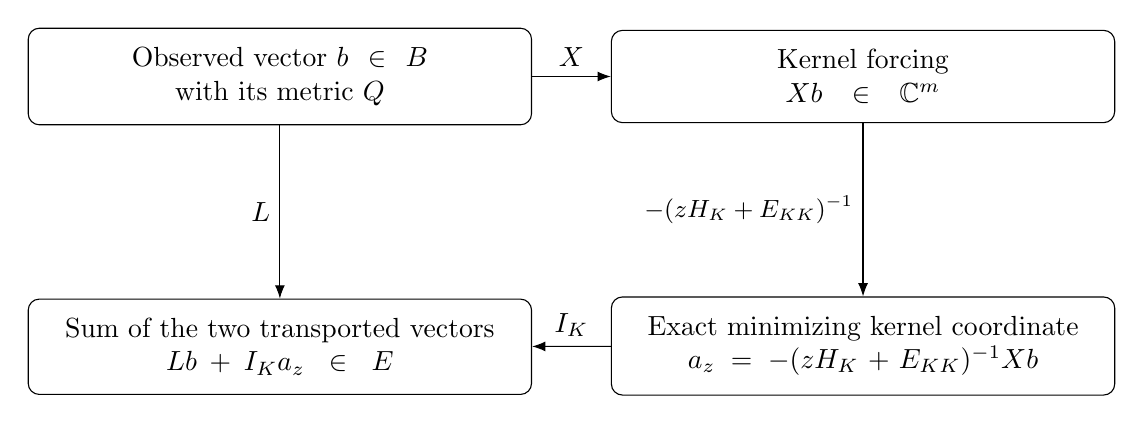
\begin{tikzpicture}[>=Latex,node distance=18mm,
 box/.style={draw,rounded corners,align=center,text width=5.9cm,inner sep=7pt}]
\node[box] (b) {Observed vector $b\in B$\\with its metric $Q$};
\node[box,right=10mm of b] (forcing) {Kernel forcing\\$Xb\in\mathbb C^m$};
\node[box,below=22mm of b] (full) {Sum of the two transported vectors\\$Lb+I_Ka_z\in E$};
\node[box,below=22mm of forcing] (a) {Exact minimizing kernel coordinate\\$a_z=-(zH_K+E_{KK})^{-1}Xb$};
\draw[->] (b)--node[above] {$X$}(forcing);
\draw[->] (b)--node[left] {$L$}(full);
\draw[->] (forcing)--node[left,font=\small] {$-(zH_K+E_{KK})^{-1}$}(a);
\draw[->] (a)--node[above] {$I_K$}(full);
\end{tikzpicture}
\caption{The exact full minimum in RM1--8. The arrows labelled $L$ and
$I_K$ supply the two summands of the full vector. Both cross blocks remain.
The kernel correction is $D(z)=X^*(zH_K+E_{KK})^{-1}X$.
The correction subtracts from $zQ+E_{BB}$, and the observed endomorphism is
$\mathscr Y(z)=z[zQ+E_{BB}-D(z)]^{-1}Q$.
This is the finite Feshbach--Schur construction; the proof cites Dusson,
Sigal and Stamm at its precise original-author source location.}
\end{figure}
The contributing kernel space is the span of $A^jCb$, where
$A=H_K^{-1/2}E_{KK}H_K^{-1/2}$ and $C=H_K^{-1/2}XQ^{-1/2}$.
Its exact dimension is the rank of the phase-bearing moment matrix
$[C^*A^{i+j}C]_{i,j=0}^{m-1}$ (RM12--14). Reducing kernel directions with
zero coupling have an explicitly proved cancellation; none is discarded
on the basis of a rank count alone.
\clearpage
\section*{An exact finite comparison of the three actions}
\addcontentsline{toc}{section}{An exact finite comparison of the three actions}
RM22 evaluates the example $G=I_3$, $T=\operatorname{diag}(0,2,3i)$ and
$\Lambda=\left(\begin{smallmatrix}-1&1&0\\-i&0&1\end{smallmatrix}\right)$.
Its kernel frame is $(1,1,i)^{\mathsf T}$ and
\[
 D(z)=\frac1{9(3z+13)}
 \begin{pmatrix}1&14i\\-14i&196\end{pmatrix}.
\]
\begin{figure}[H]\centering
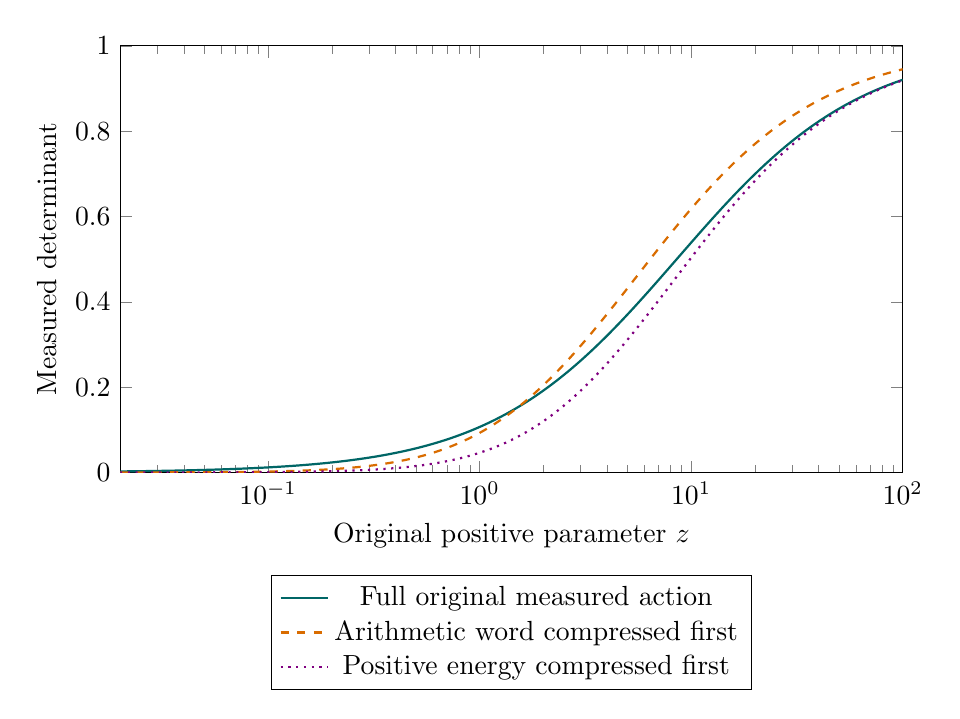
\begin{tikzpicture}\begin{semilogxaxis}[width=.95\textwidth,height=7cm,
 xlabel={Original positive parameter $z$},ylabel={Measured determinant},
 xmin=.02,xmax=100,ymin=0,ymax=1,
 legend style={at={(.5,-.24)},anchor=north,legend columns=1}]
\addplot[teal!80!black,thick]coordinates{(0.0199526231497,0.00239547699581) (0.0210438404302,0.00252612852628) (0.0221947368389,0.00266388533399) (0.0234085762522,0.00280913152506) (0.0246888010491,0.00296227171247) (0.026039041874,0.00312373208213) (0.0274631279327,0.00329396151107) (0.0289650978518,0.00347343273997) (0.0305492111322,0.00366264360232) (0.0322199602284,0.00386211831248) (0.0339820832894,0.00407240881479) (0.0358405775955,0.00429409619643) (0.0378007137302,0.00452779216592) (0.0398680505275,0.0047741406001) (0.0420484508363,0.00503381916161) (0.0443480981473,0.00530754098948) (0.0467735141287,0.00559605646494) (0.0493315771216,0.00590015505502) (0.0520295416463,0.00622066723586) (0.0548750589759,0.00655846649814) (0.0578761988349,0.00691447143644) (0.0610414722843,0.00728964792461) (0.0643798558586,0.00768501137868) (0.0679008170228,0.00810162910896) (0.0716143410213,0.00854062276257) (0.0755309591959,0.00900317085719) (0.0796617788517,0.00949051140702) (0.0840185147571,0.0100039446407) (0.088613522366,0.0105448358116) (0.0934598328571,0.0111146180987) (0.0985711900901,0.0117147955984) (0.103962089582,0.0123469464029) (0.109647819614,0.013012725765) (0.115644504594,0.0137138693435) (0.121969150775,0.0144521965258) (0.128639694494,0.0152296138218) (0.13567505303,0.0160481183218) (0.143095178258,0.0169098012113) (0.15092111323,0.0178168513313) (0.159175051849,0.0187715587751) (0.167880401812,0.0197763185069) (0.177061850996,0.0208336339874) (0.186745437464,0.0219461207904) (0.196958623314,0.0231165101907) (0.207730372557,0.0243476527002) (0.219091233259,0.0256425215302) (0.23107342417,0.0270042159501) (0.243710926098,0.028435964514) (0.257039578277,0.0299411281203) (0.271097180002,0.0315232028677) (0.285923597827,0.0331858226669) (0.301560878626,0.0349327615628) (0.318053368833,0.0367679357186) (0.335447840207,0.0386954050092) (0.353793622474,0.0407193741666) (0.373142743223,0.0428441934148) (0.393550075456,0.0450743585289) (0.415073493198,0.0474145102477) (0.437774035632,0.0498694329637) (0.461716080198,0.0524440526119) (0.486967525166,0.055143433673) (0.513599982189,0.0579727752038) (0.541688979393,0.0609374058032) (0.571314175567,0.0640427774194) (0.602559586074,0.067294457902) (0.635513821112,0.0706981221998) (0.670270337006,0.0742595421051) (0.706927701248,0.077984574445) (0.745589872028,0.0818791476225) (0.78636649305,0.0859492464116) (0.82937320448,0.0902008949157) (0.874731970892,0.0946401376051) (0.922571427155,0.0992730183575) (0.97302724323,0.104105557434) (1.02624250893,0.10914372634) (1.0823681397,0.11439342053) (1.14156330462,0.119860429937) (1.2039958778,0.125550407327) (1.26984291443,0.131468834507) (1.33929115297,0.137620986431) (1.41253754462,0.144011893286) (1.48978981198,0.150646300677) (1.57126703806,0.157528628058) (1.65720028761,0.164662925587) (1.74783326242,0.172052829648) (1.84342299241,0.179701517298) (1.9442405646,0.187611659961) (2.05057189185,0.195785376719) (2.16271852373,0.204224187609) (2.28099850167,0.212928967376) (2.40574726093,0.221899900155) (2.53731858186,0.231136435635) (2.6760855932,0.240637247239) (2.82244183025,0.25040019293) (2.97680235095,0.260422279257) (3.13960491288,0.270699629255) (3.31131121483,0.28122745485) (3.49240820602,0.292000034377) (3.68340946719,0.303010695843) (3.88485666698,0.314251806494) (4.09732109814,0.325714769232) (4.32140529763,0.337390026351) (4.55774475544,0.349267071008) (4.80700971675,0.361334466736) (5.06990708275,0.373579875227) (5.34718241532,0.385990092491) (5.63962205146,0.398551093389) (5.94805533325,0.411248084396) (6.27335695984,0.424065564325) (6.61644946805,0.436987392617) (6.9783058486,0.449996864652) (7.3599523055,0.463076793414) (7.76247116629,0.476209596738) (8.18700395142,0.489377389226) (8.63475461161,0.502562077856) (9.10699294213,0.515745460215) (9.60505818387,0.528909324226) (10.1303628214,0.542035548235) (10.6843965886,0.555106200251) (11.2687306935,0.568103635227) (11.8850222744,0.581010589222) (12.5350190988,0.593810269405) (13.2205645205,0.606486438901) (13.9436027073,0.619023495598) (14.706184154,0.631406544137) (15.5104714981,0.643621460424) (16.3587456524,0.65565494816) (17.2534122739,0.667494586998) (18.1970085861,0.67912887209) (19.1922105741,0.690547244934) (20.2418405738,0.701740115541) (21.3488752759,0.712698876093) (22.5164541674,0.723415906361) (23.7478884355,0.733884571268) (25.0466703572,0.74409921106) (26.4164832039,0.754055124633) (27.8612116863,0.763748546613) (29.3849529719,0.773176618837) (30.9920283039,0.782337356903) (32.6869952559,0.791229612492) (34.4746606573,0.799853032126) (36.360094225,0.808208013069) (38.3486429408,0.816295657) (40.4459462152,0.824117722105) (42.6579518802,0.83167657417) (44.9909330574,0.838975137218) (47.4515059481,0.84601684419) (50.0466485963,0.852805588128) (52.7837206782,0.859345674241) (55.6704843735,0.865641773216) (58.7151263793,0.871698876062) (61.9262811259,0.877522250724) (65.3130552647,0.88311740069) (68.8850534936,0.888490025716) (72.6524057951,0.893645984806) (76.625796165,0.898591261513) (80.8164929113,0.903331931606) (85.2363806101,0.907874133115) (89.8979938103,0.912224038743) (94.8145525805,0.916387830607) (100,0.920371677252)};\addlegendentry{Full original measured action}
\addplot[orange!85!black,thick,dashed]coordinates{(0.0199526231497,9.67293806473e-05) (0.0210438404302,0.000107433297735) (0.0221947368389,0.000119311865618) (0.0234085762522,0.000132492328363) (0.0246888010491,0.000147115434246) (0.026039041874,0.000163336822253) (0.0274631279327,0.000181328543211) (0.0289650978518,0.000201280727309) (0.0305492111322,0.000223403410653) (0.0322199602284,0.000247928534283) (0.0339820832894,0.000275112129974) (0.0358405775955,0.000305236707989) (0.0378007137302,0.000338613862801) (0.0398680505275,0.000375587113648) (0.0420484508363,0.00041653499758) (0.0443480981473,0.000461874433421) (0.0467735141287,0.000512064375727) (0.0493315771216,0.000567609778423) (0.0520295416463,0.00062906588826) (0.0548750589759,0.000697042888507) (0.0578761988349,0.000772210913442) (0.0610414722843,0.000855305454048) (0.0643798558586,0.000947133174937) (0.0679008170228,0.00104857816179) (0.0716143410213,0.00116060861749) (0.0755309591959,0.00128428402362) (0.0796617788517,0.00142076278188) (0.0840185147571,0.00157131034747) (0.088613522366,0.00173730786315) (0.0934598328571,0.00192026129895) (0.0985711900901,0.00212181109758) (0.103962089582,0.00234374232026) (0.109647819614,0.00258799528128) (0.115644504594,0.00285667665222) (0.121969150775,0.00315207100836) (0.128639694494,0.00347665278083) (0.13567505303,0.00383309856708) (0.143095178258,0.00422429974147) (0.15092111323,0.00465337529491) (0.159175051849,0.00512368481926) (0.167880401812,0.00563884153789) (0.177061850996,0.0062027252688) (0.186745437464,0.00681949519092) (0.196958623314,0.00749360226811) (0.207730372557,0.00822980116915) (0.219091233259,0.0090331615055) (0.23107342417,0.00990907819296) (0.243710926098,0.0108632807279) (0.257039578277,0.0119018411546) (0.271097180002,0.0130311804879) (0.285923597827,0.0142580733437) (0.301560878626,0.0155896505232) (0.318053368833,0.0170333992884) (0.335447840207,0.0185971610668) (0.353793622474,0.0202891263224) (0.373142743223,0.0221178263361) (0.393550075456,0.0240921216468) (0.415073493198,0.0262211869206) (0.437774035632,0.0285144920309) (0.461716080198,0.0309817791582) (0.486967525166,0.0336330357441) (0.513599982189,0.0364784631685) (0.541688979393,0.0395284410547) (0.571314175567,0.0427934871475) (0.602559586074,0.0462842127581) (0.635513821112,0.0500112738127) (0.670270337006,0.0539853175971) (0.706927701248,0.0582169253422) (0.745589872028,0.0627165508488) (0.78636649305,0.0674944554112) (0.82937320448,0.0725606393524) (0.874731970892,0.077924770545) (0.922571427155,0.0835961103475) (0.97302724323,0.0895834374433) (1.02624250893,0.095894970126) (1.0823681397,0.102538287627) (1.14156330462,0.109520251131) (1.2039958778,0.116846925183) (1.26984291443,0.124523500213) (1.33929115297,0.132554216976) (1.41253754462,0.140942293699) (1.48978981198,0.149689856807) (1.57126703806,0.158797876051) (1.65720028761,0.16826610495) (1.74783326242,0.178093027387) (1.84342299241,0.188275811242) (1.9442405646,0.198810269893) (2.05057189185,0.20969083238) (2.16271852373,0.220910522983) (2.28099850167,0.232460950897) (2.40574726093,0.244332310579) (2.53731858186,0.256513393263) (2.6760855932,0.268991610011) (2.82244183025,0.281753026532) (2.97680235095,0.294782409846) (3.13960491288,0.308063286732) (3.31131121483,0.321578013696) (3.49240820602,0.335307858058) (3.68340946719,0.349233089554) (3.88485666698,0.363333081674) (4.09732109814,0.377586421828) (4.32140529763,0.391971029218) (4.55774475544,0.406464279205) (4.80700971675,0.421043132813) (5.06990708275,0.435684269925) (5.34718241532,0.450364224659) (5.63962205146,0.465059521349) (5.94805533325,0.479746809592) (6.27335695984,0.494402996786) (6.61644946805,0.509005376674) (6.9783058486,0.523531752481) (7.3599523055,0.537960553317) (7.76247116629,0.552270942687) (8.18700395142,0.566442918054) (8.63475461161,0.580457400607) (9.10699294213,0.594296314541) (9.60505818387,0.607942655336) (10.1303628214,0.621380546731) (10.6843965886,0.634595286245) (11.2687306935,0.647573379283) (11.8850222744,0.660302562043) (12.5350190988,0.672771813557) (13.2205645205,0.684971357381) (13.9436027073,0.696892653514) (14.706184154,0.70852838126) (15.5104714981,0.719872413819) (16.3587456524,0.730919785417) (17.2534122739,0.741666651874) (18.1970085861,0.752110245481) (19.1922105741,0.762248825085) (20.2418405738,0.772081622257) (21.3488752759,0.781608784401) (22.5164541674,0.790831315596) (23.7478884355,0.799751015962) (25.0466703572,0.808370420237) (26.4164832039,0.816692736217) (27.8612116863,0.824721783651) (29.3849529719,0.832461934102) (30.9920283039,0.839918052221) (32.6869952559,0.847095438837) (34.4746606573,0.853999776162) (36.360094225,0.860637075402) (38.3486429408,0.867013626952) (40.4459462152,0.873135953356) (42.6579518802,0.879010765116) (44.9909330574,0.884644919428) (47.4515059481,0.890045381864) (50.0466485963,0.895219190987) (52.7837206782,0.900173425872) (55.6704843735,0.904915176457) (58.7151263793,0.90945151665) (61.9262811259,0.913789480083) (65.3130552647,0.917936038411) (68.8850534936,0.921898082018) (72.6524057951,0.925682403013) (76.625796165,0.929295680371) (80.8164929113,0.93274446708) (85.2363806101,0.936035179166) (89.8979938103,0.939174086451) (94.8145525805,0.942167304901) (100,0.945020790457)};\addlegendentry{Arithmetic word compressed first}
\addplot[violet,thick,dotted]coordinates{(0.0199526231497,3.27032512943e-05) (0.0210438404302,3.63498039458e-05) (0.0221947368389,4.04012568731e-05) (0.0234085762522,4.49022765236e-05) (0.0246888010491,4.99024067841e-05) (0.026039041874,5.54565930799e-05) (0.0274631279327,6.16257613447e-05) (0.0289650978518,6.84774573639e-05) (0.0305492111322,7.60865525003e-05) (0.0322199602284,8.4536022362e-05) (0.0339820832894,9.39178055648e-05) (0.0358405775955,0.000104333750376) (0.0378007137302,0.000115896657709) (0.0398680505275,0.000128731429665) (0.0420484508363,0.000142976333586) (0.0443480981473,0.00015878439242) (0.0467735141287,0.000176324913058) (0.0493315771216,0.000195785165209) (0.0520295416463,0.000217372224361) (0.0548750589759,0.000241314993353) (0.0578761988349,0.000267866418138) (0.0610414722843,0.000297305914352) (0.0643798558586,0.000329942022441) (0.0679008170228,0.000366115310123) (0.0716143410213,0.000406201542149) (0.0755309591959,0.000450615138309) (0.0796617788517,0.000499812941757) (0.0840185147571,0.000554298320657) (0.088613522366,0.000614625627068) (0.0934598328571,0.000681405037788) (0.0985711900901,0.000755307802467) (0.103962089582,0.000837071924771) (0.109647819614,0.000927508302553) (0.115644504594,0.00102750735289) (0.121969150775,0.00113804614739) (0.128639694494,0.0012601960823) (0.13567505303,0.00139513110659) (0.143095178258,0.00154413652914) (0.15092111323,0.00170861842377) (0.159175051849,0.0018901136472) (0.167880401812,0.00209030048112) (0.177061850996,0.00231100990405) (0.186745437464,0.00255423749286) (0.196958623314,0.00282215594597) (0.207730372557,0.00311712821213) (0.219091233259,0.00344172119813) (0.23107342417,0.00379872001785) (0.243710926098,0.00419114273181) (0.257039578277,0.00462225551191) (0.271097180002,0.00509558814997) (0.285923597827,0.00561494981095) (0.301560878626,0.00618444491227) (0.318053368833,0.00680848899015) (0.335447840207,0.00749182439134) (0.353793622474,0.00823953560571) (0.373142743223,0.00905706403042) (0.393550075456,0.00995022193198) (0.415073493198,0.0109252053471) (0.437774035632,0.0119886056383) (0.461716080198,0.0131474193971) (0.486967525166,0.0144090563624) (0.513599982189,0.0157813450063) (0.541688979393,0.0172725354146) (0.571314175567,0.0188912990824) (0.602559586074,0.0206467252321) (0.635513821112,0.0225483132564) (0.670270337006,0.0246059608946) (0.706927701248,0.026829947756) (0.745589872028,0.0292309138258) (0.78636649305,0.0318198326103) (0.82937320448,0.0346079786174) (0.874731970892,0.0376068889112) (0.922571427155,0.0408283185341) (0.97302724323,0.0442841896565) (1.02624250893,0.0479865343848) (1.0823681397,0.0519474312471) (1.14156330462,0.0561789354632) (1.2039958778,0.0606930032079) (1.26984291443,0.0655014101833) (1.33929115297,0.0706156649233) (1.41253754462,0.0760469173701) (1.48978981198,0.0818058633762) (1.57126703806,0.087902645898) (1.65720028761,0.0943467537572) (1.74783326242,0.101146918951) (1.84342299241,0.108311013587) (1.9442405646,0.115845947601) (2.05057189185,0.123757568489) (2.16271852373,0.132050564345) (2.28099850167,0.14072837152) (2.40574726093,0.149793088247) (2.53731858186,0.159245395574) (2.6760855932,0.169084486908) (2.82244183025,0.179308007433) (2.97680235095,0.189912004587) (3.13960491288,0.200890890681) (3.31131121483,0.212237418618) (3.49240820602,0.223942671529) (3.68340946719,0.235996066959) (3.88485666698,0.248385376076) (4.09732109814,0.261096758139) (4.32140529763,0.274114810255) (4.55774475544,0.287422632248) (4.80700971675,0.301001906196) (5.06990708275,0.314832989987) (5.34718241532,0.328895024015) (5.63962205146,0.343166049904) (5.94805533325,0.357623139978) (6.27335695984,0.372242535995) (6.61644946805,0.386999795513) (6.9783058486,0.401869944137) (7.3599523055,0.416827631815) (7.76247116629,0.431847291268) (8.18700395142,0.446903296652) (8.63475461161,0.46197012055) (9.10699294213,0.477022487451) (9.60505818387,0.492035521966) (10.1303628214,0.506984890149) (10.6843965886,0.521846932447) (11.2687306935,0.536598786969) (11.8850222744,0.551218501965) (12.5350190988,0.565685136615) (13.2205645205,0.579978849431) (13.9436027073,0.594080973806) (14.706184154,0.607974080463) (15.5104714981,0.621642026742) (16.3587456524,0.635069992896) (17.2534122739,0.648244505716) (18.1970085861,0.66115344998) (19.1922105741,0.673786068377) (20.2418405738,0.686132950641) (21.3488752759,0.698186012775) (22.5164541674,0.709938467263) (23.7478884355,0.721384785269) (25.0466703572,0.732520651818) (26.4164832039,0.743342914969) (27.8612116863,0.753849529998) (29.3849529719,0.764039499551) (30.9920283039,0.773912810724) (32.6869952559,0.783470369941) (34.4746606573,0.792713936479) (36.360094225,0.801646055381) (38.3486429408,0.81026999046) (40.4459462152,0.818589658014) (42.6579518802,0.826609561784) (44.9909330574,0.834334729629) (47.4515059481,0.841770652321) (50.0466485963,0.848923224776) (52.7837206782,0.855798689991) (55.6704843735,0.862403585884) (58.7151263793,0.868744695191) (61.9262811259,0.874828998502) (65.3130552647,0.880663630502) (68.8850534936,0.886255839413) (72.6524057951,0.89161294962) (76.625796165,0.896742327427) (80.8164929113,0.901651349856) (85.2363806101,0.906347376403) (89.8979938103,0.91083772362) (94.8145525805,0.9151296424) (100,0.919230297831)};\addlegendentry{Positive energy compressed first}
\end{semilogxaxis}\end{tikzpicture}
\caption{Exact rational functions from RM22, sampled only to draw the curves.
The full action is always above the compressed positive-energy action (RM15).
Its comparison with the compressed arithmetic word changes sign at
$z=(\sqrt{11335}-47)/39$. The figure is an auxiliary finite example,
not a native period calculation. All source coordinates and phases are
specified in RM22 and the reproducible builder.}
\end{figure}
For the actual growing-dimensional word, a coherent full metric enclosure
$\alpha G\preceq\widetilde G\preceq\beta G$ gives the uniform bound
\[
 |\log\det\mathscr Y_{\widetilde G}(z)-\log\det\mathscr Y_G(z)|
 \le (\Delta+p)\log(\beta/\alpha),
\]
where $\Delta=\operatorname{rank}T$ and $p=\operatorname{rank}(TI_K)$.
RM19--21 proves the moving-section comparison. Fixed enclosure ratios cost
$O(k)$ on the original word, below its $kq$ determinant scale.
\clearpage
\section*{Every original lower-root constraint in the sampling map}
\addcontentsline{toc}{section}{Every original lower-root constraint in the sampling map}
The row functions give physical moments
$L_N[j,n]=(-i)^nn![w^n]A_{z_j}(w)$. The matrix $J_N$ contains all coefficient
columns of multiplication by the full monic lower polynomial $Q_-$.
The exact relation to the orthogonal projection is
\[
 \begin{array}{ccc}
 \mathcal P_{N-v-q'}&\xrightarrow{\ J_N:\ p\mapsto Q_-p\ }&\mathcal P_{N-v}\\
 &&\downarrow L_N\\
 &&\mathbb C^r.
 \end{array}
\]
\[
 C_N=(L_NJ_N)(J_N^*H_NJ_N)^{-1}(L_NJ_N)^*,\qquad
 B_N=L_NH_N^{-1}L_N^*.
\]
Here $H_N$ is the full physical Gamma Gram; its mass remains $\sqrt{2\pi}$.
CS19 proves this map equals the full lower-root projector. CS21--23 keeps
the error in every coefficient of $J_N$, through the original metric,
before any determinant is taken. The result is a certified approximation
of these complete maps. The sample count alone is not a count of bit
operations, zero isolation or numerical evaluation of the native period.
\clearpage

\clearpage\part{The complete measured resolvent and kernel memory}
\section{The exact kernel memory of the original measured resolvent}\label{the-exact-kernel-memory-of-the-original-measured-resolvent}

22 September 2026. Result SZ-20260922-020, root derivation RM1--RM23.

The received PR1--PR44 calculation evaluates a determinant of the full observed resolvent. This continuation identifies the entire matrix correction produced by the observation kernel, constructs the smallest kernel space that carries that correction, and proves its exact reconstruction from the observed family. Every original metric, observation, word and complex cross term remains in the formulas. The construction applies directly to the programme's word \(T_k=D_k(M)\) and its canonical metrics at the four original cutoffs. It does not assign the unresolved native determinant coefficient.

The elimination used here is the finite positive-metric Feshbach--Schur map. Its human source is Geneviève Dusson, Israel Michael Sigal and Benjamin Stamm, \href{https://arxiv.org/abs/2105.02058v1}{\emph{The Feshbach--Schur map and perturbation theory}}, original author TeX \texttt{AriFestFSM\_arxiv.tex}, theorem \texttt{thm:isospF}, equations \texttt{Fesh}, \texttt{QP}, \texttt{Hlam-deco}, \texttt{Ulam-def}, source lines 398--489. The exact substitution is their operator \(H-\lambda\) with our \(T^{\dagger_G}T+zI\), their projection with the original minimum-section projection \(L\Lambda\), and \(\lambda=-z\). The finite proofs below also supply the complete elimination and reconstruction explicitly. This is a use of that established construction, not a claim of inventing it.

\subsection{RM1. Original value and kernel coordinates}\label{rm1.-original-value-and-kernel-coordinates}

Let \(E=\mathbb C^q\) carry the positive Hermitian metric \(G\), let \(\Lambda:E\to B=\mathbb C^n\) be onto, and let \(K=\ker\Lambda\), \(m=q-n\). Let \(I_K:\mathbb C^m\to E\) be a fixed full frame of the actual kernel, and retain a linear word \(T:E\to E\). Put

\[
 Q=(\Lambda G^{-1}\Lambda^*)^{-1},\quad
 L=G^{-1}\Lambda^*Q,\quad H_K=I_K^*GI_K,\quad H=T^{\dagger_G}T=G^{-1}T^*GT.
 \tag{RM1}
\]

Then \(\Lambda L=I_n\), \(L^*GL=Q\), and \(I_K^*GL=0\). In particular the map

\[
 U_0:B\oplus\mathbb C^m\longrightarrow E,\qquad U_0(b,a)=Lb+I_Ka
 \tag{RM2}
\]

is an isomorphism with source metric \(\operatorname{diag}(Q,H_K)\). Indeed applying \(\Lambda\) to a zero image gives \(b=0\), then injectivity of \(I_K\) gives \(a=0\); dimensions finish the proof. The orthogonality follows by direct substitution in RM1. This proves the coordinate map without replacing the value metric or kernel metric by a different source.

Define the three energy blocks

\[
 E_{BB}=L^*T^*GTL,\qquad X=I_K^*T^*GTL,\qquad E_{KK}=I_K^*T^*GTI_K.
 \tag{RM3}
\]

Thus \(U_0^*T^*GTU_0=\begin{psmallmatrix}E_{BB}&X^*\\X&E_{KK}\end{psmallmatrix}\succeq0\). Notice that \(E_{KK}\) is the energy of the full rectangular map \(T I_K\). No compressed arithmetic endomorphism has been substituted.

\subsection{RM2. The complete attained minimum at every positive parameter}\label{rm2.-the-complete-attained-minimum-at-every-positive-parameter}

For \(z>0\), set

\[
 D(z)=X^*(zH_K+E_{KK})^{-1}X,\quad
 F(z)=zQ+E_{BB}-D(z).
 \tag{RM4}
\]

The matrix \(F(z)\) is positive definite. More precisely, for every \(b\in B\),

\[
 b^*F(z)b=z\,b^*Qb+
 \min_{a\in\mathbb C^m}\left\{\|T(Lb+I_Ka)\|_G^2+z\,a^*H_Ka\right\}.
 \tag{RM5}
\]

The unique minimizer is

\[
 a_z(b)=-(zH_K+E_{KK})^{-1}Xb.
 \tag{RM6}
\]

To prove both statements, expand the braces using RM3, then complete the square with its strictly positive \(a\)-block. The remaining quadratic form is \(E_{BB}-D(z)\succeq0\). Adding \(zQ>0\) proves strict positivity. This also specifies the map lifting each observed vector back to its exact minimizing full vector \(Lb+I_Ka_z(b)\).

\subsection{RM3. Matrix recovery of the full measured resolvent}\label{rm3.-matrix-recovery-of-the-full-measured-resolvent}

Retain the actual observed family

\[
 \mathscr Y(z)=\Lambda z(zI+H)^{-1}L.
\]

Solving the two block equations of \(U_0^*G(zI+H)U_0\), whose right-hand side for an observed input \(b\) is \(z(Qb,0)^T\), gives

\[
 \boxed{\mathscr Y(z)=zF(z)^{-1}Q.}
 \tag{RM7}
\]

Consequently the entire memory matrix is recoverable from the original observed family:

\[
 \boxed{D(z)=E_{BB}-zQ\bigl(\mathscr Y(z)^{-1}-I\bigr).}
 \tag{RM8}
\]

The multiplication order in RM7--RM8 is essential. For example \(\mathscr Y(z)\) need not be Hermitian in the original coefficient frame; \(Q\mathscr Y(z)\) is Hermitian. The high-parameter coefficient also recovers \(E_{BB}\):

\[
 E_{BB}=\lim_{z\to\infty}zQ\bigl(\mathscr Y(z)^{-1}-I\bigr),
 \tag{RM9}
\]

because \(D(z)=O(z^{-1})\). All these statements are finite exact identities in the displayed maps.

\subsection{RM4. The positive memory measure and its complete kernel space}\label{rm4.-the-positive-memory-measure-and-its-complete-kernel-space}

For the sole purpose of expressing the same metric in an orthonormal frame, define

\[
 A=H_K^{-1/2}E_{KK}H_K^{-1/2},\quad
 C=H_K^{-1/2}XQ^{-1/2},\quad B=Q^{-1/2}E_{BB}Q^{-1/2}.
 \tag{RM10}
\]

The inverse coordinate maps are specified by \(I_KH_K^{-1/2}\) and \(LQ^{-1/2}\); thus no original mass or norm is removed. Write \(A=\sum_{\lambda\ge0}\lambda P_\lambda\), with its complete spectral projections, including multiplicities. Positivity of RM3 implies \(P_0C=0\). One proof is that a vector \(a\in\ker A\) gives zero energy to \(TI_KH_K^{-1/2}a\), hence this vector is zero and its energy pairing with \(TLQ^{-1/2}b\) vanishes for every \(b\).

Therefore

\[
 \widehat D(z):=Q^{-1/2}D(z)Q^{-1/2}
 =\sum_{\lambda>0}\frac{M_\lambda}{z+\lambda},\qquad
 M_\lambda=C^*P_\lambda C\succeq0.
 \tag{RM11}
\]

This is a finite matrix Stieltjes transform: the definition here is exactly a sum of positive matrix masses divided by \(z+\lambda\) for positive real \(\lambda\). Repeated kernel energies use one full residue \(M_\lambda\); no arbitrary eigenvector choice enters it. At a zero energy, the residue vanishes by the proved relation \(P_0C=0\), rather than by deletion.

Define the actual observable kernel subspace

\[
 \mathcal H_{\rm mem}=\operatorname{span}\{A^jCb:b\in\mathbb C^n,\ 0\le j<m\}\subseteq\mathbb C^m.
 \tag{RM12}
\]

Cayley--Hamilton shows that this space is \(A\)-invariant. Since \(A=A^*\), its orthogonal complement is invariant too. Spectral interpolation by polynomials in \(A\) then proves

\[
 \mathcal H_{\rm mem}=\bigoplus_{\lambda>0}\operatorname{ran}(P_\lambda C),\qquad
 \dim\mathcal H_{\rm mem}=\sum_{\lambda>0}\operatorname{rank}M_\lambda.
 \tag{RM13}
\]

For the rank statement use \(M_\lambda=(P_\lambda C)^*(P_\lambda C)\), so both matrices have the same null space. The inclusion \(I_KH_K^{-1/2}:\mathcal H_{\rm mem}\hookrightarrow K\subset E\) is the exact connecting isometry to the programme. The orthogonal complement is retained as a reducing kernel space with zero coupling to the observation.

\subsection{RM5. Minimality and uniqueness, with a finite moment certificate}\label{rm5.-minimality-and-uniqueness-with-a-finite-moment-certificate}

Any representation of RM11 in the form \(C_1^*(zI+A_1)^{-1}C_1\), with \(A_1\succeq0\) and no zero residue, has a residue \(C_1^*P_{1,\lambda}C_1=M_\lambda\) at each actual pole. The dimension of its \(\lambda\)-eigenspace is at least \(\operatorname{rank}M_\lambda\). Summing gives the lower bound in RM13. Restriction to \(\mathcal H_{\rm mem}\) attains it, so this is a smallest realization of the original memory.

It is unique up to an isometry that also intertwines \(A\) and \(C\). Here is a direct proof. Equality of the rational functions gives equality of their expansions at infinity, hence

\[
 C^*A^jC=C_1^*A_1^jC_1\quad(j\ge0).
\]

Send each vector \(\sum_j A^jCb_j\) to \(\sum_j A_1^jC_1b_j\). The squared norm and every cross inner product are the same, by the moment identities with exponent \(i+j\). The map is well-defined, isometric, onto the generated spaces, and intertwines \(A\) and \(A_1\). It also maps \(C\) to \(C_1\). This proves the assertion.

There is an exact finite rank certificate. The block matrix

\[
 \mathcal M_m=[C^*A^{i+j}C]_{i,j=0}^{m-1}
\]

is the Gram matrix of \([C,AC,\ldots,A^{m-1}C]\). Thus

\[
 \boxed{\operatorname{rank}\mathcal M_m=\dim\mathcal H_{\rm mem}.}
 \tag{RM14}
\]

It uses the original phase-bearing moments, not their scalar traces.

\subsection{RM6. The exact correction to compressing before taking the resolvent}\label{rm6.-the-exact-correction-to-compressing-before-taking-the-resolvent}

In the orthonormal value frame the compression of the positive energy \(H\) is \(B\). Put

\[
 F_0=zI+B,\qquad R(z)=F_0^{-1/2}\widehat D(z)F_0^{-1/2}.
\]

RM5 gives \(0\preceq R(z)\prec I\). Comparing the correct family with \(Y_{\rm energy}(z)=z(zI+B)^{-1}\) gives

\[
 \widehat{\mathscr Y}(z)\succeq Y_{\rm energy}(z),\qquad
 \log\frac{\det\mathscr Y(z)}{\det Y_{\rm energy}(z)}
 =-\log\det(I-R(z))\ge0.
 \tag{RM15}
\]

Both statements follow by inversion and the factorization of \(F_0-\widehat D\). The rank of \(R(z)\) equals \(\operatorname{rank}C\), and the exact correction is the sum \(-\sum_{j=1}^{\operatorname{rank}C}\log(1-r_j(z))\). In particular it vanishes at one positive \(z\) if and only if \(C=0\), which is equivalent to \(K\) reducing the positive energy \(H\). This proves precisely when the omission is allowed.

For comparison with the arithmetic operator compressed first, write the full word itself in the same orthogonal splitting:

\[
 \widetilde T=\begin{pmatrix}T_{BB}&T_{BK}\\T_{KB}&T_{KK}\end{pmatrix}.
\]

Then

\[
 B=T_{BB}^*T_{BB}+T_{KB}^*T_{KB},\quad
 C=T_{BK}^*T_{BB}+T_{KK}^*T_{KB},\quad
 A=T_{BK}^*T_{BK}+T_{KK}^*T_{KK}.
 \tag{RM16}
\]

Substitution in RM7 proves the complete relation to the resolvent of \(T_{BB}^*T_{BB}\): its missing effective term is \(T_{KB}^*T_{KB}-C^*(zI+A)^{-1}C\). Its sign is not fixed. Indeed with scalar blocks, \(T=\begin{psmallmatrix}0&0\\1&0\end{psmallmatrix}\) gives positive term \(1\), while \(T=\begin{psmallmatrix}1&1\\0&0\end{psmallmatrix}\) gives negative term \(-1/(z+1)\). These exact words have positive full energies. Thus the defect defines the specified memory family; it is not a reason to end the calculation.

\subsection{RM7. Every zero direction and every determinant factor}\label{rm7.-every-zero-direction-and-every-determinant-factor}

The full energy in this frame is \(\begin{psmallmatrix}B&C^*\\C&A\end{psmallmatrix}\). Let \(\mathcal H_{\rm inv}=\mathcal H_{\rm mem}^{\perp}\subset K\). It is reducing and has no coupling to \(B\). Hence

\[
 \det(zI+H)=\det(zI+A|_{\mathcal H_{\rm inv}})
 \det\begin{pmatrix}zI+B&C_{\rm mem}^*\\C_{\rm mem}&zI+A_{\rm mem}\end{pmatrix}.
\]

The same factor occurs in \(\det(zI+A)\) in the numerator of PR7 and cancels exactly. It includes every zero direction of \(K\cap\ker T\), since those are in \(\mathcal H_{\rm inv}\). The invariant space and its energy are retained explicitly; they have zero residue in RM11. The cancellation therefore has a proved map and a precise mathematical reason.

The remaining determinant identity is

\[
 \det\mathscr Y(z)=
 z^n\frac{\det(zI+A_{\rm mem})}
 {\det\begin{pmatrix}zI+B&C_{\rm mem}^*\\C_{\rm mem}&zI+A_{\rm mem}\end{pmatrix}}.
 \tag{RM17}
\]

It is the PR determinant formula with all unobserved reducing factors canceled by exact equality, not by an asymptotic allocation.

\subsection{RM8. Application to the original mixed arithmetic family}\label{rm8.-application-to-the-original-mixed-arithmetic-family}

For each original \(N\in\{q-1,q,2q-1,2q\}\), use \(T=T_k=D_k(M)\), the unchanged \(G_N,\Lambda,I_K\), and \(m=8k-16\). Then RM4 is the explicit original-metric matrix

\[
 D_N(z)=L_N^*T_k^*G_NT_kI_K
 (zH_{K,N}+H_{TK,N})^{-1}
 I_K^*T_k^*G_NT_kL_N.
 \tag{RM18}
\]

The received PR19 gives \(H_{TK,N}=J^*\mathfrak G_NJ\) with the fixed exact map \(J=V_O^{-1}\pi_\partial I_K\); this is also the image map proved in the full-word calculation. Substituting that image Gram in RM18 leaves the complete original \(H_{K,N}\) and both complex cross blocks. The positive word spectrum alone does not determine RM18, whereas the full measured family determines it by RM8--RM9.

The finite sign and deep-regularizer results PR25--PR31 are preserved at their stated analytic input status. RM18 neither replaces their native kernel coefficient nor derives a sign of a different complex current. It supplies the exact matrix object that carries the mixed kernel/observation coupling, and RM12--RM14 give a concrete finite construction and rank test for all of its contributing directions. These are the next matrices to evaluate with the complete-row sampling bounds; a determinant bound on them does not erase the off-diagonal terms.

\subsection{RM9. Coherent error in the original full source metric}\label{rm9.-coherent-error-in-the-original-full-source-metric}

Keep exactly the same linear maps \(T,\Lambda,I_K\). Let \(G\) and \(\widetilde G\) be two positive Hermitian forms on that same original space, and let positive numbers \(\alpha\le\beta\) satisfy \[
 \alpha G\preceq\widetilde G\preceq\beta G,\qquad \kappa=\beta/\alpha.
\] Every object bearing a tilde is recomputed from that full form by RM1--7; in particular its minimum section is recomputed, rather than held fixed when its defining metric changes. Write \(\Delta=\operatorname{rank}T\), \(p=\operatorname{rank}(T I_K)\), and let \(\lambda_1,\ldots,\lambda_\Delta>0\) be the positive eigenvalues of \(G^{-1}T^*GT\), in decreasing order. Let \(a_1,\ldots,a_p>0\) be the positive generalized eigenvalues of \((I_K^*T^*GTI_K,I_K^*GI_K)\). The remaining eigenvalues in both lists are exactly zero and their multiplicities depend only on the fixed maps.

For every vector \(x\ne0\), the two Rayleigh quotients of the full positive energy satisfy \[
 \kappa^{-1}\frac{\|Tx\|_G^2}{\|x\|_G^2}
 \le\frac{\|Tx\|_{\widetilde G}^2}{\|x\|_{\widetilde G}^2}
 \le\kappa\frac{\|Tx\|_G^2}{\|x\|_G^2}.
\] The identical proof for \(x=I_Kb\) applies on the complete kernel. The min--max formula now gives, in the same ordering, \[
 \kappa^{-1}\lambda_j\le\widetilde\lambda_j\le\kappa\lambda_j,
 \qquad \kappa^{-1}a_j\le\widetilde a_j\le\kappa a_j.
 \tag{RM19}
\] For clarity, this use of min--max is finite: choose an orthonormal eigenbasis for either Hermitian representative, express a vector's quotient as its eigenvalue-weighted squared coordinates, and maximize the minimum over subspaces of prescribed dimension. Intersection with the span of the smaller eigenvectors proves the upper bound, while the span of the larger eigenvectors attains equality. This argument permits repeated eigenvalues. Applying the pointwise quotient comparison on every such subspace proves RM19.

The original block determinant in RM7, before any reducing-factor cancellation, is \[
 \det\mathscr Y_G(z)=z^{\Delta-p}
 \frac{\prod_{j=1}^{p}(z+a_j)}{\prod_{j=1}^{\Delta}(z+\lambda_j)}.
\] Indeed its numerator is \(z^n\det(zI_m+A)\), its denominator is \(\det(zI_q+H)\), and \(n=q-m\); the zero multiplicities therefore give \(z^{n+m-p-(q-\Delta)}=z^{\Delta-p}\). The identical power occurs for \(\widetilde G\). By RM19, each remaining positive factor changes by a ratio in \([\kappa^{-1},\kappa]\) for every \(z>0\). Thus \[
 \boxed{\left|\log\det\mathscr Y_{\widetilde G}(z)
       -\log\det\mathscr Y_G(z)\right|
 \le(\Delta+p)\log\kappa.}
 \tag{RM20}
\] This bound is uniform in the regularizer, including values smaller than every positive energy. It counts the actual nonzero energies and keeps all exact zero factors before canceling them. It also includes the metric-induced change of the original section, since both determinants were derived with their own RM1 section.

For the programme word, \(\Delta=16k-48\), \(p=m=8k-16\), by its proved trivial intersection \(K\cap\ker T_k=0\). Apply RM20 separately to its four original full forms, using their own positive enclosures \(\alpha_N,\beta_N\), at any chosen positive parameters \(z_N\). The exact four-sign difference is bounded by \[
 \boxed{\left|\mathcal R\log\det\mathscr Y_{\widetilde G_N}(z_N)
       -\mathcal R\log\det\mathscr Y_{G_N}(z_N)\right|
 \le(24k-64)\sum_{N\in\{q-1,q,2q-1,2q\}}
                 \log(\beta_N/\alpha_N).}
 \tag{RM21}
\] The sum is over four cutoffs, with the return signs \(+,+,-,-\) unchanged in the left side. A fixed enclosure ratio costs \(O(k)=o(kq)\). More generally the bound is \(o(kq)\) whenever the displayed sum divided by \(q\) tends to zero. This is an error theorem for the complete form and its actual maps; the CS20--23 enclosure of a particular row covariance must still be transported by its exact defining maps before it can serve as a full-form enclosure. In both constructions the common operation is congruence followed by a full minimum and inverse. RM19--21 prove this operation for the measured resolvent itself, including its moving section. No native coefficient is inferred from an enclosure width.

\subsection{RM10. An exact illustration of the phase-bearing correction}\label{rm10.-an-exact-illustration-of-the-phase-bearing-correction}

Take the finite auxiliary example \[
 G=I_3,\quad T=\operatorname{diag}(0,2,3i),\quad
 \Lambda=\begin{pmatrix}-1&1&0\\-i&0&1\end{pmatrix},\quad
 I_K=(1,1,i)^{\mathsf T}.
\] Direct substitution in RM1--4 gives \[
 Q=\frac13\begin{pmatrix}2&i\\-i&2\end{pmatrix},\quad
 L=\frac13\begin{pmatrix}-1&i\\2&i\\-i&2\end{pmatrix},\quad
 H_K=3,\quad E_{KK}=13,\quad X=\frac13(-1,-14i),
\] \[
 E_{BB}=\frac19\begin{pmatrix}25&26i\\-26i&40\end{pmatrix},\quad
 D(z)=\frac1{9(3z+13)}\begin{pmatrix}1&14i\\-14i&196\end{pmatrix}.
\] Thus the memory has one positive pole energy \(13/3\), its contributing kernel dimension is exactly one, and its complex off-diagonal entry is nonzero. The actual measured determinant and the two possible early compressions are \[
\begin{gathered}
 \det\mathscr Y(z)=\frac{z(3z+13)}{3(z+4)(z+9)},\\
 \det Y_{\rm energy}(z)=\frac{3z^2}{3z^2+26z+36},\quad
 \det Y_{\rm arithmetic}(z)=\frac{9z^2}{9z^2+52z+36}.
 \end{gathered}
\] Here the second uses the positive energy compression \(Q^{-1}E_{BB}\), while the third uses the square of the actual compressed word \(T_{BB}=\Lambda TL\) in its original metric \(Q\). The first difference is nonnegative by RM15. For the last comparison, exact subtraction gives \[
 \boxed{\det\mathscr Y(z)-\det Y_{\rm arithmetic}(z)
 =\frac{-2z(39z^2+94z-234)}{3(z+4)(z+9)(9z^2+52z+36)}.}
 \tag{RM22}
\] All denominator factors are positive for \(z>0\). The difference is positive below \((\sqrt{11335}-47)/39\), zero there, and negative above it. Thus its sign change is calculated on the same original maps. RM4 and RM16 provide the exact connecting correction in both cases. This example illustrates those identities; it is not a sampled native period or a claim about its current sign.

\subsection{RM11. A complete complex-response error in the original value frame}\label{rm11.-a-complete-complex-response-error-in-the-original-value-frame}

The same coherent source comparison also controls every complex matrix entry of the measured action. Take \((1-\varepsilon)G\preceq\widetilde G\preceq(1+\varepsilon)G\), \(0\le\varepsilon<1\), with the same original maps. Define the two complete compressed inverse forms \[
 \Sigma_z=\Lambda(zG+T^*GT)^{-1}\Lambda^*,\qquad
 \Sigma_0=\Lambda G^{-1}\Lambda^*=Q^{-1},
\] and define their tilded versions by the same expressions. The exact original-frame identity is \(\mathscr Y=z\Sigma_z\Sigma_0^{-1}\). It follows directly from \((zI+G^{-1}T^*GT)^{-1}G^{-1}=(zG+T^*GT)^{-1}\), so this expression retains the changed minimum section automatically.

Congruence by \(T\), addition of \(zG\), inverse order and congruence by \(\Lambda\) prove \[
 \frac{\Sigma_j}{1+\varepsilon}\preceq\widetilde\Sigma_j
 \preceq\frac{\Sigma_j}{1-\varepsilon},\qquad j\in\{0,z\}.
\] Put \(Y=Q^{1/2}\mathscr YQ^{-1/2}\), \(A=zQ^{1/2}\widetilde\Sigma_zQ^{1/2}\), and \(S=Q^{1/2}\widetilde\Sigma_0Q^{1/2}\). Then \(0\prec Y\preceq I\), \(\|A-Y\|\le\varepsilon\|Y\|/(1-\varepsilon)\), \(\|S^{-1}\|\le1+\varepsilon\), and \(\|S^{-1}-I\|\le\varepsilon\). These follow from the displayed form inequalities and their inverse; no separately chosen square-root coordinate frame is compared. The actual tilded action expressed in this same original value frame is \(Q^{1/2}\widetilde{\mathscr Y}Q^{-1/2}=AS^{-1}\). Therefore \[
 \boxed{\left\|Q^{1/2}(\widetilde{\mathscr Y}(z)-\mathscr Y(z))Q^{-1/2}\right\|
 \le\frac{2\varepsilon}{1-\varepsilon}\,
       \left\|Q^{1/2}\mathscr Y(z)Q^{-1/2}\right\|
 \le\frac{2\varepsilon}{1-\varepsilon}.}
 \tag{RM23}
\] Indeed subtract \(Y\) from \(AS^{-1}\) as \((A-Y)S^{-1}+Y(S^{-1}-I)\), take operator norms and add the two exact bounds. For any original observed vectors \(u,v\), Cauchy--Schwarz now gives \[
 |u^*Q(\widetilde{\mathscr Y}-\mathscr Y)v|
 \le\frac{2\varepsilon}{1-\varepsilon}\|Y\|\,\|u\|_Q\|v\|_Q.
\] This is an absolute complex-response error, with real and imaginary parts both retained. It is uniform over all positive regularizers. It does not determine the sign of a response whose actual value has not been evaluated; it gives the exact original-metric error to be paid when that value is computed. RM20 separately gives the stronger nonzero-rank determinant bound, so the phase estimate is not used to charge a full ambient rank to the determinant.

\subsection{Proof and source coverage}\label{proof-and-source-coverage}

The received \texttt{COMPLETE\_PROOFS\ (5).md}, SHA-256 \path{1e042cf77ef8df20bcb3167d38d5a98e9f653b6a2a1694a16e6c2728b7de96ab}, PR1--44 was read completely. The matching resolvent paste was read completely. The derivation above proves RM1--23 in full finite dimension independently of the incoming numerical receipt. Its checker tests the complete original coordinates, nonidentity complex metrics, nonnormal words, kernel intersections, both signs of the arithmetic-compression defect, and the minimal memory moment rank. Native asymptotic coefficients are not outputs of these auxiliary checks.

The exact programme specialization is \href{https://github.com/KokunoYumeto/zeta-function-research-reader/blob/9b7b0bad40b33dc88bba7d8cb1548da1fadbb585/workbenches/splitzero-tandem/continuations/20260921-original-angle-word/WORD_PROOFS.md}{FW1--10 and FW39--49}, retaining its full original root polynomial, source metric and complete observation. The finite source receiver is \href{https://github.com/KokunoYumeto/zeta-function-research-reader/blob/75256b0237884bdef0074c2ac6310de1ea32ec26/workbenches/splitzero-tandem/continuations/20260921-invariant-collision/FINITE_INVARIANT_PROOFS.md}{FI1--17, FR1--4}. Their entire proofs accompany this edition.

\clearpage\part{Relative growth and growing pole removal}
\section{Relative source growth and expanding conductor-pole cancellation}\label{relative-source-growth-and-expanding-conductor-pole-cancellation}

Independent derivation, 22 September 2026. This continuation proves the RH-labelled sections 1--3 of the two supplied arrivals in the original invariant-row problem. The label identifies that programme; no conclusion that the Riemann hypothesis is closed is made. The residual coefficient at order \(kq\) remains a determinant to evaluate. RG10 repairs a radius guard that cannot be inferred for every allowed \(L_k\).

The complete predecessor proofs are retained in this source collection and published: \href{https://github.com/KokunoYumeto/zeta-function-research-reader/blob/9b7b0bad40b33dc88bba7d8cb1548da1fadbb585/workbenches/splitzero-tandem/continuations/20260921-original-angle-word/ANGLE_PROOFS.md}{AS1--64, original angle spectrum}, \href{https://github.com/KokunoYumeto/zeta-function-research-reader/blob/9b7b0bad40b33dc88bba7d8cb1548da1fadbb585/workbenches/splitzero-tandem/continuations/20260921-original-angle-word/ROOT_INNOVATION_AND_EXTRACTION_PROOFS.md}{RX1--20, full-root innovations}, and \href{https://github.com/KokunoYumeto/zeta-function-research-reader/blob/75256b0237884bdef0074c2ac6310de1ea32ec26/workbenches/splitzero-tandem/continuations/20260921-invariant-collision/FINITE_INVARIANT_PROOFS.md}{FI1--13, finite invariant receiver}. The local complete-basis sampling proof CS1--24 is retained at relative\_growth\_arrival\_20260922/sampling\_derivation/SAMPLING\_PROOFS.md. Precise versions, actual reading coverage and original human sources are recorded in SOURCE\_USE\_LEDGER.md. All new relative-growth, complementary-minimum, chronological, radius, spectral-law and common-circle sampling arguments are proved below.

\subsection{RG1. Original objects, coordinates and finite domain}\label{rg1.-original-objects-coordinates-and-finite-domain}

Fix the original admitted simple quartet, nonzero conductor and period. Put \[
\begin{gathered}
k\equiv1\pmod4,\quad k\ge17,\quad q=(k+1)^2,\quad k'=k-8,\\
q'=(k-7)^2,\quad0<\delta<1/2,\quad\gamma>2,\\
R_h=\sqrt{\delta^2+\gamma^2},\quad q\ge2kR_h.
\end{gathered}
\tag{RG1}
\] The original exponents and physical coordinates are \[
c=k/2,\quad c'=k/2-4,\quad
\beta_{ab}=c+(2a-k)\delta+i(2b-k)\gamma,
\] \[
\beta'_{ab}=c'+(2a-k')\delta+i(2b-k')\gamma,\quad
\omega'_{ab}=(\beta'_{ab}-c')/i
=(2b-k')\gamma-i(2a-k')\delta.
\] Retain the complete original symbol \[
E_A(w)=\sum_{a,b=0}^{8}a_{ab}e^{b_{ab}w},\quad
b_{ab}=4+(2a-8)\delta+i(2b-8)\gamma,
\] \[
v=\operatorname{ord}_0E_A\le80,\quad\mu_v=E_A^{(v)}(0)\ne0,
\quad d_A=|\mu_v|/v!,\quad A_1=\sum|a_{ab}|,\quad
B_A=\max_{a_{ab}\ne0}|b_{ab}|.
\] The bound on \(v\) follows from the invertible Vandermonde matrix of at most 81 distinct exponents. The complete original invariant rows, after all low-polynomial constraints, form \(V_k\), supported on the original conductor strip of size \(n_E=q-q'=16k-48\). Let \(Z\) be its fixed full row frame, \[
R_Z=ZZ^*>0,\qquad r=8k-32-v+s_k,\quad
s_k=\dim(K_k\cap\mathcal P_{<v}),\quad0\le s_k\le v.
\] In particular \(24\le r\le8k-32\). A physical row \(z\in V_k\) acts through \[
F_z(w)=\sum_\alpha z_\alpha e^{\beta_\alpha w},\quad
A_z(w)=e^{-c'w}F_z(w)/E_A(w),\quad
\ell_z[y^n]=(-i)^n n![w^n]A_z(w).
\tag{RG2}
\] The numerator's first \(v\) derivatives vanish, so \(A_z\) is removable at zero. The identity in (RG2) is exactly \(\ell_z[f]=[f((\partial_w-c')/i)(F_z/E_A)]_{w=0}\), by differentiating \(e^{-c'w}\). Neither the center nor the phase is changed.

For every integer \(q-1\le N\le2q\), set \(D=N-v\), \(M=D-q'\). Retain \[
Q_-(y)=i^{-q'}\chi'(c'+iy)=\prod_{a,b=0}^{k'}(y-\omega'_{ab}),
\quad I_N=Q_-\mathbb C[y]_{\le M},
\] \[
\begin{gathered}
d\sigma(y)=|\Gamma(1/4+iy/2)|^2\,dy/(2\pi),\quad M_\sigma=\sqrt{2\pi},\\
p_{n+1}=yp_n-n(n-1/2)p_{n-1},\quad h_n=M_\sigma n!(1/2)_n.
\end{gathered}
\] with \(p_0=1,p_1=y\). The matrix \(E_D\) has every evaluation row \(p_n(\omega'_\alpha)/\sqrt{h_n}\). Its rank is \(q'\) by interpolation; its kernel is exactly \(I_N\), since all roots are distinct. Thus \[
P_N=I-E_D^*(E_DE_D^*)^{-1}E_D,\quad
C_N=W_NP_NW_N^*,\quad B_N=W_NW_N^*,\quad
S_N=B_N^{-1/2}C_NB_N^{-1/2}.
\tag{RG3}
\] Here \(W_N\) comprises the original functionals on \(p_n/\sqrt{h_n}\). The fixed coefficient congruence is \(C_N^\circ=R_Z^{-1/2}C_NR_Z^{-1/2}\), \(B_N^\circ=R_Z^{-1/2}B_NR_Z^{-1/2}\). It compares the same rows and leaves the physical source unchanged. Its unitary relation with the physical angle matrix is induced by \(B_N^{1/2}R_Z^{-1/2}(B_N^\circ)^{-1/2}\). In the subsequent matrix arguments \(C_N,B_N\) abbreviate these congruent matrices. The inverse congruence recovers the physical frame.

\subsection{RG2. Explicit previously proved finite constants}\label{rg2.-explicit-previously-proved-finite-constants}

These are the finite constants of AS6--31, with no unspecified remainder in a finite inequality. Let \(a_*\ne0\) be the actual lexicographic conductor pivot and \(C_{\rm path}=A_1/|a_*|\). Put \[
\mathfrak M=\max\{1,e^{1+2\pi\gamma}A_1(8q+1)^{1/4}(2q+1)(4q+1)^{4\delta}\},
\] \[
B_{\rm val}=qM_\sigma e^{8q}
\left({2q+kR_h\over2\delta k}\right)^{2(q-1)},\quad
B_E=n_EM_\sigma\left({2n_E+kR_h\over2\delta}\right)^{2(n_E-1)},
\] \[
c_k=(\mathfrak M^2B_{\rm val}qC_{\rm path}^{20k})^{-1},\qquad
b_k^-=(\mathfrak M^2B_E)^{-1}.
\tag{RG4}
\] AS6--11 prove \(C_N\succeq c_kI\) using the full upper-root product, the actual strip elimination and the complete lower-root minimum. AS26 proves \(B_N\succeq b_k^-I\) using the entire strip. The exact expansion is \[
\log(1/c_k)=2(q-1)\log(q/k)+8q+
2(q-1)\log{2+kR_h/q\over2\delta}
+2\log\mathfrak M+\log(q^2M_\sigma)+20k\log C_{\rm path}.
\tag{RG5}
\] No monic-profile asymptotic is used.

Define \[
a_0={\log^+(A_1/d_A)\over\log2},\quad b_0={4B_A\over\log2},\quad
C_A={\max(A_1,d_A)^2\over d_A^3},\quad
M_k(R)=C_A\sqrt{n_E}e^{(2kR_h+8+4B_A)R},
\] \[
\bar B_A=\max(1,B_A),\quad
\rho_A=\min\left\{1,{(v+1)!d_A\over2A_1\bar B_A^{v+1}e^{\bar B_A}}\right\},\quad
M_{0,k}=2\sqrt{n_E}\rho_A^{-v}d_A^{-1}e^{(4+kR_h)\rho_A}.
\] Put \(M_{\max}=2q-v-q'\), \(c_\sigma=\Gamma(1/4)^2/(2\pi)\), and \[
\mathfrak A=(M_{\max}+1)10^{M_{\max}}2^{q'}e^{\pi q/2}
\sqrt{{1+16q^2\over c_\sigma q}},
\] \[
\mathfrak F=\mathfrak A C_A\sqrt{n_E}
e^{2R_hq+(8+4B_A)k}(R_h+2)^{q'},\quad
\mathfrak F_0=\mathfrak A M_{0,k}(kR_h/q+2/\rho_A)^{q'}(2/\rho_A)^{M_{\max}},
\] \[
L_A=b_0+9,\quad j_A=\left\lceil\max\{2(a_0+1),a_0+1+4L_A\}\right\rceil,\quad
\mathfrak U_k=\max\{\mathfrak F^2(4L_A)^{2q'},\mathfrak F_0^2j_A^{2q'}\}.
\tag{RG6}
\] AS12--25 prove, at every cutoff, \[
\lambda_j^\downarrow(C_N)\le\mathfrak U_kj^{-2q'},\qquad1\le j\le r.
\tag{RG7}
\] The exact index is justified by \(R_j=(j-1-a_0)/(2L_A)\): for \(j\ge j_A\), \(2\le R_j\le k\), \(R_j\ge j/(4L_A)\), and the true pole-constraint codimension is \(<j\). The first \(j\) eigenspace therefore intersects that subspace. For \(j<j_A\), the fixed-radius bound supplies the second term of (RG6). This also covers \(j_A>r\).

For the angle constant set \(t_A=\tanh(\rho_A/2)\), \[
b_k^+=\max\{1,M_{0,k}^2M_\sigma^{-1}(1-t_A^2)^{-1/2}(2q+1)^2t_A^{-4q}\},
\] \[
\begin{gathered}
\ell_k=\log(q/k),\\
C_{\rm ang}=\max\left\{\begin{aligned}0,&\ -q^{-1}\log(c_k/b_k^+)-2\ell_k,\\
&q^{-1}\log(\mathfrak U_k/b_k^-)+2\ell_k-{2q'\over q}\log r\end{aligned}\right\}.
\end{gathered}
\tag{RG8}
\] AS29--31 give \[
-C_{\rm ang}\le x_{j,N}:=q^{-1}\log s_{j,N}+2\ell_k
\le C_{\rm ang}+2\log(r/j).
\tag{RG9}
\] For fixed data, (RG5) gives \(\log(1/c_k)=2(q-1)\ell_k+O(q)\), (RG6) gives \(\log\mathfrak U_k=O(q)\), and \(\log(1/b_k^-)=O(k\log q)\). Also \(\log b_k^+=O(q)\), and \(2\ell_k-2(q'/q)\log r=O(1)\), since \(r=8k+O(1)\). Hence \(C_{\rm ang}=O(1)\). None of these statements is asserted uniformly through degeneration of \(d_A\) or \(a_*\).

\subsection{RG3. Exact full-root chronological innovation}\label{rg3.-exact-full-root-chronological-innovation}

Append one original orthonormal source column: \(E_{D+1}=[E_D,e]\), \(W_{N+1}=[W_N,w]\). Let \(G=E_DE_D^*\). In the new source, \[
t={1\over\sqrt\kappa}\binom{-E_D^*G^{-1}e}{1},\qquad
\kappa=1+e^*G^{-1}e
\] has norm one, lies in the full evaluation kernel, and is perpendicular to the embedded old kernel. The new kernel has dimension exactly one more. Consequently \[
C_{N+1}=C_N+\eta_N\eta_N^*,\quad
\eta_N={w-W_NE_D^*G^{-1}e\over\sqrt\kappa},\quad
B_{N+1}=B_N+ww^*.
\tag{RG10}
\] This reproves RX1 with every complex cross term and every root retained. Congruence multiplies both new columns by \(R_Z^{-1/2}\).

\subsection{RG4. Relative-growth spectrum, tails and all exterior ranks}\label{rg4.-relative-growth-spectrum-tails-and-all-exterior-ranks}

Take any integers \(q-1\le l\le u\le2q\), and define \[
\Gamma=C_l^{-1/2}C_uC_l^{-1/2},\quad
\mu_1\ge\cdots\ge\mu_r\ge1,\quad
\Omega=\log(\mathfrak U_k/c_k),\quad\alpha=q'/q,\quad
B_{\rm inc}={\Omega-2q'\log r\over q}.
\tag{RG11}
\] The eigenvalues of \(\Gamma\) equal those of \(C_u^{1/2}C_l^{-1}C_u^{1/2}\), because \(TT^*\) and \(T^*T\) have identical spectra for the invertible matrix \(T=C_l^{-1/2}C_u^{1/2}\). The latter matrix is at most \(c_k^{-1}C_u\). Min--max and (RG7) therefore give \[
1\le\mu_j\le(\mathfrak U_k/c_k)j^{-2q'},\qquad
0\le q^{-1}\log\mu_j\le B_{\rm inc}+2\alpha\log(r/j).
\tag{RG12}
\] The inequality \(c_k\le\lambda_r(C_l)\le\mathfrak U_kr^{-2q'}\) proves \(B_{\rm inc}\ge0\) exactly. From (RG5), \(qB_{\rm inc}=2(q-1)\log(q/k)-2q'\log r+O(q)=O(q)\); hence \(B_{\rm inc}=O(1)\).

For \(T\ge B_{\rm inc}\), count the indices in (RG12) and integrate: \[
{1\over r}\sum_j(q^{-1}\log\mu_j-T)_+
\le2\alpha e^{-(T-B_{\rm inc})/(2\alpha)}.
\tag{RG13}
\] For \(0\le\theta<(2\alpha)^{-1}\), comparison of \(\sum j^{-2\alpha\theta}\) with its integral on \((0,r]\) gives \(r^{-1}\sum_j\mu_j^{\theta/q}\le e^{\theta B_{\rm inc}}/(1-2\alpha\theta)\).

For every integer \(0\le h\le r\), define \[
\mathfrak D_k(0)=0,\quad
\mathfrak D_k(h)=h\Omega-2q'\log(h!)
=qhB_{\rm inc}+2q'\log(r^h/h!).
\tag{RG14}
\] Then \[
\log\|\wedge^h\Gamma\|=\sum_{j=1}^h\log\mu_j
\le\mathfrak D_k(h)
\le qh[B_{\rm inc}+2\alpha(1+\log(r/h))].
\tag{RG15}
\] The last inequality is \(\log(h!)\ge h\log h-h\), obtained by integrating \(\log t\). Also \(\mathfrak D_k(h)-\mathfrak D_k(h-1)=\Omega-2q'\log h\ge0\). Since \(t\log(1/t)\to0\), \(h=o(k)\) implies \(\mathfrak D_k(h)=o(kq)\). The bounds are uniform over the complete integer cutoff window.

\subsection{RG5. Restrictions and attained quotients: complete generalized interlacing}\label{rg5.-restrictions-and-attained-quotients-complete-generalized-interlacing}

Let \(A\preceq D\) be positive definite forms on \(\mathbb C^r\), with relative eigenvalues \(\mu_j\) in decreasing order. For a fixed injection \(J:\mathbb C^m\to\mathbb C^r\), \(d=r-m\), the matrix \[
V=A^{1/2}J(J^*AJ)^{-1/2}
\] is an isometry, and the relative restriction matrix equals \[
(J^*AJ)^{-1/2}J^*DJ(J^*AJ)^{-1/2}
=V^*(A^{-1/2}DA^{-1/2})V.
\] Its ordered eigenvalues satisfy \[
\mu_j\ge\theta_j^J\ge\mu_{j+d},\qquad1\le j\le m.
\tag{RG16}
\] The upper inequality follows by restricting the maximizing \(j\)-dimensional trial spaces to \(\operatorname{im}V\). For the lower inequality, the top \((j+d)\)-dimensional eigenspace intersects this codimension-\(d\) image in dimension at least \(j\), where the quadratic form is at least \(\mu_{j+d}\). This proves the finite min--max statement without eigenvector alignment.

For any fixed surjection \(\pi:\mathbb C^r\to\mathbb C^m\), define \[
Q_A=(\pi A^{-1}\pi^*)^{-1},\quad
\min_{\pi x=y}x^*Ax=y^*Q_Ay,\quad
x_{\min}=A^{-1}\pi^*Q_Ay.
\tag{RG17}
\] The proposed point maps to \(y\); every other point differs by \(z\in\ker\pi\), and its cross term vanishes since \(Ax_{\min}=\pi^*Q_Ay\). Positivity proves existence and uniqueness of the attained minimum. Increasing the form increases its minimum on each fixed fibre; thus \(Q_A\preceq Q_D\).

The matrix \(V=A^{-1/2}\pi^*Q_A^{1/2}\) is an isometry and \[
V^*(A^{-1/2}DA^{-1/2})^{-1}V
=Q_A^{1/2}Q_D^{-1}Q_A^{1/2}
=(Q_A^{-1/2}Q_DQ_A^{-1/2})^{-1}.
\] Apply compression interlacing to the inverses and invert their ordered eigenvalues. The attained-quotient relative eigenvalues satisfy \[
\mu_j\ge\theta_j^Q\ge\mu_{j+d},\qquad1\le j\le m.
\tag{RG18}
\] This inversion step specifies the exact quotient map; compressing \(A\) itself would instead produce its restriction.

\subsection{RG6. Complete complementary Schur loss}\label{rg6.-complete-complementary-schur-loss}

Choose one fixed invertible coefficient frame \([J,K]\), with \(J\) the retained rank-\(r-h\) inclusion. In this frame write \[
C_N=\begin{pmatrix}A_N&T_N\\T_N^*&D_N\end{pmatrix},\qquad
\Sigma_N=D_N-T_N^*A_N^{-1}T_N.
\] Completion of the square proves \[
\det C_N=\det A_N\det\Sigma_N,
\] \[
u^*C_N^{-1}v=u_1^*A_N^{-1}v_1+
(u_2-T_N^*A_N^{-1}u_1)^*\Sigma_N^{-1}
(v_2-T_N^*A_N^{-1}v_1).
\tag{RG19}
\] For a nonunitary frame its constant squared determinant is present at each cutoff and cancels between the same endpoints. The form \(\Sigma_N\) is exactly the attained quotient under projection onto the complementary \(h\) entries, and therefore increases with \(N\).

Write \(G(l,u)=\log(\det C_u/\det C_l)\), \(G_J(l,u)=\log(\det A_u/\det A_l)\). Equations (RG18)--(RG19) prove \[
0\le G(l,u)-G_J(l,u)
=\log{\det\Sigma_u\over\det\Sigma_l}
\le\sum_{j=1}^h\log\mu_j\le\mathfrak D_k(h).
\tag{RG20}
\] For a retained attained quotient of rank \(r-h\), the missing determinant is the restriction to its rank-\(h\) kernel. The same square completion and (RG16) prove the identical bound. Every complementary minimum is retained, and no inverse cross term in (RG19) has been set to zero.

\subsection{RG7. Selected actual chronological increments}\label{rg7.-selected-actual-chronological-increments}

Let \(\mathcal J\subset\{l,\ldots,u-1\}\) contain \(h\) selected original additions. Put \(d_N=\log(\det C_{N+1}/\det C_N)=\log(1+\eta_N^*C_N^{-1}\eta_N)\ge0\). The selected-only partial sums \(C_N^{\mathcal J}=C_l+\sum_{j<N,j\in\mathcal J}\eta_j\eta_j^*\) satisfy \(C_N^{\mathcal J}\preceq C_N\), hence \((C_N^{\mathcal J})^{-1}\succeq C_N^{-1}\). The determinant lemma at every selected step gives \[
\sum_{N\in\mathcal J}d_N
\le\log{\det(C_l+\sum_{N\in\mathcal J}\eta_N\eta_N^*)\over\det C_l}.
\] After whitening, the latter relative matrix lies between \(I\) and \(\Gamma\) and differs from \(I\) by rank at most \(\min(h,r)\). Min--max bounds its nonunit eigenvalues by the first \(\min(h,r)\) eigenvalues of \(\Gamma\). Therefore \[
0\le\sum_{N\in\mathcal J}d_N\le\mathfrak D_k(\min(h,r)).
\tag{RG21}
\] These are the actual increments in the full chronology. Their sum generally differs from the selected-only determinant gain; the proved inequality is the needed connecting map. On either original \(q\)-step window, \(o(k)\) selected additions contribute \(o(kq)\).

For any one fixed retained rank-\(s\) row inclusion, the updates are exactly \(J^*\eta_N\eta_N^*J\). The same proof on that row space, followed by (RG16), gives the sharper rank cap \(\mathfrak D_k(\min(h,s))\) for its selected actual increments. This statement uses the retained chronological covariance at each step, including all earlier additions to that row space.

\subsection{RG8. Actual pole jets and the finite holomorphic envelope}\label{rg8.-actual-pole-jets-and-the-finite-holomorphic-envelope}

Set \(b(w)=E_A(w)/w^v\), so \(b\) is entire and \(|b(0)|=d_A\). Jensen's formula on radius \(4R\), obtained by factoring its finitely many interior zeros and applying the mean-value identity to the remaining logarithm, gives for \(R\ge1\) \[
n_b(2R)\log2\le\log^+(A_1/d_A)+4B_AR.
\tag{RG22}
\] The boundary estimate is \(|b(w)|\le A_1(4R)^{-v}e^{4B_AR}\le A_1e^{4B_AR}\); approach boundary-zero radii by admissible radii. Zeros in the open disk are counted with complete multiplicities.

Let \(\mathcal Z_R\subset V_k\) be the kernel of all original equations \(F_z^{(j)}(\zeta)=0\) for these zeros and \(0\le j<\operatorname{ord}_\zeta b\). Its actual codimension obeys \[
h_R\le n_b(2R)\le a_0+b_0R.
\tag{RG23}
\] These kernels are nested in \(R\), fixed across \(N\), and no independence of their equations is assumed.

Form the radius-\(2R\) finite Blaschke product \[
\mathcal B_R(w)=\prod_\zeta
\left({2R(w-\zeta)\over(2R)^2-\bar\zeta w}\right)^{m_\zeta}.
\] It has modulus one on the boundary and its poles are outside the closed disk. Both \(b/\mathcal B_R\) and \(e^{-c'w}F_z/(w^v\mathcal B_R)\) extend across every listed zero; the first has no zero in the open disk. Put \(M_b=\max(A_1,d_A)e^{2B_AR}\). The maximum principle gives \(|b/\mathcal B_R|\le M_b\), and its value at zero has modulus at least \(d_A\). The nonnegative harmonic function \(u=\log(M_b/|b/\mathcal B_R|)\) satisfies \(u(w)\le3u(0)\) on \(|w|\le R\): use the Poisson kernel on \(R<s<2R\), with ratio at most \((s+R)/(s-R)\), then let \(s\uparrow2R\). Therefore \(|b/\mathcal B_R|\ge d_A^3/M_b^2\). Boundary zeros are allowed in this argument.

On \(|w|=2R\), \(|\beta_\alpha-c'|\le4+kR_h\), and the \(n_E\) actual strip entries give \[
|e^{-c'w}F_z/w^v|\le\sqrt{n_E}e^{2(4+kR_h)R}\|z\|.
\] The numerator maximum principle and the preceding denominator bound prove \[
\sup_{|w|\le R}|A_z(w)|\le M_k(R)\|z\|,\qquad z\in\mathcal Z_R.
\tag{RG24}
\] The row coefficient norm is exactly the one induced by the fixed \(R_Z\) congruence.

\subsection{RG9. Every allowed growing radius and its complementary cost}\label{rg9.-every-allowed-growing-radius-and-its-complementary-cost}

Let \(L_k\to\infty\), \(L_k=o(k)\), and \(R_k=k/L_k\). For the complete metric-and-sampling result use the explicit finite guards \[
1\le L_k\le k/4,\qquad R_k=k/L_k,\qquad a_0+b_0R_k\le r/2,
\tag{RG25}
\] together with (RG1) and the original finite arithmetic-receiver guards when using that receiver. All radius guards hold eventually for fixed data. The actual codimension \(h=h_{R_k}\) is an integer, \(s=r-h\ge r/2>0\), and one coefficient-orthonormal inclusion \(J_R:\mathbb C^s\hookrightarrow\mathbb C^r\) is fixed at every cutoff.

For \(l_i=q-1+i,u_i=2q-1+i\), \(i=0,1\), put \(G_i=G(l_i,u_i)\), \(G_i^R=G_{J_R}(l_i,u_i)\). Then \[
0\le(G_0+G_1)-(G_0^R+G_1^R)
\le2\mathfrak D_k(h)
=O\!\left(kq{1+\log L_k\over L_k}\right)=o(kq).
\tag{RG26}
\] Indeed \(k/L_k\to\infty\) absorbs the fixed \(a_0\), so \(h/r=O(1/L_k)\), and (RG15) applies. The entire attained complementary determinant is included.

The first arrival's choice is also valid: \(d=\lfloor r/\log(q+e)\rfloor\), \(R=(d-a_0)/(b_0+1)\), with finite guards \(2\le R\le k\), \(R\ge\frac12\log(8q-1)\), \(d\le r/2\). Since \(a_0+b_0R=d-R\le d\), its true codimension is at most \(d\); all guards hold eventually. Its complementary cost is \(O(kq\log\log(q+e)/\log(q+e))\). For sampling at this radius add \(R\ge4\), also eventual.

\subsection{RG10. Finite-radius defect and repaired every-direction metric theorem}\label{rg10.-finite-radius-defect-and-repaired-every-direction-metric-theorem}

The conditions \(L_k\to\infty\), \(L_k=o(k)\) do \textbf{not} imply \(R_k\ge\operatorname{arctanh}(1-1/(4q))=\frac12\log(8q-1)\). For example \(L_k=k/\sqrt{\log(q+e)}\) satisfies both conditions but has \(R_k=\sqrt{\log(q+e)}\), smaller than this logarithmic threshold eventually. Thus the fixed \(t\)-circle of the first arrival cannot be used automatically for every later \(L_k\). The exact admissible circle space is \[
\mathcal D_{k,R}=\{\rho:0<\rho\le1-1/(4q),\
\operatorname{arctanh}\rho\le R\}.
\] Its largest member is \[
\rho_{k,R}=\min\{1-1/(4q),\tanh R\}.
\tag{RG27}
\] For \(|t|\le\rho_{k,R}\), the power series gives \(|-i\arctan t|\le\operatorname{arctanh}|t|\le R\). The original Gamma generating function yields \[
H_z(t)=(1+t^2)^{-1/4}A_z(-i\arctan t),\qquad
W_{z,n}={\rho_n\over\sqrt{M_\sigma}}[t^n]H_z,\qquad
\rho_n^2={n!\over(1/2)_n}\le2n+1.
\] The last inequality follows by induction. Cauchy's bound and \(\sum_{n=0}^D(2n+1)=(D+1)^2\), applied to every retained row combination, give \[
b_k^-I\preceq B_N^R:=J_R^*B_NJ_R\preceq b^+_{k,R}I,
\] \[
b^+_{k,R}=\max\{1,M_k(R)^2M_\sigma^{-1}
(1-\rho_{k,R}^2)^{-1/2}(2q+1)^2\rho_{k,R}^{-4q}\}.
\tag{RG28}
\] There is no additional row-rank factor. A completely finite logarithmic bound is \[
\log b^+_{k,R}\le
\log^+(M_k(R)^2/M_\sigma)+2\log(2q+1)+\tfrac12\log(4q)
+\tfrac43+{8q e^{-2R}\over1-e^{-2R}}.
\tag{RG29}
\] Indeed \(1-\rho_{k,R}^2\ge1/(4q)\), \(-4q\log(1-1/(4q))\le4/3\), and \[
-\log\tanh R=\log{1+e^{-2R}\over1-e^{-2R}}
\le{2e^{-2R}\over1-e^{-2R}}.
\] The negative logarithm of the minimum is the maximum of the two negative logarithms, bounded by their sum. Taking a positive part in (RG28) proves (RG29).

Define the finite nonnegative width \[
\epsilon_{k,R}^{\rm met}={1\over q}
\max\{\log^+(1/b_k^-),\log b^+_{k,R}\}.
\tag{RG30}
\] At \(R=k/L_k\), \[
\epsilon_{k,R}^{\rm met}
=O\!\left({1\over L_k}+e^{-2k/L_k}+{k\log(q+2)\over q}\right)=o(1).
\tag{RG31}
\] This repairs the general \(L_k\) extension in every retained direction. When \(R\ge\frac12\log(8q-1)\), the original fixed circle is valid and the exponential term is unnecessary; this holds eventually for \(L_k=\sqrt{\log(q+e)}\) and the first arrival's radius.

\subsection{RG11. Uniform Wasserstein comparison with the original angles}\label{rg11.-uniform-wasserstein-comparison-with-the-original-angles}

Let \(y_{1,N}\ge\cdots\ge y_{s,N}\) be the centered log eigenvalues of \((B_N^R)^{-1/2}C_N^R(B_N^R)^{-1/2}\), where \(C_N^R=J_R^*C_NJ_R\), and let \(z_{j,N}=q^{-1}\log\lambda_j(C_N^R)+2\ell_k\). The exact isometry \[
\mathcal J_N=B_N^{1/2}J_R(J_R^*B_NJ_R)^{-1/2}
\] compresses the full angle matrix to the retained one. Thus \[
x_{j,N}\ge y_{j,N}\ge x_{j+h,N},\qquad
|z_{j,N}-y_{j,N}|\le\epsilon_{k,R}^{\rm met}.
\tag{RG32}
\] The second statement is generalized min--max applied to (RG28).

Put \(\mu_N=r^{-1}\sum\delta_{x_{j,N}}\), \(\nu_N^R=s^{-1}\sum\delta_{z_{j,N}}\), \(\delta_R=h/r\). At \(h=0\) interpret \(\delta_R\log(1/\delta_R)=0\). Then \[
\sup_N W_1(\mu_N,\nu_N^R)
\le\epsilon_{k,R}^{\rm met}
+\delta_R[4C_{\rm ang}+6+2\log(1/\delta_R)].
\tag{RG33}
\] Here is the full proof with both empirical masses. Pad \(y_1,\ldots,y_s\) by \(h\) copies of \(-C_{\rm ang}\). The resulting decreasing list \(\widetilde y\) satisfies \(x_j\ge\widetilde y_j\), by (RG9),(RG32). Its ordered-coupling cost is therefore its mean difference, bounded by \[
{1\over r}\left(2hC_{\rm ang}+2\sum_{j=1}^h\log(r/j)\right)
\le\delta_R[2C_{\rm ang}+2+2\log(1/\delta_R)].
\] The padded law is \((1-\delta_R)s^{-1}\sum\delta_{y_j}+\delta_R\delta_{-C_{\rm ang}}\). Moving its additional atom to the restricted list costs at most \[
\delta_R\left(s^{-1}\sum y_j+C_{\rm ang}\right)
\le\delta_R[2C_{\rm ang}+2+2\log(r/s)].
\] Use \(y_j\le C_{\rm ang}+2\log(r/j)\) and \(s^{-1}\sum_{j\le s}\log(s/j)\le1\). Since \(\delta_R\le1/2\), \(2\log(r/s)\le2\log2<2\). The triangle inequality and (RG32) prove (RG33). Ordered coupling is optimal on the line: uncrossing \(a\le b,c\le d\) uses \(|a-c|+|b-d|\le|a-d|+|b-c|\).

The right side increases when \(\delta_R\) is replaced by any certified upper bound in \([\delta_R,1/2]\), because the derivative of its last term is \(4C_{\rm ang}+4+2\log(1/\delta)>0\). At the general radius it is \[
O\!\left({1+\log L_k\over L_k}+e^{-2k/L_k}
+{k\log(q+2)\over q}\right)=o(1).
\tag{RG34}
\] Every 1-Lipschitz statistic, including the mean and clipped sums, differs by at most (RG33). Two endpoint differences have at most twice that error. Since \(C_N^R\) increases, each \(z_{j,N}\) increases: \(\nu_N^R\) is an exact stochastically increasing path approximating the full angular path uniformly. Its total \(W_1\) variation telescopes and is at most \[
{G_J(q-1,2q)\over sq}\le{\mathfrak D_k(r)\over sq}
\le{r\over s}(B_{\rm inc}+2\alpha).
\tag{RG35}
\] Uniform path distance alone is not used to infer total variation for the original path.

Set \(C_R=C_{\rm ang}+\epsilon_{k,R}^{\rm met}+2\log(r/s)\). Then \(-C_R\le z_j\le C_R+2\log(s/j)\). Therefore \(s^{-1}\sum(z_j-T)_+\le2e^{-(T-C_R)/2}\) for \(T\ge C_R\), and \(s^{-1}\sum e^{\theta z_j}\le e^{\theta C_R}/(1-2\theta)\) for \(0\le\theta<1/2\). The proof is the same index count and integral as RG4. Uniform first-moment control, including its tails, is retained.

\subsection{RG12. Both original Gamma source orders}\label{rg12.-both-original-gamma-source-orders}

Write \(k=4\ell+1\). Retain the full masses \[
dm_s(y)={(2\pi)^{s/2}2^{s/2}\over4\pi\Gamma(s/2)}
|\Gamma(s/4+iy/2)|^2dy,\qquad s\in\{1,k\},
\] \[
dm_k=\beta_k\prod_{j<\ell}[y^2+(2j+1/2)^2]d\sigma,\qquad
\beta_k={(2\pi)^{k/2}\over\sqrt2\Gamma(k/2)}.
\tag{RG36}
\] The equality is the Gamma recurrence applied exactly \(\ell\) times. The orthonormal polynomial recurrence implies \(\|yp\|_\sigma\le2(D+1)\|p\|_\sigma\) for degree at most \(D\): the two off-diagonal weighted shifts each have norm at most \(D+1\). Apply this successively to multiplication by \(y+i(2j+1/2)\). With \(D_{\max}=2q-v\), set \[
a=\beta_k\prod_{j<\ell}(2j+1/2)^2,\qquad
b=\beta_k\prod_{j<\ell}[2(D_{\max}+j+1)+2j+1/2]^2,\qquad
\Lambda_\Gamma=\log(b/a).
\tag{RG37}
\] The complete source and every complete ideal satisfy \(aH^{(1)}\preceq H^{(k)}\preceq bH^{(1)}\). The exact dual supremum reverses these inequalities for \(C,B\), including their row restrictions. Hence every original angle logarithm changes by at most \(\Lambda_\Gamma\), and the centered laws differ by at most \(\Lambda_\Gamma/q=O(k\log q/q)=o(1)\).

The same-source relative-growth and sampling constants transport exactly as \[
c^{(k)}=c_k/b,\quad b_-^{(k)}=b_k^-/b,\quad
\mathfrak U^{(k)}=\mathfrak U_k/a,\quad H_{k,R}^{(k)}=H_{k,R}/\sqrt a.
\tag{RG38}
\] Thus \(\Omega^{(k)}=\Omega+\Lambda_\Gamma\); the additional rank-\(h\) exterior allowance is \(h\Lambda_\Gamma\). The sampling threshold increases by at most \(\Lambda_\Gamma/(2\log2)\), plus its integer ceiling. The full \(\beta_k\) is retained in all form comparisons. If projected-covariance laws themselves are compared between sources, the common mass shift must also be kept: corresponding log eigenvalues lie between shifts \(-q^{-1}\log b\) and \(-q^{-1}\log a\). The angle comparison cancels that common scale only after forming the ratio of both physical forms.

\subsection{RG13. Full-ideal estimate for arbitrary finite coefficient errors}\label{rg13.-full-ideal-estimate-for-arbitrary-finite-coefficient-errors}

This argument is restated to cover sampling errors that need not satisfy any pole-cancellation equations. The original Gamma product implies \[
\sigma(y)\ge c_\sigma e^{-\pi|y|/2}/(1+4y^2).
\] Indeed retain its first factor and bound the remaining sum of logarithms by \(\int_0^\infty\log(1+t^2/x^2)\,dx=\pi|t|\), at \(t=y/2\). On the original interval \([q,2q]\), all lower roots have modulus at most \(q/2\), so \[
\|Q_-p\|_\sigma^2\ge {c_\sigma q e^{-\pi q}\over1+16q^2}
(q/2)^{2q'}\|p(q\,\cdot)\|_{L^2[1,2]}^2.
\] The norm on the left is the full real-line norm. In the shifted orthonormal Legendre frame, the coefficient sum of the degree-\(j\) polynomial is \(\sqrt{2j+1}P_j(5)\le\sqrt{2j+1}10^j\). All its roots lie in \((1,2)\) by orthogonality and sign changes, so its coefficients alternate and evaluation at \(-1\) gives this sum. The bound on \(P_j(5)\) follows from \[
P_j(x)=\pi^{-1}\int_0^\pi(x+\sqrt{x^2-1}\cos t)^jdt,
\] whose summed generating series is \((1-2xz+z^2)^{-1/2}\). Cauchy--Schwarz across degrees at most \(M\) yields \[
\|\operatorname{coef}p(q\,\cdot)\|_1
\le(M+1)10^M\|p(q\,\cdot)\|_{L^2[1,2]}
\le\mathfrak A q^{-q'}\|Q_-p\|_\sigma.
\tag{RG39}
\] Let an arbitrary finite error functional \(e\), through degree \(D\), satisfy \(|e[y^n]|\le Hn!R^{-n}\). Since \(n!\le D^n\), its coefficient pairing with \(Q_-p\) is bounded by the product of absolute coefficient sums at \(t=D/R\). All \(q'\) roots occur in \(\sum|[y^j]Q_-|t^j\le(kR_h+t)^{q'}\), and \(\sum|p_j|t^j\le\max(1,t/q)^M\sum|p_j|q^j\). Therefore \[
\|e|_{I_N}\|\le\mathfrak A H
(kR_h/q+D/(qR))^{q'}\max(1,D/(qR))^{D-q'}.
\tag{RG40}
\] Only the finite envelope was used: no holomorphic continuation or cancellation property of the errors was assumed.

\subsection{\texorpdfstring{RG14. Common-circle sampling in the original \(w\)-plane}{RG14. Common-circle sampling in the original w-plane}}\label{rg14.-common-circle-sampling-in-the-original-w-plane}

For \(R\ge4\), write \(A_z(w)=\sum a_{z,n}w^n\), choose one integer \(T>D_{\max}\), and sample at \(w_j=(R/2)e^{2\pi ij/T}\). Define \[
a_{z,n}^{[T]}={(R/2)^{-n}\over T}
\sum_{j=0}^{T-1}A_z(w_j)e^{-2\pi ijn/T},\qquad0\le n<T.
\] The finite root-of-unity sum and absolute convergence give \[
a_{z,n}^{[T]}-a_{z,n}
=\sum_{m\ge1}a_{z,n+mT}(R/2)^{mT},\qquad
|a_{z,n}^{[T]}-a_{z,n}|
\le M_k(R)R^{-n}{2^{-T}\over1-2^{-T}}\|z\|.
\tag{RG41}
\] The bound holds on every combination of retained orthonormal rows. Keep the complete derivative phase and apply (RG40); \(D\le2q\), \(R\ge4\) make its last maximum one. The error on the whole lower ideal is \[
\|\widehat{\mathcal R}_{I,N}-\mathcal R_{I,N}\|
\le H_{k,R}{2^{-T}\over1-2^{-T}},\qquad
H_{k,R}=\mathfrak A M_k(R)(kR_h/q+2/R)^{q'}.
\tag{RG42}
\] These maps have source \(I_N\) in its full Gamma norm and target \(\mathbb C^s\) in the retained coefficient frame.

To compute the whole ideal, put \[
\mathsf H_{I,N}[i,j]=\int_{\mathbb R}y^{i+j}|Q_-(y)|^2d\sigma(y),
\] \[
F_N[z,j]=\sum_{t=0}^{q'}[y^t]Q_-\,(-i)^{t+j}(t+j)!a_{z,t+j},
\qquad 0\le i,j\le M.
\] Then exactly \[
C_N^R=F_N\mathsf H_{I,N}^{-1}F_N^*.
\tag{RG43}
\] Indeed multiplication by \(Q_-\) has an injective coefficient matrix \(J_I\) whose image is the full evaluation kernel. In orthonormal source coordinates its orthogonal projector is \(J_I(J_I^*J_I)^{-1}J_I^*=P_N\). Expressing this identity in monomial coordinates gives (RG43). The mass \(M_\sigma\), all phases and the physical \(i^{q'}\) factor remain. A shared sampled coefficient prefix supplies all four cutoffs and every intermediate \(N\). Exact nested Gram restrictions preserve the source nesting for these approximated functionals.

\subsection{RG15. Relative perturbation, finite sample count and precision}\label{rg15.-relative-perturbation-finite-sample-count-and-precision}

Let \(L=\mathcal R_{I,N}\), so \(LL^*=C_N^R\succeq c_kI\). If \(\|\widehat L-L\|\le\eta\sqrt{c_k}\), \(0<\eta<1/2\), then every target vector satisfies \[
|\|\widehat L^*x\|-\|L^*x\||\le\eta\sqrt{c_k}\|x\|
\le\eta\|L^*x\|.
\] Squaring proves \[
(1-\eta)^2C_N^R\preceq\widehat C_N^R\preceq(1+\eta)^2C_N^R.
\tag{RG44}
\] No second condition-number factor is needed.

Since \(s>0\), applying the true functional bound to a retained unit row gives \(H_{k,R}\ge\sqrt{c_k}\). A sufficient integer count is \[
T=\max\left\{2q-v+1,\
\left\lceil\log_2{2H_{k,R}\over\eta\sqrt{c_k}}\right\rceil\right\}.
\tag{RG45}
\] It gives \(2^{-T}\le\eta\sqrt{c_k}/(2H_{k,R})\le\eta/2<1/4\), so (RG42) is at most \(\eta\sqrt{c_k}\). The degree guard and ceiling remain explicit.

At \(R=k/L_k\), \[
\log{H_{k,R}\over\sqrt{c_k}}=q'\log L_k+O(q),\qquad
T={q'\over\log2}\log L_k+O(q+\log(1/\eta)).
\tag{RG46}
\] For the first equality, write \(kR_h/q+2/R=(L_k/k)(2+k^2R_h/(qL_k))\); its final factor has a bounded positive logarithm on \(1\le L_k\le k/4\). Combine with \(\frac12\log(1/c_k)=(q-1)\log(q/k)+O(q)\), \(\log\mathfrak A=O(q)\), and \(\log M_k(R)=O(q/L_k+\log q)\). The remaining \(\log k\) term is \((q-1-q')\log k=(16k-49)\log k=O(q)\); also \((q-1)\log(q/k^2)=O(k)\). This proves the stated leading coefficient. Eventually \(\log L_k\to\infty\), so the degree guard contributes only \(O(q)\). In particular, \[
L_k=\sqrt{\log(q+e)}
\quad\Longrightarrow\quad
T={q'\over2\log2}\log\log(q+e)+O(q+\log(1/\eta)).
\tag{RG47}
\] This is \(T\) sample points per retained row, or \(T\) vector evaluations; it uses \(sT\) scalar values. It is distinct from CS1--24's total \(O(kq)\) complete-basis theorem, which uses different radii and retains every complementary row.

For \(\mathcal Rf=f_{q-1}+f_q-f_{2q-1}-f_{2q}\), the per-cutoff determinant errors in (RG44) lie between \(2s\log(1-\eta)\) and \(2s\log(1+\eta)\). Hence \[
|\mathcal R\log\det\widehat C_N^R-\mathcal R\log\det C_N^R|
\le4s\log{1+\eta\over1-\eta}\le8s[-\log(1-\eta)].
\tag{RG48}
\] For any \(\varepsilon>0\), use \(\eta=\min\{1/4,1-e^{-\varepsilon/(8s)}\}\). Then (RG48) is at most \(\varepsilon\), and the remainder in (RG47) is \(O(q+\log^+(s/\varepsilon))\).

If each sampled row vector has Euclidean error at most \(\delta_{\rm eval}\), the coefficient envelope is \(\delta_{\rm eval}(R/2)^{-n}\) on every unit row combination. Equation (RG40) bounds the additional map error by \[
\mathfrak A(kR_h/q+4/R)^{q'}\delta_{\rm eval}.
\tag{RG49}
\] Add this to (RG42) before applying (RG44). Per-row scalar error \(\delta\) gives \(\delta_{\rm eval}\le\sqrt{s}\delta\). If the full source Gram obeys \((1-\tau)H\preceq\widehat H\preceq(1+\tau)H\), \(0\le\tau<1\), its complete ideal has the same enclosure. Inversion changes the factors of (RG44) to \((1-\eta)^2/(1+\tau)\) and \((1+\eta)^2/(1-\tau)\). Errors in roots, periods, cancellation jets and row construction must enter these actual function, coefficient and Gram budgets, as specified in CS21--24. At canceled zeros, use the removable analytic quotient; a rounded \(0/0\) is not a valid sample.

\subsection{RG16. Full original arithmetic-kernel receiver}\label{rg16.-full-original-arithmetic-kernel-receiver}

Keep \(g=q-q'-v\) and \(\mathcal K_k=\mathcal R\log\det(I_K^*G_NI_K)\). The exact finite scalar is \[
\nu_{2j}=(2j)![t^{2j}](\cos t)^{-1/2},\quad\nu_{2j+1}=0,\quad
\Delta_n(a)=\det[\nu_{2a+i+j}]_{i,j=0}^n,\quad\Delta_{-1}=1,
\] \[
\mathcal A_{k,v}=
{\Delta_{g-1}(q')\Delta_g(q')\Delta_{q-1}(q-v)\Delta_q(q-v)
\over\Delta_{q+g-1}(q')\Delta_{q+g}(q')\Delta_0(q-v)}.
\tag{RG50}
\] The complete \href{https://github.com/KokunoYumeto/zeta-function-research-reader/blob/75256b0237884bdef0074c2ac6310de1ea32ec26/workbenches/splitzero-tandem/continuations/20260921-invariant-collision/FINITE_INVARIANT_PROOFS.md}{published finite proof FI1--13} proves on its original KF/CG finite guards \[
|\mathcal K_k-\log\mathcal A_{k,v}+G_0+G_1|\le\mathcal E_k,
\tag{RG51}
\] with its complete original error \[
\mathcal E_k=B_{\rm KF49}^{\rm sharp}
+\sum_{N\in\{q-1,q,2q-1,2q\}}
[E_N^{\rm vol}+(M_N+1)E_{\chi'}+(L_N+1)E_{d,N}],
\] \[
L_N=N-q,\quad M_N=L_N+g,\qquad
B_{\rm KF49}^{\rm sharp}=2m\Lambda_k+2s_k\log\kappa_k^*
+2B_k^{\rm ang}+2\sum_NE_N^*,\quad m=8k-16,
\] \[
\Lambda_k=\log(u_k/\ell_{k,2q}),\quad
\ell_{k,2q}=a_k/[1+4(2q+25)^2]^{25},\quad u_k=A_k,
\] \[
E_N^*=(N+1)\log M_{N-v}+J_{N-v},\quad
J_D=(D+1)\log^+(1/d_A),\quad
B_k^{\rm ang}=v\log\kappa_k^*+2v\log(1/\epsilon_k).
\tag{RG52}
\] The constants \(a_k,A_k,M_D,\kappa_k^*,\epsilon_k\), CG24's \(E_N^{\rm vol}\), and CG18--20's exact \(E_{\chi'},E_{d,N}\) are the original quantities fully defined and proved in FI and its retained provider sources. They concern the arithmetic source, the complete polynomial factors and both original integration regions; they are not replaced by (RG4)'s coefficient-frame constants. FI gives \(\Lambda_k=O(k+\log q)\), \(E_{\chi'}=O(1)\), \(E_{d,N}=O(\log q)\), \(\mathcal E_k=O(q\log(q+2))\). This continuation changes none of those original source factors or guards. Equation (RG51) is a proved finite determinant identity, not an assumed evaluation of a profile coefficient.

The physical coefficient map \((c'+iy)^j=\sum_{a\le j}\binom ja(c')^{j-a}i^ay^a\) has unit-modulus diagonal phases and is applied to the complete functional and Gram matrices. The full Gamma mass contributes the same dimension difference \(g\) at every cutoff; it cancels under the four signs only after those dimensions are retained. The conductor polynomial \(d_{\rm cond}(S')\) stays distinct from the scalar \(d_A\), with its complete leading coefficient and root factors present in FI's Gram identity.

Define \(\mathcal K_{k,R}^{\rm ret}=\log\mathcal A_{k,v}-G_0^R-G_1^R\). Equations (RG20),(RG51) prove the directed finite interval \[
\mathcal K_{k,R}^{\rm ret}-\mathcal E_k-2\mathfrak D_k(h_R)
\le\mathcal K_k\le\mathcal K_{k,R}^{\rm ret}+\mathcal E_k.
\tag{RG53}
\] If sampling has four-sign determinant error at most \(\varepsilon\), replace the retained receiver by its sampled value and enlarge each side's allowance by \(\varepsilon\). The scalar \(g=16k-48-v\) remains unchanged; it is not the retained row rank \(s\). At \(L_k=\sqrt{\log(q+e)}\), the full allowance is \[
O\!\left(kq{1+\log\log(q+e)\over\sqrt{\log(q+e)}}+q\log(q+2)\right)=o(kq).
\tag{RG54}
\] The original source-order comparison (RG36)--(RG38) adds its explicitly stated finite costs. The remaining projected covariance still contains every original lower-root constraint; its \(kq\)-coefficient has not been assigned a value.

\subsection{RG17. Verification scope}\label{rg17.-verification-scope}

The companion check\_growth.py checks noncommuting complex forms, restriction and attained-quotient interlacing, complete complementary Schur factors, inverse cross terms, all selected chronological subsets of its fixture, full-root innovations, unequal empirical masses, a radius-guard counterexample, coefficient aliasing and relative map perturbation. GROWTH\_CHECKS.json and GROWTH\_CHECKS\_OPTIMIZED.json record test counts, exact witnesses and source hashes. These finite auxiliary fixtures supplement the proofs; they do not evaluate the period-dependent original row data. Existing AS and CS source bytes are preserved.

\subsection{Original human sources}\label{original-human-sources}

R. A. Askey and R. Roy, DLMF Chapter 5, \href{https://dlmf.nist.gov/5.8.E3}{original Gamma product, Eq. 5.8.3}, supply the product used in RG13. T. H. Koornwinder, R. Wong, R. Koekoek, R. F. Swarttouw and W. P. Reinhardt, DLMF Chapter 18, supply \href{https://dlmf.nist.gov/18.12.E11}{the Legendre generating function, Eq. 18.12.11}, \href{https://dlmf.nist.gov/18.22.E8}{the Meixner--Pollaczek recurrence, Eq. 18.22.8}, and \href{https://dlmf.nist.gov/18.23.E7}{its generating function, Eq. 18.23.7}. The complete original formula TeX files, version 1.2.8 in the retained receipt, were read; their hashes and receiving calculations are listed in SOURCE\_USE\_LEDGER.json. The new relative-growth, attained-minimum, chronological, radius and Wasserstein results are the present derivation, not assertions attributed to those human sources.

\clearpage\part{Sampling every original invariant row}
\section{Complete covariance sampling with a finite input-error certificate}\label{complete-covariance-sampling-with-a-finite-input-error-certificate}

22 September 2026. This derivation proves the complete-row sampling calculation in the original coefficient, Gamma and root coordinates. It also gives an arbitrary-accuracy sample count and an explicit perturbation bound for the full lower-root multiplication map. The native period-dependent covariance is not numerically evaluated here.

\subsection{CS1. Original spaces and the exact functional}\label{cs1.-original-spaces-and-the-exact-functional}

Retain the original simple-quartet five-orbit domain, \(k\equiv1\pmod4\), \(k\ge17\), \(q=(k+1)^2\), \(q'=(k-7)^2\), \(0<\delta<1/2\), \(\gamma>2\), \(R_h=\sqrt{\delta^2+\gamma^2}\), and the finite guard \(q\ge2kR_h\). The fixed conductor is \[
 E_A(w)=\sum_{a,b=0}^8a_{ab}e^{b_{ab}w},\quad
 b_{ab}=4+(2a-8)\delta+i(2b-8)\gamma,
 \quad v=\operatorname{ord}_0E_A,\quad\mu_v=E_A^{(v)}(0)\ne0.
 \tag{CS1}
\] Set \(c'=k/2-4\), \(g=q-q'-v\), \(r=8k-32-v+s_k\), \(s_k=\dim(K\cap\mathcal P_{<v})\), and \(n_E=16k-48\). The original complete invariant row space after low-degree elimination is \(V_k\subset\mathbb C^{n_E}\), with its actual strip embedding \(S_k:\mathbb C^{n_E}\hookrightarrow\mathbb C^q\) given by zero insertion. A row \(z\) means the full-root row \(zS_k^{\mathsf T}\) in an exponential sum. For its original upper roots \(\beta_\alpha\), put \[
 F_z(w)=\sum_{\alpha=1}^q(zS_k^{\mathsf T})_\alpha e^{\beta_\alpha w},
 \quad A_z(w)=e^{-c'w}F_z(w)/E_A(w),
 \quad\ell_z(y^n)=(-i)^nn![w^n]A_z(w).
 \tag{CS2}
\] The complete low-degree constraint implies \(F_z^{(j)}(0)=0\) for \(j<v\); the quotient is removable at zero. The phase and center in CS2 follow from \(\partial_w^n(e^{-c'w}G)=e^{-c'w}(\partial_w-c')^nG\) and \(y=(S'-c')/i\). This is the unweighted functional in the physical \(y\) coordinate. On a weighted coefficient polynomial \(p\), its ideal restriction is \(\ell_z(Q_-p)\), with the full factor \(Q_-\) inserted once.

For \(q-1\le N\le2q\) put \(D=N-v\), \(M=D-q'\) and \[
 Q_-(y)=i^{-q'}\chi'(c'+iy)=\prod_{a,b=0}^{k-8}(y-\omega'_{ab}),
 \quad \omega'_{ab}=(2b-k+8)\gamma-i(2a-k+8)\delta,
 \quad I_N=Q_-\mathcal P_M\subset\mathcal P_D.
 \tag{CS3}
\] Every lower root occurs, with its exact coordinate. The source measure is \(d\sigma(y)=|\Gamma(1/4+iy/2)|^2dy/(2\pi)\) and has mass \(M_\sigma=\sqrt{2\pi}\). Its monic polynomials satisfy \[
\begin{gathered}
 p_{n+1}=yp_n-n(n-1/2)p_{n-1},\qquad \gamma_n=\|p_n\|_\sigma^2=M_\sigma n!(1/2)_n,\\
 \sum_{n\ge0}\frac{p_n(y)}{n!}t^n=(1+t^2)^{-1/4}e^{y\arctan t}.
\end{gathered}
 \tag{CS4}
\] The original NIST author TeX for \href{https://dlmf.nist.gov/18.22.E8}{DLMF18.22.8} and \href{https://dlmf.nist.gov/18.23.E7}{18.23.7} was read. The authors are T. H. Koornwinder, R. Wong, R. Koekoek, R. F. Swarttouw and W. P. Reinhardt. CS4 is their Meixner--Pollaczek specialization with the displayed full mass.

For the original row matrix \(Z\), the fixed row change \(R_Z^{-1/2}\), \(R_Z=ZZ^*\), gives a coefficient-orthonormal frame of \(V_k\). This is a congruence on row Grams; it changes neither the source norm nor the ideal. In that frame let \(W_N\) evaluate every \(\ell_z\) on \(p_n/\sqrt{\gamma_n}\). Let \(E_D\) evaluate those polynomials at every lower root. Interpolation at the \(q'\) distinct roots proves \(\ker E_D=I_N\) and \(\operatorname{rank}E_D=q'\). Thus \[
 P_N=I-E_D^*(E_DE_D^*)^{-1}E_D,
 \quad C_N=W_NP_NW_N^*,\qquad B_N=W_NW_N^*.
 \tag{CS5}
\] These denote the row-congruent original matrices throughout. The inverse congruence restores the physical row frame after calculation. If \(r=0\), all row determinants are one and the sample count is zero; below \(r>0\).

\subsection{CS2. Analytic inputs with their exact source status}\label{cs2.-analytic-inputs-with-their-exact-source-status}

The complete independent original-angle source, \href{https://github.com/KokunoYumeto/zeta-function-research-reader/blob/9b7b0bad40b33dc88bba7d8cb1548da1fadbb585/workbenches/splitzero-tandem/continuations/20260921-original-angle-word/ANGLE_PROOFS.md}{AS6--26 of the complete original-angle proof}, supplies the following finite estimates; its mathematical argument was read directly. These are proved analytic inputs, not consequences of its auxiliary checker. Write \(A_1=\sum|a_{ab}|\), \(d_A=|\mu_v|/v!\), \(B_A=\max_{a_{ab}\ne0}|b_{ab}|\), \(C_{\rm path}=A_1/|a_*|\), where \(a_*\) is the actual nonzero lexicographic pivot. Define \[
 \mathfrak M_k=\max\{1,e^{1+2\pi\gamma}A_1(8q+1)^{1/4}(2q+1)(4q+1)^{4\delta}\},
\] \[
 B_{{\rm val},k}=qM_\sigma e^{8q}\left(\frac{2q+kR_h}{2\delta k}\right)^{2(q-1)},
 \quad B_E=n_EM_\sigma\left(\frac{2n_E+kR_h}{2\delta}\right)^{2(n_E-1)},
\] \[
 c_k=(\mathfrak M_k^2B_{{\rm val},k}qC_{\rm path}^{20k})^{-1},\quad
 b_k^-=(\mathfrak M_k^2B_E)^{-1},
 \qquad C_N\succeq c_kI,\quad B_N\succeq b_k^-I.
 \tag{CS6}
\] AS6 retains every upper-root gap: shells of radius \(j\) have at most \(8j\) nodes, giving \(\prod_{\beta\ne\alpha}|\omega_\alpha-\omega_\beta|\ge(2\delta k)^{q-1}e^{-4q}\). Full Lagrange interpolation gives \(B_{{\rm val},k}\). The exact conductor matrix has norm at most \(\mathfrak M_k\); the full strip reduction has norm at most \(\sqrt qC_{\rm path}^{10k}\). Applying these maps to \(W_z-bE_D\) and minimizing over every lower row \(b\) proves the first bound of CS6 after projection. Strip interpolation gives the second. In particular \[
 \log(1/c_k)=2(q-1)\log(q/k)+O_{h,A}(q),\qquad
 \log(1/b_k^-)=O_{h,A}(k\log(q+2)).
 \tag{CS7}
\] The exact first remainder is \(8q+2(q-1)\log((2+kR_h/q)/(2\delta))+2\log\mathfrak M_k+\log(q^2M_\sigma)+20k\log C_{\rm path}\), so CS7 introduces no hidden \(q\log k\) term.

For \(R\ge1\), let \(\mathcal Z_R\subset V_k\) impose all numerator value-and-jet cancellations, through the full multiplicity of each zero of \(E_A(w)/w^v\) in \(|w|<2R\). Set \[
 a_0=\log^+(A_1/d_A)/\log2,\quad b_0=4B_A/\log2,\quad
 C_A=\max(A_1,d_A)^2/d_A^3.
\] AS12--16 proves \[
\begin{gathered}
 \operatorname{codim}\mathcal Z_R\le a_0+b_0R,\quad \max_{|w|\le R}|A_z(w)|\le M_k(R)\|z\|,\\
 M_k(R)=C_A\sqrt{n_E}e^{(2kR_h+8+4B_A)R},\quad z\in\mathcal Z_R.
\end{gathered}
 \tag{CS8}
\] The count uses the full entire function \(E_A/w^v\). The quotient estimate divides numerator and denominator by the same radius-\(2R\) finite Blaschke product, then applies the maximum principle and the Harnack factor three on \(|w|\le R\). Thus it bounds the removable values as well as values away from zeros. No independence of cancellation equations enters. For arbitrary rows, with \(\bar B_A=\max(1,B_A)\), the original fixed disk is \[
\begin{gathered}
 \rho_A=\min\{1,(v+1)!d_A/(2A_1\bar B_A^{v+1}e^{\bar B_A})\},\\
 M_{0,k}=2\sqrt{n_E}\rho_A^{-v}d_A^{-1}e^{(4+kR_h)\rho_A},\quad
 \max_{|w|\le\rho_A}|A_z(w)|\le M_{0,k}\|z\|.
\end{gathered}
 \tag{CS9}
\] The analytic estimates CS6--9 are finite and do not use the monic-profile limit, the DCR asymptotic, or an assigned native determinant coefficient. Their complete proof source accompanies this derivation in the retained programme collection. The later asymptotic ACC/DCR receiver has its separate source status and is unnecessary for the finite rational receiver in CS24 below.

\subsection{CS3. Full-source and complete-ideal envelope estimates}\label{cs3.-full-source-and-complete-ideal-envelope-estimates}

Let a finite functional \(e\) on \(\mathcal P_D\) satisfy \(|e(y^n)|\le Hn!R^{-n}\) for \(0\le n\le D\). This includes a moment error; it need not itself come from an exponential quotient. Extend its moment sequence by zero above \(D\). For \(t_R=\min(1/2,R/4)\), the power series gives \(|\arctan t|\le\operatorname{arctanh}t_R\le R/2\) on \(|t|=t_R\). Therefore \[
 \left|(1+t^2)^{-1/4}\sum_{n=0}^D\frac{e(y^n)}{n!}(\arctan t)^n\right|
 \le2H(1-t_R^2)^{-1/4}.
\] Its coefficient through degree \(D\) is \(e(p_n)/n!\), by CS4. Cauchy's estimate and \(\rho_n^2=n!/(1/2)_n\le2n+1\) show \[
 \|e\|_{\mathcal P_D^*}^2=\sum_{n=0}^D\frac{|e(p_n)|^2}{\gamma_n}
 \le\frac{4H^2}{M_\sigma\sqrt{1-t_R^2}}\sum_{n=0}^D(2n+1)t_R^{-2n}
 \le H^2P_D(R)^2,
\] \[
 P_D(R)=\frac{2(D+1)t_R^{-D}}{\sqrt{M_\sigma}(1-t_R^2)^{1/4}}.
 \tag{CS10}
\] The last step uses \(t_R\le1\) and \(\sum_{n=0}^D(2n+1)=(D+1)^2\). The bound on \(\rho_n\) follows inductively since \(\rho_{n+1}^2/\rho_n^2=(n+1)/(n+1/2)\) and \((2n+1)(n+1)/(n+1/2)=2n+2\le2n+3\).

Here is the complete ideal estimate, including the original physical norm. The \href{https://dlmf.nist.gov/5.8.E3}{original Gamma-product TeX, DLMF5.8.3}, by R. A. Askey and R. Roy, gives \[
 \sigma(y)\ge\frac{c_\sigma e^{-\pi|y|/2}}{1+4y^2},\qquad c_\sigma=\Gamma(1/4)^2/(2\pi).
\] Indeed isolate the \(n=0\) product factor and bound the remaining logarithmic sum by \(\int_0^\infty\log(1+t^2/x^2)dx=\pi|t|\), with \(t=y/2\). Differentiating that integral in \(|t|>0\) gives \(\pi\) and its limit at zero is zero. On \(q\le y\le2q\), every lower-root factor has modulus at least \(q/2\), by the finite guard. Hence \[
 \|Q_-p\|_\sigma^2\ge\frac{c_\sigma q e^{-\pi q}}{1+16q^2}(q/2)^{2q'}\|p(q\,\cdot)\|_{L^2[1,2]}^2.
\] Expanding \(p(qx)\) in the orthonormal Legendre polynomials \(\sqrt{2n+1}P_n(2x-3)\) gives \(\|\operatorname{coef}p(q\,\cdot)\|_1\le(M+1)10^M\|p(q\,\cdot)\|_2\). To verify the coefficient bound, the \(n\) roots of \(P_n(2x-3)\) lie in \((1,2)\) by its orthogonality and the sign-change argument: multiplying its interior sign-change factors would otherwise be a lower-degree polynomial with nonzero integral against it. Its coefficients therefore alternate, so their absolute sum is \(P_n(5)\). The integral representation obtained by summing the \href{https://dlmf.nist.gov/18.12.E11}{original Legendre generating function, DLMF18.12.11} gives \(P_n(5)\le(5+\sqrt{24})^n\le10^n\). Cauchy--Schwarz and \(\sum_{n\le M}(2n+1)=(M+1)^2\) give the stated coefficient bound.

Put \(M_{\max}=2q-v-q'\) and \[
 \mathfrak A_k=(M_{\max}+1)10^{M_{\max}}2^{q'}e^{\pi q/2}
 \sqrt{(1+16q^2)/(c_\sigma q)}.
\] Then \(\sum_j|p_j|q^j\le\mathfrak A_kq^{-q'}\|Q_-p\|_\sigma\). As \(n!\le D^n\) for \(n\le D\), put \(t=D/R\). The weighted absolute coefficient sum of the full root polynomial is at most \((kR_h+t)^{q'}\), and \(\sum|p_j|t^j\le\max(1,t/q)^M\sum|p_j|q^j\). Consequently \[
 \boxed{\|e|_{I_N}\|\le H\mathfrak A_k
 (kR_h/q+D/(qR))^{q'}\max(1,D/(qR))^{D-q'}.}
 \tag{CS11}
\] All coefficients of \(Q_-\) were included before taking absolute values. This proof applies identically to the original functional and to any finite error sequence with the envelope in CS10.

For \(2\le R\le k\), CS8 and CS11 give \(\|\ell_z|_{I_N}\|\le\mathfrak F_kR^{-q'}\|z\|\), where \[
 \mathfrak F_k=\mathfrak A_kC_A\sqrt{n_E}
 e^{2R_hq+(8+4B_A)k}(R_h+2)^{q'}.
\] For all rows CS9 gives \(\|\ell_z|_{I_N}\|\le\mathfrak F_{0,k}\|z\|\), with \[
 \mathfrak F_{0,k}=\mathfrak A_kM_{0,k}
 (kR_h/q+2/\rho_A)^{q'}(2/\rho_A)^{M_{\max}}.
 \tag{CS12}
\] Their logarithms are \(O_{h,A}(q)\), since the original conductor is fixed, \(M_{\max}\le2q\), \(q'\le q\), and \(k^2\le q\).

\subsection{CS4. One complete basis uses the nested cancellation spaces}\label{cs4.-one-complete-basis-uses-the-nested-cancellation-spaces}

Set \(L_A=b_0+9\), \(j_A=\lceil\max\{2(a_0+1),a_0+1+4L_A\}\rceil\), and \(R_j=(j-1-a_0)/(2L_A)\) for \(j\ge j_A\). Then \(R_j\ge2\), \(R_j\ge j/(4L_A)\) and \(R_j<r/(2L_A)\le(8k-32)/18<k\). Moreover \(\operatorname{codim}\mathcal Z_{R_j}\le a_0+b_0R_j\le(j-1+a_0)/2<j\). Choose \(z_r,z_{r-1},\ldots,z_{j_A}\) successively. At stage \(j\), all previously chosen vectors belong to \(\mathcal Z_{R_j}\), since its radius is smaller, and their span has dimension \(r-j\). The space \(\mathcal Z_{R_j}\) has dimension at least \(r-j+1\), so its intersection with the orthogonal complement of that span has positive dimension. Select a unit vector there. Complete the early part by any orthonormal basis of the remaining orthogonal complement. If \(j_A>r\), simply choose a complete orthonormal basis. This constructs a fixed unitary row map \(U\) and retains exactly \(r\) rows at every cutoff.

Define \(\mathcal R_j=\rho_A\), \(\mathcal M_j=M_{0,k}\) for early rows, and \(\mathcal R_j=R_j\), \(\mathcal M_j=M_k(R_j)\) for late rows. Put \[
 \mathfrak U_k=\max\{\mathfrak F_k^2(4L_A)^{2q'},\mathfrak F_{0,k}^2j_A^{2q'}\},
 \quad B_j=\sqrt{\mathfrak U_k}\,j^{-q'},\quad F_j=\mathcal M_jP_{2q}(\mathcal R_j).
 \tag{CS13}
\] CS10--12 prove \(\|\ell_{z_j}|_{I_N}\|\le B_j\) and \(\|\ell_{z_j}\|_{\mathcal P_D^*}\le F_j\). They also prove the same bounds multiplied by \(\varepsilon\) for every error sequence whose Taylor coefficients obey \(|e_n|\le\varepsilon\mathcal M_j\mathcal R_j^{-n}\). This last assertion uses the finite envelope proof, not an assumption that an aliased sequence has the same pole cancellations. Uniformly in \(j\), \(\log^+F_j=O(q)\): late radii satisfy \(kR_j\le k^2\), and early radii are fixed positive numbers. Since \(C_N\succeq c_kI\), each unit row has ideal norm at least \(\sqrt{c_k}\), so \(B_j/\sqrt{c_k}\ge1\); similarly \(F_j/\sqrt{b_k^-}\ge1\).

\subsection{CS5. Exact aliasing and an arbitrary-accuracy sample count}\label{cs5.-exact-aliasing-and-an-arbitrary-accuracy-sample-count}

Fix \(0<\eta\le1/8\) and set \(a_j=\mathcal R_j/2\). For \(T_j>2q\) sample the exact removable function \(A_{z_j}\) at \(a_j\exp(2\pi i\ell/T_j)\), \(0\le\ell<T_j\). The Fourier coefficient estimate through degree \(2q\) is \[
 a^{[T]}_{j,n}=\frac{a_j^{-n}}{T_j}\sum_{\ell=0}^{T_j-1}A_{z_j}(a_je^{2\pi i\ell/T_j})e^{-2\pi in\ell/T_j}.
\] The Taylor series converges absolutely at these points, since it is holomorphic on a neighborhood of the closed radius-\(\mathcal R_j\) disk. Interchanging its sum with the finite Fourier sum gives, for \(0\le n<T_j\), \[
 a^{[T]}_{j,n}-[w^n]A_{z_j}
 =\sum_{h\ge1}[w^{n+hT_j}]A_{z_j}\,a_j^{hT_j},
 \quad |a^{[T]}_{j,n}-[w^n]A_{z_j}|
 \le\frac{\mathcal M_j\mathcal R_j^{-n}}{2^{T_j}-1}.
 \tag{CS14}
\] The physical moments are \((-i)^nn!a^{[T]}_{j,n}\). Applying the finite-envelope bounds CS10--13 gives ideal row error \(B_j/(2^{T_j}-1)\) and full-source row error \(F_j/(2^{T_j}-1)\) before any Gram is formed.

Choose \[
 \boxed{T_j(\eta)=\max\left\{2q+1,\left\lceil\log_2\left[\frac{4\sqrt r}{\eta}\max\left(\frac{B_j}{\sqrt{c_k}},\frac{F_j}{\sqrt{b_k^-}}\right)\right]\right\rceil\right\}.}
 \tag{CS15}
\] Let \(A_j\) denote the maximum in this formula; \(A_j\ge1\). Then \[
 \frac{B_j}{2^{T_j}-1}\le\frac{\eta\sqrt{c_k}}{(4-\eta)\sqrt r},\qquad
 \frac{F_j}{2^{T_j}-1}\le\frac{\eta\sqrt{b_k^-}}{(4-\eta)\sqrt r}.
\] Permit an additional numerical row error at most \(\eta\sqrt{c_k}/(2\sqrt r)\) on the ideal and \(\eta\sqrt{b_k^-}/(2\sqrt r)\) on the full source. The Frobenius bound, namely the square root of the sum of squared row norms, bounds each operator error. Since \(1/(4-\eta)+1/2<1\) on the stated range, the resulting map errors are strictly less than \(\eta\sqrt{c_k}\) and \(\eta\sqrt{b_k^-}\) respectively, simultaneously for all \(N\).

Scalar sample errors can meet both budgets. A value error of modulus at most \(\epsilon_j\) at every sample gives coefficient error at most \(\epsilon_ja_j^{-n}\) by the finite Fourier sum. Define \[
 D_j^I=\mathfrak A_k(kR_h/q+2/a_j)^{q'}\max(1,2/a_j)^{M_{\max}}.
\] Then the sufficient input enclosure is \[
 \boxed{\epsilon_j\le\frac{\eta}{2\sqrt r}
 \min\left\{\frac{\sqrt{c_k}}{D_j^I},\frac{\sqrt{b_k^-}}{P_{2q}(a_j)}\right\}.}
 \tag{CS16}
\] The bounds include all Taylor coefficients, the factorials and the derivative phases. Errors in the actual row coefficients, physical period and removable quotient must be included in these enclosures. At a true canceled zero a raw rounded quotient is not the target value: one evaluates the holomorphic quotient using its exact cancellation identity and enclosed derivatives. An approximate cancellation equation alone is not a proof that a larger circle is admissible. Construction and certification of the actual cancellation flag are the stated input model of the sample-count theorem.

Put \[
 H_k(\eta)=\max\left\{0,\log\frac{4\sqrt{r\mathfrak U_k}}{\eta r^{q'}\sqrt{c_k}},
 \max_j\log\frac{4\sqrt rF_j}{\eta\sqrt{b_k^-}}\right\}.
\] Then \(\log(4\sqrt rA_j/\eta)\le H_k(\eta)+q'\log(r/j)\), so \[
 \boxed{\sum_{j=1}^rT_j(\eta)
 \le r(2q+2)+\frac{rH_k(\eta)+q'[r\log r-\log(r!)]}{\log2}
 \le r\left(2q+2+\frac{H_k(\eta)+q'}{\log2}\right).}
 \tag{CS17}
\] The first inequality uses \(\max(a,b)\le a+b\) for nonnegative \(a,b\) and the ceiling bound. For the second, \(\log(r!)=\sum_{j=1}^r\log j\ge\int_1^r\log x\,dx=r\log r-r+1\).

Here is the exact cancellation needed to estimate \(H_k\), rather than an extra logarithm charged to every row. The terms \(\tfrac12\log\mathfrak U_k\) and all full-source terms are \(O(q)\). By CS7 the remaining term is \[
 (q-1)\log(q/k)-q'\log r
 =(q-1-q')\log k+(q-1)\log(q/k^2)-q'\log(r/k).
\] The first is \(O(k\log k)\) because \(q-1-q'=16k-49\); the second is \(O(k)\) because \(q/k^2=(1+1/k)^2\); and the last is \(O(q)\) because \(r/k\) is bounded above and below by positive constants for the stated fixed-conductor domain. Consequently \[
 H_k(\eta)=O_{h,A}(q)+\log(1/\eta),\qquad
 \boxed{\sum_jT_j(\eta)=O_{h,A}(kq+k\log(1/\eta)).}
 \tag{CS18}
\] For fixed accuracy this is the asserted \(O(kq)\) total scalar count. Individual early rows may require \(O(q\log q)\) samples. The same coefficients through degree \(2q\) supply all four original cutoffs, and in fact the whole intervening window. CS18 is a count of scalar row-function evaluations, not of zero isolation, exact rank decisions, bit operations, or matrix inversion.

\subsection{CS6. Errors before Grams, with the exact complete ideal}\label{cs6.-errors-before-grams-with-the-exact-complete-ideal}

Let \(H_D\) be the original Gamma Gram on \(1,y,\ldots,y^D\), and let \(L_N\) be the moment row matrix, with entries \((-i)^nn![w^n]A_{z_j}\). Let \(J_N:\mathbb C^{M+1}\hookrightarrow\mathbb C^{D+1}\) contain every coefficient column of multiplication by the complete monic \(Q_-\). Then \[
 B_N=L_NH_D^{-1}L_N^*,\qquad
 C_N=(L_NJ_N)(J_N^*H_DJ_N)^{-1}(L_NJ_N)^*.
 \tag{CS19}
\] To verify equality with CS5, put \(T=H_D^{1/2}J_N(J_N^*H_DJ_N)^{-1/2}\). Its columns are orthonormal and span the full ideal in source orthonormal coordinates; hence \(TT^*\) is precisely \(P_N\) in those coordinates. The map \(L_NH_D^{-1/2}\) is the full original functional matrix. Substitution proves CS19. The physical \(S'\) frame includes the factor \(i^{q'}\) in \(J_N\) and its corresponding coefficient transform; both numerator and denominator of CS19 carry that same factor, so it cancels there exactly. No lower-root row has been removed.

For either full or ideal map write its original covariance as \(X=KK^*\succeq xI\). If \(\|\widehat K-K\|\le\eta\sqrt x\), then for every row-space vector \(u\), \(\|\widehat K^*u-K^*u\|\le\eta\|K^*u\|\). Both triangle inequalities, followed by squaring, give \((1-\eta)^2X\preceq\widehat K\widehat K^*\preceq(1+\eta)^2X\). This compares the maps before forming Grams and therefore does not multiply the error by the largest singular value of \(K\).

If \((1-\tau)H_D\preceq\widehat H_D\preceq(1+\tau)H_D\), \(0\le\tau<1\), the same inequalities hold after congruence by the complete \(J_N\), and inverse order gives \[
 \boxed{\alpha X_N\preceq\widehat X_N\preceq\beta X_N\quad(X=C,B),\qquad
 \alpha=\frac{(1-\eta)^2}{1+\tau},\quad\beta=\frac{(1+\eta)^2}{1-\tau}.}
 \tag{CS20}
\] For the received choices \(\eta=1/32\), \(\tau=1/16\), the stronger exact interval is \(\alpha=961/1088\), \(\beta=1089/960\), inside \([3/4,5/4]\). This gives the same received conclusion with a smaller finite determinant error. The original Gamma moment matrix can be represented as \(H_D=M_\sigma[\nu_{i+j}]\), where \(\nu_j=j![t^j](\cos t)^{-1/2}\in\mathbb Q\). Thus exact rational moment arithmetic and a scalar enclosure of the physical mass alone provide the source-form enclosure; entrywise rounding of an ill-conditioned moment matrix is unnecessary. This representation retains \(M_\sigma\) explicitly. To prove the moment formula, integrate CS4 coefficient by coefficient: orthogonality makes the integral of \(p_n\) zero for \(n>0\). Substitute \(t=\tan u\) into that formal identity to obtain \(\sum_{n\ge0}u^n\int y^n\,d\sigma/n!=M_\sigma(\cos u)^{-1/2}\). Each coefficient uses finitely many moments, so this argument requires no interchange of an infinite integral and an analytic series.

\subsection{CS7. A certificate when every lower-root coefficient is enclosed}\label{cs7.-a-certificate-when-every-lower-root-coefficient-is-enclosed}

The preceding received formula uses the exact matrix \(J_N\). Here is an explicit extension for an approximated full multiplication matrix \(\widehat J_N\), with no omitted root. Write \(G=J_N^*H_DJ_N>0\), \(\Delta J=\widehat J_N-J_N\), and \[
 \delta_N=\|H_D^{1/2}\Delta JG^{-1/2}\|<1,\qquad
 F_*=\left(\sum_{j=1}^rF_j^2\right)^{1/2},\qquad
 d_N=\frac{(F_*+\eta\sqrt{b_k^-})\delta_N}{\sqrt{c_k}}.
\] The moment matrix \(\widehat L_N\) has the sampled map-error bounds proved above. Set \(T=H_D^{1/2}J_NG^{-1/2}\), \(\widehat T=H_D^{1/2}\widehat J_NG^{-1/2}\), so \(T^*T=I\) and \(\|\widehat T-T\|=\delta_N\). Both triangle inequalities give \((1-\delta_N)^2I\preceq\widehat T^*\widehat T\preceq(1+\delta_N)^2I\). Also \[
 \|\widehat L_N\widehat J_NG^{-1/2}-L_NJ_NG^{-1/2}\|
 \le\eta\sqrt{c_k}+(F_*+\eta\sqrt{b_k^-})\delta_N
 =(\eta+d_N)\sqrt{c_k}.
\] The first term is the error on the exact ideal. The second uses the entire full-source map bound \(\|\widehat L_NH_D^{-1/2}\|\le F_*+\eta\sqrt{b_k^-}\). Thus no unprojected norm is incorrectly substituted for the small ideal lower bound. Combining these two comparisons with the source error \(\tau\) proves \[
 \boxed{\frac{(1-\eta-d_N)^2}{(1+\tau)(1+\delta_N)^2}C_N
 \preceq
 (\widehat L_N\widehat J_N)(\widehat J_N^*\widehat H_D\widehat J_N)^{-1}(\widehat L_N\widehat J_N)^*
 \preceq\frac{(1+\eta+d_N)^2}{(1-\tau)(1-\delta_N)^2}C_N,}
 \tag{CS21}
\] where \(\eta+d_N<1\). In detail, express both the numerator and denominator in the fixed coefficient frame \(G^{-1/2}\), apply CS20's vector comparison to the numerator, and inverse order to the denominator. There is no comparison of independently chosen square-root gauges. The middle matrix uses the complete polynomial with enclosed coefficients and approximates the exact original ideal by this displayed estimate; it is not asserted to equal that ideal's projection before the error is paid.

Every quantity in this condition has a finite coefficient enclosure. For example, choose certified \(h_+\ge\lambda_{\max}(H_D)\) and \(g_-\le\lambda_{\min}(G)\), both positive. Then \[
 \delta_N\le\sqrt{h_+/g_-}\,\|\Delta J\|_F
 \le\sqrt{h_+/g_-}\sqrt{M+1}\,\|\operatorname{coef}(\widehat Q_--Q_-)\|_2.
 \tag{CS22}
\] The second inequality follows because every column of \(\Delta J\) is a shift of the full coefficient error vector. Bounds \(h_+=\operatorname{tr}H_D\) and \(g_-=\det G/(\operatorname{tr}G)^M\) are valid: the product of the other \(M\) positive eigenvalues is at most \((\operatorname{tr}G)^M\). Certified bounds on the positive trace and determinant give numerical versions, or interval elimination gives sharper ones. Positivity is proved independently from the injectivity of multiplication by the monic \(Q_-\), so sufficient refinement of enclosures yields a positive margin.

If each of the \(q'\) original roots is enclosed to error at most \(\epsilon_\omega\), and all exact roots have modulus at most \(R_-= (k-8)R_h\), telescoping the two full products gives \[
 \|\operatorname{coef}(\widehat Q_--Q_-)\|_1
 \le q'\epsilon_\omega(1+R_-+\epsilon_\omega)^{q'-1}.
\] Indeed replace the factors one at a time; the changed factor is a constant of modulus at most \(\epsilon_\omega\), and coefficient \(\ell^1\) norms are submultiplicative. This estimate preserves the degree, original number of factors and monic leading coefficient. It requires neither root deletion nor a favorable rank decision.

A concrete common budget is \[
 \eta=1/64,\quad\tau\le1/16,\quad
 \delta_N\le\min\left\{\frac1{64},\frac{\sqrt{c_k}}{64(F_*+\sqrt{b_k^-}/64)}\right\}
 \quad\hbox{for every cutoff}.
 \tag{CS23}
\] Then \(d_N\le1/64\). Formula CS21 gives the explicit common interval \(\alpha_J=(31/32)^2/[(17/16)(65/64)^2]\), \(\beta_J=(33/32)^2/[(15/16)(63/64)^2]\). Direct rational comparison shows \(\alpha_J>3/4+1/32\) and \(\beta_J<5/4-1/32\). Consequently one may additionally allow final absolute arithmetic error at most \(c_k/32\) in the computed ideal covariance and still retain \(3C_N/4\preceq\widehat C_N\preceq5C_N/4\). The full covariance has the stronger CS20 interval with \(\eta=1/64\), and similarly permits output error \(b_k^-/32\). Alternatively compute the finite products and inverses exactly on Gaussian-rational centers. The extra input coefficient precision in CS22 is displayed explicitly; CS18 does not claim to bound its bit cost.

\subsection{CS8. Original determinant consequence and source transport}\label{cs8.-original-determinant-consequence-and-source-transport}

Suppose \(\alpha C_N\preceq\widehat C_N\preceq\beta C_N\) at all four cutoffs, with fixed \(0<\alpha\le\beta\). Every log determinant error lies in \([r\log\alpha,r\log\beta]\). Two signs are positive and two negative, so \[
 |\mathcal R\log\det\widehat C_N-\mathcal R\log\det C_N|
 \le2r\log(\beta/\alpha).
\] Write \(\mathcal Rf_N=f_{q-1}+f_q-f_{2q-1}-f_{2q}\). The \href{https://github.com/KokunoYumeto/zeta-function-research-reader/blob/75256b0237884bdef0074c2ac6310de1ea32ec26/workbenches/splitzero-tandem/continuations/20260921-invariant-collision/FINITE_INVARIANT_PROOFS.md}{complete finite invariant-determinant proof, equations (2), (3), (12), (13) and FI1--4 of edition018}, therefore gives \[
 \boxed{\left|\mathcal K_k-\log\mathcal A_{k,v}-\mathcal R\log\det\widehat C_N\right|
 \le\mathcal E_k+2r\log(\beta/\alpha).}
 \tag{CS24}
\] Here \(\mathcal K_k=\mathcal R\log\det(I_K^*G_NI_K)\) is the original arithmetic kernel, \(\mathcal A_{k,v}\) is the exact positive rational Hankel-determinant factor, and \(\mathcal E_k\) is the complete physical comparison error with the same-source NG2 width and all original low, angle and exterior terms. All its finite guards remain. This receiver uses neither a monic-profile asymptotic nor the ACC/DCR replacement by \(gqC_\partial\). In particular \([3/4,5/4]\) gives only \(2r\log(5/3)\) additional error in CS24; the sharper intervals of CS20--21 give their smaller corresponding constants. Fixed row congruences cancel in this four-sign expression because the same frame is used throughout.

If instead one uses the already proved ACC/DCR two-endpoint angle receiver, both \(C\) and \(B\) satisfy the same interval and the additional error in \(2\log(\det C_L\det B_H/(\det C_H\det B_L))\) is at most \(4r\log(\beta/\alpha)\). Its analytic-profile status remains exactly that of the inherited receiver. This sampling argument does not establish that asymptotic or assign its unknown native coefficient.

For completeness, an actual proved full-source comparison \(aH^\sigma\preceq H^\mu\preceq bH^\sigma\) on the same polynomial space transports every complete restriction and inverse by order. Thus the sampling constants become \(c^\mu=c^\sigma/b\), \((b_- )^\mu=(b_- )^\sigma/b\), \(B_j^\mu=B_j^\sigma/\sqrt a\), \(F_j^\mu=F_j^\sigma/\sqrt a\). Their row thresholds increase by \(\log(b/a)/(2\log2)\) before integer ceilings. This is a direct statement about the same maps and full forms; it supplies no comparison for an unrelated source. The stronger original NG2 same-source width, where applicable, is \(O_h(k+\log(q+2))\). All individual physical masses stay in the constants.

The strengthened results are therefore the complete original-row certificate CS15--20 with arbitrary prescribed accuracy, the explicit full-root coefficient perturbation bounds CS21--23, and the finite original-kernel receiver CS24. Their exact checks concern finite declared auxiliary data. The native original period-dependent determinant sequence remains unevaluated.

\clearpage\part{The four-label arithmetic receiver}
\section{Original four-label ES receiver: full spectrum and first corrections}\label{original-four-label-es-receiver-full-spectrum-and-first-corrections}

Independent derivation, 22 September 2026. This file treats the ES sections of \path{relative_growth_arrival_20260922/03_Pasted text.txt} and \path{angular_strengthening_20260922/01_Pasted text.txt}. The accompanying primary-word resolvent source was read as context; its growing-dimensional RH observation is not identified with this four-label map. The source attribution remains Levent Alpöge's originating announcement, crediting Akhil Mathew and Claude Fable 5, with Tao's exposition credited separately. The following receiver is the later explicit linear extension, not an asserted Jacobian of that originating nonlinear construction.

The parent retains the complete session transcript. The assigned independent calculation is: derive the complete original ES receiver singular asymptotics, family corrections, and relation to the exact supplied inverse column; preserve the original denominators and maps; prove the relation between inverse rates and total volume. No discovery, packaging, publication, or subagent work is undertaken in this derivation.

\subsection{ES1. Original roots, chart, signs, and exact inverse}\label{es1.-original-roots-chart-signs-and-exact-inverse}

Retain four distinct positive labelled roots \(\ell=(p,a,Y,Z)\), the original sum \(S=p+a+Y+Z\), and \[
f(x)=\prod_j(x-\ell_j),\quad A=-S^{-1},\quad H=Af,\quad d_j=Af'(\ell_j),\quad \xi_j^2d_j=1.
\tag{ES1}
\] The source and target coefficient frames are exactly the four labels and the four displayed receiving coordinates. Their Euclidean receiver has columns \[
o_j=\xi_j(1,-id_j,Ad_j^2+2\ell_jd_j,i(7\ell_j^2d_j-13d_j^2))^{\mathsf T}.
\tag{ES2}
\] Thus every independent square-root sign is retained. Changing a sign is right multiplication by its diagonal sign isometry and changes the corresponding label coordinate of every inverse and observed vector.

Let \(e_2,e_3\) be the elementary symmetric sums of the literal roots, and put \[
P_2(x)=x^2+\frac{19S}{7}x+\frac{e_2}{2}-\frac{10S^2}{7},\qquad
\mathfrak h=\sum_j\frac{P_2(\ell_j)}{d_j^2},
\] \[
\begin{gathered}
R_1(x)=i\left[x^3+\left(\frac{19S^2}{7}+e_2\right)x-\frac{10S^3}{7}+\frac{Se_2}{2}-\frac{3e_3}{4}\right],\\
R_2(x)=\frac{5S^2-13Sx}{7},\quad R_3(x)=\frac{i(S-4x)}{28},\quad
\mathfrak r_\nu=\sum_jR_\nu(\ell_j)/d_j^2.
\end{gathered}
\tag{ES3}
\] On the exact invertibility locus calculated in ES5, the supplied rational expressions are the actual inverse of ES2: \[
(O^{-1}e_0)_j=\xi_j^{-1}\frac{P_2(\ell_j)/d_j^2}{\mathfrak h},
\qquad
(O^{-1})_{j\nu}=\frac{A\xi_j^{-1}}{d_j^2}
\left[R_\nu(\ell_j)-P_2(\ell_j)\frac{\mathfrak r_\nu}{\mathfrak h}\right],\quad1\le\nu\le3.
\tag{ES4}
\] Here is a direct derivation, retaining all denominators. For target \(b\), put \(z_j=\xi_j(O^{-1}b)_j\) and \(t_j=d_jz_j\). There is a unique polynomial \(L(x)=l_3x^3+l_2x^2+l_1x+l_0\) with \(t_j=L(\ell_j)/f'(\ell_j)\). The coefficients of the Lagrange identity, or polynomial division by the monic \(f\), give \[
\sum_j\ell_j^n/f'(\ell_j)=0,0,0,1,S,S^2-e_2\quad(0\le n\le5).
\] Writing \(U_L=\sum_jL(\ell_j)\), the last three receiver equations become exactly \[
l_3=ib_1,\quad A^2U_L+2(l_2+Sl_3)=b_2,
\quad7[l_1+Sl_2+(S^2-e_2)l_3]-13AU_L=-ib_3,
\] \[
U_L=l_3(S^3-3Se_2+3e_3)+l_2(S^2-2e_2)+Sl_1+4l_0.
\] The first equation fixes \(l_3\); the coefficient determinant in \((l_1,l_0)\) of the other two equations is \((1/S)(52/S)-(4/S^2)20=-28/S^2\ne0\). Hence their homogeneous solution space has dimension one. Substitution verifies that their complete solution is \(L=cP_2+\sum_{\nu=1}^3b_\nu R_\nu\). The remaining first equation is \(A\sum_jL(\ell_j)/d_j^2=b_0\), which determines \(c=(b_0/A-\sum b_\nu\mathfrak r_\nu)/\mathfrak h\) and proves ES4. This is an exact connecting map from the supplied auxiliary polynomial column to the original labelled inverse.

For the determinant put \(\Delta_\ell=\prod_{i<j}(\ell_j-\ell_i)\). Factoring each column by \(d_j\), applying the same polynomial coefficient elimination, and using the Vandermonde determinant gives \[
\det O=28\epsilon A\left(\prod_jd_j\right)\mathfrak h,
\qquad \epsilon=A^2\Delta_\ell\prod_j\xi_j\in\{1,-1\}.
\tag{ES5}
\] Indeed \(\prod_jf'(\ell_j)=\Delta_\ell^2\) for four roots, so \(\epsilon^2=1\). Equivalently, before any square-root choices, the determinant of the four unscaled columns in ES2 is \(28A^3\Delta_\ell(\prod d_j)\mathfrak h\). Thus among all distinct positive labelled roots the exact exceptional receiver space is \(\mathfrak h=0\); its complement is precisely the domain of ES4. Below, nonvanishing is proved directly throughout the large-\(w\) regime used by the asymptotics. No unproved global certificate at every smaller integral witness is needed for that calculation.

To verify the determinant coefficient explicitly, interpolate \(R_0(\ell_j)=1/d_j\), writing \(R_0=r_0+r_1x+r_2x^2+r_3x^3\). After factoring the \(d_j\) and cancelling the row constants \((-i)i=1\), the other three row polynomials are \(1\), \(A^2f'+2x\), and \(7x^2-13Af'\). The determinant of their four coefficient rows is \[
\frac{28}{S^2}r_1+\frac{104}{S}r_2+
\left(64-\frac{14e_2}{S^2}\right)r_3
=28A^2\sum_j\frac{P_2(\ell_j)R_0(\ell_j)}{f'(\ell_j)}
=28A^3\mathfrak h.
\] The equality uses exactly the Lagrange sums above. Multiplication by the evaluation determinant \(\Delta_\ell\), by \(\prod d_j\), and finally by \(\prod\xi_j\) proves ES5 with its stated sign.

The exceptional space also has exact connecting data. At \(\mathfrak h=0\), the last three receiver rows still have rank three by the coefficient determinant above. Hence \(O\) has rank exactly three, with kernel generated by the nonzero vector \((\xi_j^{-1}P_2(\ell_j)/d_j^2)_j\). Its image is precisely the hyperplane \[
\{b\in\mathbb C^4:b_0/A-\mathfrak r_1b_1-\mathfrak r_2b_2-\mathfrak r_3b_3=0\}.
\] The defining cokernel row is nonzero because \(A\ne0\). This follows from the first-row compatibility equation after solving all last-three-row equations. Thus the exact defect determines both kernel and cokernel and is not merely a failed inverse formula.

\subsection{\texorpdfstring{ES2. Uniform large-\(w\) exterior spectrum}{ES2. Uniform large-w exterior spectrum}}\label{es2.-uniform-large-w-exterior-spectrum}

In the original exterior chart retain \[
R=4a-p>0,\quad w=p/R,\quad t=a/p=(1+w^{-1})/4,\quad u\ge1,
\] \[
Y=pw(t+t^2/u),\qquad Z=pw(t+u),\qquad
\frac YZ=\frac tu,\qquad\frac{YZ}{Y+Z}=pwt.
\tag{ES6}
\] These equalities are literal algebraic identities; integrality remains an additional property of the original witness, not of an arbitrary real chart point. For \(w\ge256\), they imply \(a<p<Y<Z\), \(Y\ge pw/4\), \(Z\ge pw\). Set \(U=Y+Z\), \(\tau=(Z-Y)/U\). Since \(Y/Z=t/u\le257/1024\), one has \(1/2<\tau<1\).

Choose \(\xi_p=i/\sqrt{-d_p}\), \(\xi_a=1/\sqrt{d_a}\), \(\xi_Y=1/\sqrt{d_Y}\), \(\xi_Z=i/\sqrt{-d_Z}\). The exact derivative equations include \[
-d_p=p^2wt(1-t)\frac{(1-p/Y)(1-p/Z)}{1+(p+a)/U},\quad
d_a=p^2wt(1-t)\frac{(1-a/Y)(1-a/Z)}{1+(p+a)/U},
\] \[
d_Y=Y^2\tau\frac{(1-p/Y)(1-a/Y)}{1+(p+a)/U},\quad
-d_Z=Z^2\tau\frac{(1-p/Z)(1-a/Z)}{1+(p+a)/U}.
\tag{ES7}
\] The bounds \(p/Y\le4/w\), \(p/Z\le1/w\), \((p+a)/U\le4/(3w)\) prove, with constants independent of \(u\ge1\), \[
-d_p,d_a=\frac3{16}p^2w[1+O(w^{-1})],\quad
d_Y=Y^2\tau[1+O(w^{-1})],\quad-d_Z=Z^2\tau[1+O(w^{-1})].
\tag{ES8}
\] All estimates in this section are uniform for \(p\ge1,u\ge1,w\ge256\); no nearly coincident-tail denominator is hidden in them.

For completeness \(\mathfrak h<0\) on this entire regime. Positivity of the four roots gives \(e_2\le3S^2/8\), while \(p/S\le1/w\). Consequently both core values satisfy \(P_2(p),P_2(a)\le-S^2\). ES7 gives \(|d_p|,d_a\le p^2w/4\), so the core contribution to \(\mathfrak h\) is at most \(-32S^2/(p^4w^2)\). At every root \(|P_2(\ell_j)|\le6S^2\). ES7 gives \(d_Y\ge Y^2/3\), \(-d_Z\ge Z^2/3\), hence the absolute tail contribution is at most \[
54S^2(Y^{-4}+Z^{-4})\le27648S^2/(p^4w^4).
\] The ratio of this last bound to the core magnitude is at most \(864/w^2<1\). This proves nonvanishing of ES4--5 directly, without relying on an unexecuted global coefficient certificate.

Define the positive literal-tail quantities \[
A_3=\sqrt{\tau[Y^6(7-13\tau)^2+Z^6(7+13\tau)^2]},
\] \[
A_{23}=\tau^2Y^2Z^2U\left(40-\frac{14YZ}{U^2}\right).
\tag{ES9}
\] The bracket is at least \(73/2\). The complete increasingly numbered by decreasing size singular values are \[
s_1=A_3[1+O(w^{-1})],\quad s_2=(A_{23}/A_3)[1+O(w^{-1})],
\] \[
s_3=\sqrt{3/8}\,p\sqrt w[1+O(w^{-1})],\qquad
s_4=\sqrt{32/3}\,(p\sqrt w)^{-1}[1+O(w^{-1})].
\tag{ES10}
\] Here and below singular values use the original Euclidean label and receiving metrics, until the explicit transport ES33--37 in \texttt{ES\_FAMILY\_CORRECTIONS.md}.

We prove all four rates by the complete exterior maps. The leading tail block in rows 2 and 3 is \[
\begin{pmatrix}
Y^2\sqrt\tau(2-Y\tau/U)&-iZ^2\sqrt\tau(2+Z\tau/U)\\
iY^3\sqrt\tau(7-13\tau)&Z^3\sqrt\tau(7+13\tau)
\end{pmatrix}.
\tag{ES11}
\] Its determinant is exactly \(A_{23}\): expanding the two terms reduces the remaining bracket to \(\tau U(40-14YZ/U^2)\). ES8 gives errors bounded entrywise by \(CY^2/w,CZ^2/w,CY^3/w,CZ^3/w\), respectively. The last-row norm is \(A_3[1+O(w^{-1})]\); its Z term is uniformly nonzero even if \(7-13\tau\) vanishes.

Here are the bounds for every omitted exterior coefficient. Core entries in rows 0,1,2,3 have respective sizes at most \(C/(p\sqrt w),Cp\sqrt w,Cp^2\sqrt w,Cp^3w^{3/2}\); tail entries in those rows have respective sizes at most \(C/L,CL,CL^2,CL^3\), for \(L=Y,Z\). Relative to \(A_{23}\ge(73/8)Y^2Z^3\), any other two-column minor is bounded by \(C/w\): for tail columns lowering row 2 costs at most \(C/Y\), and for one core column the largest ratio is bounded by \(C[p^2\sqrt w/Y^2+p^3w^{3/2}/(Y^2Z)]\). Both are at most \(C/w\); two core columns are smaller. The finite number of minors then bounds the entire second exterior map, not only one chosen coefficient.

At exterior rank three the two leading entries, in rows 1,2,3 and columns \((p,Y,Z)\), \((a,Y,Z)\), are \[
-\frac{\sqrt3}{4}p\sqrt w A_{23}[1+O(w^{-1})],\quad
-\frac{i\sqrt3}{4}p\sqrt w A_{23}[1+O(w^{-1})].
\] The other terms in either same minor cost at most \(Cp/Y+Cp^2w/(YZ)=O(w^{-1})\) relatively. A triple with two core columns has relative size at most \(Cw^{-3/2}\), and replacing row 1 by row 0 costs at most \(C/(p^2w)\). Thus the leading exterior map has one nonzero row with both displayed entries, giving \[
\|\wedge^3O\|=\sqrt{3/8}\,p\sqrt w A_{23}[1+O(w^{-1})].
\tag{ES12}
\] For the full determinant the core rows 0,1 minor equals \((d_a-d_p)/\sqrt{-d_pd_a}=2+O(w^{-1})\). The largest alternative pairing, core rows 0,2 and tail rows 1,3, has relative size at most \(Cp/Y\); core rows 0,3 and tail rows 1,2 cost at most \(Cp^2w/(YZ)\). The remaining pairings cost at most these bounds. Therefore \[
|\det O|=2A_{23}[1+O(w^{-1})].
\tag{ES13}
\] The identities \(\|\wedge^jO\|=s_1\cdots s_j\) now prove ES10 with all four singular values retained.

The same calculation, or ES4 with ES7, gives the inverse operator limit \[
\frac{O^{-1}}{p\sqrt w}=\frac{\sqrt3}{8}(-i,1,0,0)^{\mathsf T}e_0^*+O(w^{-1})
\tag{ES14}
\] in operator norm, uniformly in the stated regime. To see why all columns are controlled, the cofactor of column zero has the two ES12 leading triples, while every cofactor of column one has norm at most \(CA_{23}/(p\sqrt w)\); columns two and three have at most \(CA_{23}/(p^2\sqrt w)\) and \(CA_{23}/(p^3w^{3/2})\), respectively. Division by ES13 and then by \(p\sqrt w\) makes all these columns \(O(w^{-1})\), uniformly for \(p\ge1\). The leading two zero-column cofactors have the phases in ES14; their exact formula is ES4.

Let \(v_0=2^{-1/2}(-i,1,0,0)^{\mathsf T}\). Rank-one singular perturbation of ES14 and ES10 prove, for every fixed \(\tau_0>0\), \[
e^{-\tau_0p^2wO^*O}\longrightarrow e^{-(32/3)\tau_0}v_0v_0^*,
\tag{ES15}
\] uniformly as \(w\to\infty\) in this original chart. The other three exponents diverge because \(p^2w s_3^2\asymp p^4w^2\to\infty\). The four marked labels remain distinct in the limiting projection.

\section{Original ES family: complete first corrections and observation hierarchy}\label{original-es-family-complete-first-corrections-and-observation-hierarchy}

This is the continuation ES16--37 of \texttt{ES\_PROOFS.md}, 22 September 2026. Every root, map, branch, and denominator is ES1--7 from that proof.

\subsection{ES3. Exact fixed-c integral family and its progression}\label{es3.-exact-fixed-c-integral-family-and-its-progression}

Fix an integer \(c\ge2\), \(c\equiv2\pmod3\). At primes satisfying \(p\equiv1\pmod{12}\), \(c\mid a=(p+3)/4\), retain \[
T=pa,\quad Y=(T+c)/3,\quad Z=T(T+c)/(3c).
\tag{ES16}
\] Since \(p\equiv a\equiv1\pmod3\), \(T+c\equiv0\pmod3\); since \(c\mid T\), both \(Y,Z\) are integers. Direct fractions give \(Y^{-1}+Z^{-1}=3/T\) and \(a^{-1}+3/(pa)=4/p\). Thus this is an existing integral ES witness in the original chart, with \(R=3,w=p/3,u=a^2/c\ge1\) eventually. No occupancy assertion for every prime in a residue class is made.

The explicit choice \(c=29\), \(p\equiv3361\pmod{24360}\) satisfies \(p\equiv1\pmod{840}\), \(p\equiv-3\pmod{116}\), and \(\gcd(3361,24360)=1\). The classical coprime-progression theorem of P. G. Lejeune-Dirichlet gives infinitely many primes in this progression. The retained source is the 1837 paper in Ralf Stephan's English translation, \href{https://arxiv.org/abs/0808.1408v2}{arXiv:0808.1408v2}; its opening theorem and translator credit were read directly in the retained TeX. This translation is not described as Dirichlet's original German typesetting. The initial prime \(3361\) gives exactly \[
(p;a,Y,Z)=(3361;841,942210,91836266490),\quad T=2826601.
\tag{ES17}
\]

\subsection{ES4. Full analytic matrix and every first singular correction}\label{es4.-full-analytic-matrix-and-every-first-singular-correction}

Use \(z=1/p\) here, to distinguish the expansion variable from the chart's \(t=a/p\). Define the exact weighted matrix \[
B(z)=\operatorname{diag}(1,p^{-3},p^{-4},p^{-6})\,O_p\,
\operatorname{diag}(p^{3/2},p^{3/2},1,p^{-6}).
\tag{ES18}
\] The roots and \(d_j\) are rational functions of \(z\). Their four derivative leading terms are \(-p^3/16,p^3/16,p^4/144,-p^8/(2304c^2)\). Factoring these terms out of the prescribed square roots leaves analytic functions equal to one at zero. Every exponent in ES18 is then integral and nonnegative. Hence \(B\) is analytic at zero, with a convergent local Taylor series for each fixed \(c\).

Direct substitution gives its complete first two coefficients: \[
B_0=\begin{pmatrix}
4i&4&0&0\\-1/4&-i/4&0&0\\-i/2&1/8&1/72&0\\
13/64&-13i/64&-i/288&5/(27648c^3)
\end{pmatrix},
\] \[
B_1=\begin{pmatrix}
20i&2&0&0\\5/4&i/8&-i/12&0\\5i/2&5/16&-1/48&0\\
-83/64&53i/128&31i/288&5/(1536c^3)
\end{pmatrix},\qquad B(z)=B_0+zB_1+O_c(z^2).
\tag{ES19}
\] In particular \(\det B_0=5/(995328c^3)>0\). Its inverse is analytic, and \[
B(z)^{-1}e_0=z_0+zz_1+O_c(z^2),
\] \[
z_0=(-i/8,1/8,27/8,1728ic^3/5)^{\mathsf T},\quad
z_1=(-i/2,-19/16,135/16,-50112ic^3/5)^{\mathsf T}.
\tag{ES20}
\] These are verified by \(B_0z_0=e_0\), \(B_0z_1=-B_1z_0\), giving their exact derivation without an inferred inverse rate. In particular the nonzero entry \((B_1)_{1Y}=-i/12\) and the original Y-coordinate \(27/8\) both enter the two core derivatives.

The exact inverse factorization is \[
O_p^{-1}=\operatorname{diag}(p^{3/2},p^{3/2},1,p^{-6})B(1/p)^{-1}
\operatorname{diag}(1,p^{-3},p^{-4},p^{-6}).
\tag{ES21}
\] Thus its first column has all four expansions \[
(O_p^{-1}e_0)_p=-\frac i8p^{3/2}-\frac i2p^{1/2}+O_c(p^{-1/2}),
\quad (O_p^{-1}e_0)_a=\frac18p^{3/2}-\frac{19}{16}p^{1/2}+O_c(p^{-1/2}),
\] \[
(O_p^{-1}e_0)_Y=\frac{27}{8}\left(1+\frac{5}{2p}+O_c(p^{-2})\right),
\quad (O_p^{-1}e_0)_Z=\frac{1728ic^3}{5}p^{-6}
\left(1-\frac{29}{p}+O_c(p^{-2})\right).
\tag{ES22}
\] These expand the exact ES4 column, with the same roots, derivative denominators and square-root choices. They are not a different auxiliary receiver.

Every singular value has its first correction evaluated: \[
\boxed{\begin{aligned}
s_1(O_p)&=\frac5{27648c^3}p^{12}\left(1+\frac{18}{p}+O_c(p^{-2})\right),\\
s_2(O_p)&=\frac1{72}p^4\left(1-\frac{3}{2p}+O_c(p^{-2})\right),\\
s_3(O_p)&=\frac1{2\sqrt2}p^{3/2}\left(1-\frac{41}{4p}+O_c(p^{-2})\right),\\
s_4(O_p)&=4\sqrt2\,p^{-3/2}\left(1+\frac{11}{4p}+O_c(p^{-2})\right).
\end{aligned}}
\tag{ES23}
\] The complete determinant, with the retained branches, is \[
\boxed{\det O_p=\frac5{995328c^3}p^{16}\left(1+\frac9p+O_c(p^{-2})\right).}
\tag{ES24}
\] We prove the errors as well as the coefficients. The leading entry of \(O_p\) is row 3, column Z, namely \(p^{12}B_{3Z}\); every other entry is at most \(O_c(p^8)\). Thus its norm has the relative first correction 18 by ES19. For exterior rank two, the leading minor is rows 2,3 and columns Y,Z: \[
p^{16}\det B_{\{2,3\},\{Y,Z\}}
=\frac5{1990656c^3}p^{16}\left(1+\frac{33}{2p}+O_c(p^{-2})\right).
\] Every other minor is at most \(O_c(p^{15})\). Its squared Frobenius norm is therefore the squared leading minor times \(1+O_c(p^{-2})\); the operator norm lies between that leading modulus and the Frobenius norm. This proves the stated first correction for \(s_1s_2\).

For exterior rank three, both leading minors are in rows 1,2,3 and columns \((p,Y,Z)\), \((a,Y,Z)\), of scale \(p^{35/2}\). Their exact analytic coefficients are the corresponding minors \(M_p(z),M_a(z)\) of \(B\). Expanding ES19 gives \[
\frac{\left.\frac d{dz}(|M_p(z)|^2+|M_a(z)|^2)\right|_{z=0}}
{2(|M_p(0)|^2+|M_a(0)|^2)}=\frac{25}{4}.
\] The leading norm is \(5p^{35/2}/(3981312\sqrt2c^3)\). Every other entry is at most \(O_c(p^{16})\), so its squared contribution is relatively \(O_c(p^{-3})\). The norm of the complete leading row is a lower bound, and the Frobenius norm supplies the matching upper bound. Thus the first correction to \(s_1s_2s_3\) is \(25/4\). Finally \(\det O_p=p^{16}\det B(1/p)\), and \(\operatorname{Tr}(B_0^{-1}B_1)=9\). Taking successive exterior ratios gives \(18,33/2-18=-3/2,25/4-33/2=-41/4,9-25/4=11/4\), proving ES23--24.

A second route to the smallest singular value uses \(u_0=(-i,1,0,0)^{\mathsf T}/8\), \(u_1=(-i/2,-19/16,0,0)^{\mathsf T}\). ES21 gives the first normalized inverse column \(u_0+p^{-1}u_1+O_c(p^{-3/2})\); its \(p^{-3/2}\) term is in the orthogonal Y coordinate. The other normalized inverse columns are \(O_c(p^{-3})\). Since \(\|u_0\|^2=1/32\) and \(2\Re(u_0^*u_1)=-11/64\), \[
p^{-3}\|O_p^{-1}\|^2=\frac1{32}-\frac{11}{64p}+O_c(p^{-2}),\qquad
\boxed{p^3s_4(O_p)^2=32+\frac{176}{p}+O_c(p^{-2}).}
\tag{ES25}
\]

\subsection{ES5. Exact slow-vector hierarchy and scalar observations}\label{es5.-exact-slow-vector-hierarchy-and-scalar-observations}

Let \(v_p\) be the right singular vector of \(O_p\) for \(s_4\), with its a coordinate positive. Put \(v_0=(-i,1,0,0)^{\mathsf T}/\sqrt2\), \(w_0=(i,1,0,0)^{\mathsf T}/\sqrt2\). Then \[
v_p=v_0-\frac{27}{4p}w_0+\frac{27\sqrt2}{2p^{3/2}}e_Y+O_c(p^{-2}).
\tag{ES26}
\] Both tail coordinates have stronger relative expansions: \[
\boxed{e_Y^*v_p=\frac{27\sqrt2}{2}p^{-3/2}\left(1+\frac{21}{4p}+O_c(p^{-2})\right),}
\] \[
\boxed{e_Z^*v_p=\frac{6912\sqrt2\,ic^3}{5}p^{-15/2}
\left(1-\frac{105}{4p}+O_c(p^{-2})\right).}
\tag{ES27}
\] To prove relative accuracy, write exactly \[
p^{-3/2}O_p^{-1}=D(z)B(z)^{-1}E(z),\quad
D(z)=\operatorname{diag}(1,1,z^{3/2},z^{15/2}),\quad
E(z)=\operatorname{diag}(1,z^3,z^4,z^6).
\] The right Gram of this inverse has a simple leading eigenvalue \(1/32\). Its top eigenvector has coordinates \((1,O_c(z^3),O_c(z^4),O_c(z^6))\), up to scalar normalization: solve the three lower block equations, whose scalar eigenvalue stays separated from zero. Multiplication by \(E\) changes the coefficient vector from \(e_0\) by \(O_c(z^6)\). The left singular vector before normalization is therefore \(D(z)[B(z)^{-1}e_0+O_c(z^6)]\), preserving the powers in each tail coordinate. Its norm is \(\|u_0\|[1-11z/4+O_c(z^2)]\). ES20--22 give ES26 and the relative coefficients \(5/2+11/4=21/4\), \(-29+11/4=-105/4\) in ES27. A tiny component is not inferred from a larger vector error.

For \(\mathcal H_p(\tau)=e^{-\tau p^3O_p^*O_p}\), the three faster directions are \(O_c(e^{-c_1\tau p^6})\), while ES25 supplies the slow exponential. For each fixed nonzero scalar row \(\ell\), the following tests are exhaustive:

{\def\LTcaptype{none} % do not increment counter
\begin{longtable}[]{@{}
  >{\raggedright\arraybackslash}p{(\linewidth - 4\tabcolsep) * \real{0.3000}}
  >{\raggedleft\arraybackslash}p{(\linewidth - 4\tabcolsep) * \real{0.4000}}
  >{\raggedright\arraybackslash}p{(\linewidth - 4\tabcolsep) * \real{0.3000}}@{}}
\toprule\noalign{}
\begin{minipage}[b]{\linewidth}\raggedright
Exact original-label test
\end{minipage} & \begin{minipage}[b]{\linewidth}\raggedleft
Power \(\nu\)
\end{minipage} & \begin{minipage}[b]{\linewidth}\raggedright
Limit of \(p^\nu\ell\mathcal H_p(\tau)\ell^*\)
\end{minipage} \\
\midrule\noalign{}
\endhead
\bottomrule\noalign{}
\endlastfoot
\(\ell v_0\ne0\) & 0 & \(|\ell v_0|^2e^{-32\tau}\) \\
\(\ell v_0=0\), \(\ell w_0\ne0\) & 2 & \((729/16)|\ell w_0|^2e^{-32\tau}\) \\
\(\ell v_0=\ell w_0=0\), \(\ell e_Y\ne0\) & 3 & \((729/2)|\ell e_Y|^2e^{-32\tau}\) \\
\(\ell v_0=\ell w_0=\ell e_Y=0\) & 15 & \((95551488c^6/25)|\ell e_Z|^2e^{-32\tau}\) \\
\end{longtable}
}

The vectors \(v_0,w_0\) span exactly the original core coordinates, so no nonzero row is missing. Convergence is locally uniform in \(\tau\in(0,\infty)\), without an assertion at zero time. The two pure tail observations also have evaluated first corrections: \[
p^3e_Y^*\mathcal H_p(\tau)e_Y
=\frac{729}{2}e^{-32\tau}\left[1+\frac{21/2-176\tau}{p}+O_c(p^{-2})\right],
\] \[
p^{15}e_Z^*\mathcal H_p(\tau)e_Z
=\frac{95551488c^6}{25}e^{-32\tau}\left[1-\frac{105/2+176\tau}{p}+O_c(p^{-2})\right].
\tag{ES28}
\] These follow by squaring ES27 and multiplying the exponential from ES25; the faster modes remain below the remainder after either polynomial rescaling.

For the actual two-row observation \(L_{\rm obs}=\left(\begin{smallmatrix}1/\sqrt2&i/\sqrt2&0&0\\0&0&1&0\end{smallmatrix}\right)\), \(D_p=\operatorname{diag}(p,p^{3/2})\), its first row annihilates \(v_0\) and takes value \(i\) on \(w_0\). Hence \[
D_pL_{\rm obs}\mathcal H_p(\tau)L_{\rm obs}^*D_p
\longrightarrow e^{-32\tau}
\begin{pmatrix}729/16&-729i\sqrt2/8\\729i\sqrt2/8&729/2\end{pmatrix}.
\tag{ES29}
\] Replacing the core phases by their moduli before applying this observation would destroy its cancellation.

\subsection{ES6. Same inverse limits, different complete volume on the same map}\label{es6.-same-inverse-limits-different-complete-volume-on-the-same-map}

For primes \(p\equiv13\pmod{24}\), retain the exact original-chart family \[
a=(p+3)/4,\quad Y=(p+3)(3p+1)/32,\quad Z=p(3p+1)/4.
\tag{ES30}
\] Writing \(p=24j+13\) gives \(p+3=8(3j+2)\), \(3p+1=8(9j+5)\), proving integrality. Direct substitution gives \(Y^{-1}+Z^{-1}=12/[p(p+3)]=3/(pa)\). Thus the same ES identity and receiver ES2 apply, with \(R=3,w=p/3,u=2\); the initial witness is \((13;4,20,130)\).

Here \(Y/p^2\to3/32\), \(Z/p^2\to3/4\), \(\tau\to7/9\). Substituting into the literal ES9 quantities gives \[
s_1=\frac{7\sqrt{55508999}}{8192}p^6[1+O(p^{-1})],\quad
s_2=\frac{2737}{24\sqrt{55508999}}p^4[1+O(p^{-1})],
\] \[
s_3=\frac1{2\sqrt2}p^{3/2}[1+O(p^{-1})],\quad
s_4=4\sqrt2p^{-3/2}[1+O(p^{-1})],\quad
|\det O_p|=\frac{19159}{98304}p^{10}[1+O(p^{-1})].
\tag{ES31}
\] Both families have the same limits \[
p^{-3/2}\|O_p^{-1}\|\to1/(4\sqrt2),\quad
\|\wedge^2O_p^{-1}\|\to1/2,\quad
e^{-\tau p^3O_p^*O_p}\to e^{-32\tau}v_0v_0^*.
\tag{ES32}
\] Their complete determinants have different powers, \(p^{10}\) and \(p^{16}\). This compares existing integral families under the same receiver; it does not invent an unrelated spectrum. Their exact relation is \(|\det O|=(s_1s_2)/\|\wedge^2O^{-1}\|\): the two inverse limits control \(s_3,s_4\), while the original tail factor \(A_{23}=s_1s_2[1+O(w^{-1})]\) supplies the missing volume.

\subsection{ES7. Exact fixed-metric and conductor transport}\label{es7.-exact-fixed-metric-and-conductor-transport}

For fixed positive label metric \(G\) and fixed positive receiving metric \(Q\), the original energy is \(H_{G,Q}=G^{-1}O_p^*QO_p\). Its orthonormal representative is \(\widehat O=Q^{1/2}O_pG^{-1/2}\), with exact inverse \(G^{1/2}O_p^{-1}Q^{-1/2}\). Put \(n_G=u_0^*Gu_0>0\), \(q_Q=e_0^*Q^{-1}e_0>0\). ES21 gives the rank-one inverse limit \(G^{1/2}u_0e_0^*Q^{-1/2}\), whence \[
p^3\lambda_{\min}(H_{G,Q})\longrightarrow(n_Gq_Q)^{-1}.
\tag{ES33}
\] Its metric-dependent first correction is \[
\boxed{p^3\lambda_{\min}(H_{G,Q})
=\frac1{n_Gq_Q}\left[1-\frac{2\Re(u_0^*Gu_1)}{n_Gp}+O_{c,G,Q}(p^{-3/2})\right].}
\tag{ES34}
\] Indeed the first inverse-column squared G norm is \(n_G+2\Re(u_0^*Gu_1)/p+O(p^{-3/2})\). Other inverse columns enter the weighted target contraction first at order \(p^{-3}\). The simple leading eigenvalue expansion, obtained from its complementary block Schur equation, yields ES34. A \(p^{-3/2}\) term may occur when G has nonzero core--Y entries; the stronger Euclidean remainder is not assigned to arbitrary metrics.

The observed covariance \(\ell e^{-\tau p^3H_{G,Q}}G^{-1}\ell^*\) has the same four powers \(0,2,3,15\), tested successively by \(\ell u_0\), \(\ell u_1\), \(\ell e_Y\), \(\ell e_Z\). Its respective leading numerators are \[
|\ell u_0|^2,\quad |\ell u_1|^2,\quad |\ell(27e_Y/8)|^2,
\quad |\ell(1728ic^3e_Z/5)|^2,
\tag{ES35}
\] each divided by \(n_G\) and multiplied by \(e^{-\tau/(n_Gq_Q)}\), after the preceding numerators vanish. For relative last-coordinate accuracy, write the inverse exactly as \(G^{1/2}D(z)B(z)^{-1}E(z)Q^{-1/2}\). Its top left singular vector, returned to label coordinates, is \(D(z)[B(z)^{-1}e_0+O_{G,Q}(z^3)]\), up to normalization: the off-diagonal terms in \(E Q^{-1}E\) first occur at order \(z^3\). The Y and Z coordinate powers therefore stay \(z^{3/2},z^{15/2}\), with the same nonzero leading coefficients. Normalization terms multiply earlier vectors and cancel under the successive annihilation tests. This proves the weighted hierarchy without imposing Euclidean orthogonality after transport.

The attained scalar observation metric is \(Q_\ell=(\ell G^{-1}\ell^*)^{-1}\); multiply the covariance by it to obtain measured scalar heat. On a fixed admitted invertible conductor restriction \(L\), take the actual metric \(Q=L^*Q_\Gamma L\). Then \(q_Q=e_0^*(L^*Q_\Gamma L)^{-1}e_0\) retains the full conductor inverse, Gamma mass, and period data.

For moving metrics or conductor restrictions, the underlying error transport is \[
\begin{gathered}
\|G^{1/2}(O^{-1}/(p\sqrt w)-a_*e_0^*)Q^{-1/2}\|\\
\le\sqrt{\lambda_{\max}(G)/\lambda_{\min}(Q)}\,
\|O^{-1}/(p\sqrt w)-a_*e_0^*\|,\\
a_*=\sqrt3(-i,1,0,0)^{\mathsf T}/8.
\end{gathered}
\tag{ES36}
\] Composition by the actual invertible conductor \(L\) has relative leading-operator error bounded by \[
\frac{\|O^{-1}/(p\sqrt w)-a_*e_0^*\|\,\|L^{-1}\|}
{\|a_*\|\,\|e_0^*L^{-1}\|}.
\tag{ES37}
\] This denominator is part of the proved connecting map. A conductor approaching a directional resonance need not have a uniform bound here. Neither the growing RH kernel coefficient nor a complex-current phase has been assigned from the ES soft mode.

\subsection{Verification}\label{verification}

The exact checker derives ES19--20, all exterior first corrections, the complete rational inverse, integral families, and initial witness. Independent 110-digit SVD checks retain both core triples and test the four first singular corrections, soft energy, relative last-label component, and distinct-volume family. Large integer samples used for analytic asymptotics are not asserted to be primes. Source versions, reading coverage, and original/translated source distinctions are recorded in the accompanying ledger.

\clearpage\part{The received primary-word determinant calculation}
\section{The original primary-word measured resolvent}\label{the-original-primary-word-measured-resolvent}

\subsection{Complete additive proofs and original-source extraction}\label{complete-additive-proofs-and-original-source-extraction}

21 September 2026. Equations PR1--PR44, including lettered extensions.

The finite identities below are new derivations on the specified maps. Arithmetic asymptotics consume the two retained uploads and the pinned DCR source with their stated domains and analytic-input status. All roots, source masses, the original observation, full minima, and zero directions remain. The original kernel coefficient is not assigned. See \texttt{README.md}, \path{state/READING_LEDGER.json}, and \path{state/VERIFICATION.json}.

\section{PR1--PR16. The full measured primary-word resolvent}\label{pr1pr16.-the-full-measured-primary-word-resolvent}

21 September 2026. New finite derivation. These identities use the specified positive metric, linear word, and onto observation. They do not use a monic-profile asymptotic. Their arithmetic specialization uses the two retained input files. Adjoints are metric adjoints; ordinary stars are conjugate transposes in the coefficient frames that are explicitly displayed.

\subsection{PR1. Original maps and unchanged values}\label{pr1.-original-maps-and-unchanged-values}

Let E have dimension q and positive metric G. Retain the actual onto observation Lambda:E-\textgreater B, of rank n, its kernel K of dimension m=q-n, and the fixed kernel frame I\_K. Define

\[
Q_B=(\Lambda G^{-1}\Lambda^*)^{-1},\quad
L=G^{-1}\Lambda^*Q_B,\quad
H_K=I_K^*GI_K.
\tag{PR1}
\]

Then Lambda L=I, L*GL=Q\_B, and L Lambda is the G-orthogonal projection onto K\^{}perp. The isometries from Euclidean coefficient spaces are

\[
J_B=LQ_B^{-1/2},\qquad J_K=I_KH_K^{-1/2}.
\]

For the retained linear word T, put H=T\^{}dagger T, V=ker T, d=dim V, delta=q-d. The observed endomorphism to be calculated is

\[
\mathscr Y(z)=\Lambda z(zI+H)^{-1}L,\qquad z>0.
\tag{PR2}
\]

It is positive and at most I in Q\_B. Its Euclidean representation is Q\_B\^{}(1/2) mathscrY Q\_B\textsuperscript{(-1/2)=J\_B}dagger z(zI+H)\^{}(-1)J\_B. The determinant is unchanged by that similarity. Moreover

\[
\mathscr Y(z)=\int_0^\infty z e^{-z\tau}
\Lambda e^{-\tau H}L\,d\tau.
\tag{PR3}
\]

The integral is the scalar identity on the complete positive spectral resolution of H, including its d zero eigenvalues. No projection is moved through H.

\subsection{PR2. The exact overlap and all zero factors}\label{pr2.-the-exact-overlap-and-all-zero-factors}

Choose any isometry J\_Vperp onto V\^{}perp, and define

\[
B_+=J_{V^\perp}^\dagger HJ_{V^\perp}>0,\quad
C=J_K^\dagger J_{V^\perp},\quad
A_K=J_K^\dagger HJ_K=CB_+C^*,\quad \Gamma=CC^*.
\tag{PR4}
\]

Write R=J\_B\^{}dagger J\_Vperp. Because J\_BJ\_B\textsuperscript{dagger+J\_KJ\_K}dagger=I, R\emph{R=I-C}C. Direct substitution in PR2 gives the complete original observed matrix

\[
\widehat{\mathscr Y}(z)
=I-RB_+(zI+B_+)^{-1}R^*.
\tag{PR5}
\]

The factors C and B\_+ need not commute. Sylvester's determinant identity, proved by the determinant of the block matrix {[}{[}I,U{]},{[}-V,I{]}{]}, gives

\[
\boxed{
\det_B\mathscr Y(z)
=z^{\delta-m}\frac{\det(zI_m+A_K)}{\det(zI_\delta+B_+)}.
}
\tag{PR6}
\]

Indeed its delta-dimensional numerator is zI+B\_+\^{}(1/2)C\emph{C B\_+\^{}(1/2), whose nonzero Gram spectrum equals that of CB\_+C}. In the original fixed coefficient frame the identical formula is

\[
\boxed{
\det_B\mathscr Y(z)
=z^{q-m}\frac{\det(zH_K+I_K^*T^*GTI_K)}
{\det H_K\,\det(zI_q+G^{-1}T^*GT)}.
}
\tag{PR7}
\]

PR7 uses only matrices invertible for z\textgreater0 and has no positive-range convention.

Let h=dim(K intersect V), p=m-h. Then rank A\_K=p, and PR6 is equivalently

\[
\det_B\mathscr Y(z)
=z^{\delta-p}
\frac{\prod_{j=1}^{p}(z+\alpha_j)}
{\prod_{j=1}^{\delta}(z+\lambda_j)},
\tag{PR8}
\]

where alpha\_j are all positive eigenvalues of A\_K and lambda\_j all positive eigenvalues of H. The forced power is delta-m+h, not delta-m with h dropped. Rank(T\textbar K)=m-h\textless=delta proves that this exponent is nonnegative.

When parameters change rank, PR7 remains the single exact formula. A newly zero numerator eigenvalue contributes a factor z; a newly zero denominator eigenvalue also contributes its own z. No disappearing direction is assigned value one.

\subsubsection{Exact complementary factor at zero regularizer}\label{exact-complementary-factor-at-zero-regularizer}

On the original transverse domain h=0 let U=C\emph{Gamma\^{}(-1/2); it is an isometry onto ran(C}). Choose an isometry Z onto ker C, of dimension rho=delta-m. Full block inversion in {[}U,Z{]} gives

\[
\boxed{
\frac{\det A_K}{\det B_+}
=\det\Gamma\,\det\Xi,\qquad
\Xi=Z^*B_+^{-1}Z.
}
\tag{PR8a}
\]

In fact det A\_K=det Gamma det(U\emph{B\_+U), and the lower inverse block is the inverse of the COMPLETE Schur complement of U}B\_+U. This proves the ratio without replacing the off-diagonal blocks by zero. For an arbitrary full frame Z0 of ker C, the identical last determinant is det(Z0\emph{B\_+\^{}-1 Z0)/det(Z0}Z0). Every inverse and every Gram in this comparison is specified.

\subsection{PR3. Positive spectral shift and every regularizer derivative}\label{pr3.-positive-spectral-shift-and-every-regularizer-derivative}

Because \textbar\textbar C\textbar\textbar\textless=1, singular-value min--max gives alpha\_j\textless=lambda\_j when both positive lists are decreasing and j\textless=p.~Thus

\[
\xi(s)=\#\{j:\lambda_j>s\}-\#\{j:\alpha_j>s\}
\]

satisfies 0\textless=xi(s)\textless=delta. Scalar integration in PR8 yields

\[
\boxed{
-\log\det_B\mathscr Y(z)
=\int_0^\infty\frac{\xi(s)}{z+s}\,ds.
}
\tag{PR9}
\]

This identity has every original eigenvalue, including multiplicity. It proves, for every integer j\textgreater=1,

\[
0\le(-1)^j\frac{d^j}{dz^j}[-\log\det\mathscr Y(z)]
\le\frac{\delta(j-1)!}{z^j}.
\tag{PR10}
\]

In particular 0\textless=z(d/dz)logdet mathscrY\textless=delta. These are uniform in the positive metric and in the nonzero spectral gaps. With a=min lambda\_j and b=max lambda\_j, xi(s)\textgreater=delta-p on 0\textless s\textless a, so

\[
-\delta\log(1+b/z)\le\log\det\mathscr Y(z)
\le-(\delta-p)\log(1+a/z).
\tag{PR11}
\]

The exact large-z expansion retains the differences of full moments:

\[
-\log\det\mathscr Y(z)
=\sum_{j=1}^{N}\frac{(-1)^{j+1}}{jz^j}
[\operatorname{Tr}B_+^j-\operatorname{Tr}A_K^j]+\mathcal E_N(z).
\]

The remainder has the sign (-1)\^{}N and obeys

\[
|\mathcal E_N(z)|\le
\frac{\operatorname{Tr}B_+^{N+1}-\operatorname{Tr}A_K^{N+1}}
{(N+1)z^{N+1}}.
\tag{PR12}
\]

This follows by finite division of 1/(z+s), then integration against xi(s); it is valid even when its numerical bound is large. In the first moment the exact difference is Tr(P\_B H). At higher powers Tr(A\_K\^{}j) is not replaced by Tr(P\_K H\^{}j).

\subsubsection{The matrix-valued regularizer derivatives retain every mixed block}\label{the-matrix-valued-regularizer-derivatives-retain-every-mixed-block}

Let \(P_\lambda\) be the full positive spectral projections of \(H\) and put \(B_\lambda=J_B^\dagger P_\lambda J_B\succeq0\). In the exact observed orthonormal frame,

\[
\widehat{\mathscr Y}(z)=Y_0+
\sum_{\lambda>0}\frac z{z+\lambda}B_\lambda,\qquad
\sum_{\lambda>0}B_\lambda=I-Y_0.
\tag{PR12a}
\]

The matrices B\_lambda need not commute. All derivatives, with these matrices unchanged, satisfy

\[
0\preceq z^j(-1)^{j-1}\widehat{\mathscr Y}^{(j)}(z)
\preceq j!\frac{j^j}{(j+1)^{j+1}}(I-Y_0),\quad j\ge1.
\tag{PR12b}
\]

This is the maximum of x/(1+x)\^{}(j+1), at x=1/j. For Im z\textgreater0,

\[
\operatorname{Im}\widehat{\mathscr Y}(z)
=(\operatorname{Im}z)\sum_{\lambda>0}
\frac{\lambda}{|z+\lambda|^2}B_\lambda\succeq0.
\tag{PR12c}
\]

It is invertible there: a kernel vector would annihilate every B\_lambda by the imaginary quadratic form; then Y0 acts as the identity on it, a contradiction. Thus this is a complete holomorphic matrix family, with the displayed mixed coefficients, on the upper half-plane.

\subsection{PR4. Scalar spectral enclosure with the complete overlap retained}\label{pr4.-scalar-spectral-enclosure-with-the-complete-overlap-retained}

Retain any finite c and E\textgreater=0 for which

\[
e^{c-E}I\preceq B_+\preceq e^{c+E}I.
\]

This is a concrete finite input in the original application. Let Y0=J\_B\^{}dagger P\_V J\_B. Then

\[
Y_0+\frac z{z+e^{c+E}}(I-Y_0)
\preceq\widehat{\mathscr Y}(z)
\preceq
Y_0+\frac z{z+e^{c-E}}(I-Y_0).
\tag{PR13}
\]

The central model is barY=Y0+z/(z+exp(c))(I-Y0). PR13 also yields the relative form comparison exp(-E)barY\textless=widehat(mathscrY)\textless=exp(E)barY. Every fixed restriction and every full attained quotient of these two positive forms inherits that same comparison by minimizing on the identical affine fibres. Its rank-p determinant error is at most pE. No new quotient minimum is assigned a diagonal metric.

The common unit subspace ker(I-Y0) is fixed pointwise by all three operators. Its complementary dimension is at most delta. For 0\textless=mu\textless=1,

f\_a(mu)=(z+a mu)/(z+a)

has \textbar d log f\_a/d log a\textbar\textless=1. Therefore the logarithm of each nonunit eigenvalue of mathscrY differs by at most E from the same ordered eigenvalue of Y0+z/(z+exp(c))(I-Y0). The determinant error is at most delta E, not qE.

Let gamma\_1,\ldots,gamma\_p be all positive eigenvalues of Gamma. Its h zero eigenvalues stay separate. The exact flat-spectrum determinant is

\[
\det[Y_0+\eta(I-Y_0)]
=\eta^{\delta-p}\prod_{j=1}^{p}[\eta+(1-\eta)\gamma_j],
\quad 0<\eta\le1.
\tag{PR14}
\]

It follows directly from PR5 with the scalar B\_+=aI. It remains valid when some gamma\_j equal one, or when d\textless m. No negative unit multiplicity need be used.

Fix a positive scale Q and put z=exp(c-Qt), kappa\_j=-(log gamma\_j)/Q\textgreater=0. The elementary inequality 0\textless=log(1+exp x)-max(x,0)\textless=log2 gives

\[
\boxed{
\left|\log\det\mathscr Y(z)
+Q\left[(\delta-p)t_++\sum_{j=1}^{p}\min(t_+,\kappa_j)\right]\right|
\le\delta(E+\log2).
}
\tag{PR15}
\]

The bound is uniform for all real t, including moving parameters and thresholds. It contains no inverse power of min gamma\_j. Each nonunit eigenvalue and each inverse exterior product has the corresponding error E+log2 per contributing direction. For d\textgreater=m and h=0, the model exponent list is d-m zeros, delta-m copies of t\_+, and min(t\_+,kappa\_j), 1\textless=j\textless=m. Sort that list to obtain the individual and exterior statements. The unit factors from gamma\_j=1 remain zero exponents.

\subsection{PR5. Coordinate transport, mass, and intersecting kernels}\label{pr5.-coordinate-transport-mass-and-intersecting-kernels}

For a fixed coefficient isomorphism \(S\), use \(T'=STS^{-1}\), \(G'=S^{-*}GS^{-1}\), \(\Lambda'=\Lambda S^{-1}\). Then \(L'=SL\), \(H'=SHS^{-1}\), and \(\mathscr Y'(z)=\mathscr Y(z)\) exactly. The original \(S=k/2+iy\) coefficient change and the full-unit isometries must be applied by this paired transport.

Under a common source-mass change G-\textgreater aG, Q\_B-\textgreater aQ\_B and H\_K-\textgreater aH\_K, whereas L,H, A\_K and mathscrY are unchanged. The two determinants involving H\_K in PR7 acquire the same factor a\^{}m. This verifies the balancing; no actual source mass is changed.

For an additional original onto observation Xi:B-\textgreater C define Q\_C=(Xi Q\_B\^{}-1 Xi\emph{)\^{}-1 and L\_Xi=Q\_B\^{}-1 Xi} Q\_C. Direct multiplication proves

\[
L_{\Xi\Lambda}=L_\Lambda L_\Xi,\qquad
\mathscr Y_{\Xi\Lambda}(z)=\Xi\mathscr Y_\Lambda(z)L_\Xi.
\tag{PR15a}
\]

Thus the exact minimum and the full measured resolvent pass through nested observations using the actual maps. Applying PR7 on the composite keeps its full kernel, including any newly formed intersection with ker T. No equality between powers of compressed arithmetic operators is implied by this identity.

At h\textgreater0 the positive determinant of A\_K refers to the full attained metric on K/(K intersect V). In a fixed frame {[}I\_Z,I\_U{]} of K, its domain Gram is H\_UU-H\_UZ H\_ZZ\^{}-1 H\_ZU and its image Gram is (TI\_U)*G(TI\_U). Their determinant ratio is det\^{}+ A\_K. The original full determinant of K additionally contains its inherited determinant on Z. This is the precise remaining factor at an observation/word-kernel intersection.

\subsection{PR6. Exact complex illustration}\label{pr6.-exact-complex-illustration}

In Euclidean E=C\^{}3 use

\[
T=\operatorname{diag}(0,2,3i),\quad
\Lambda=\begin{pmatrix}-1&1&0\\-i&0&1\end{pmatrix},\quad
K=\mathbb C(1,1,i)^T.
\]

Then

\[
Q_B=\tfrac13\begin{pmatrix}2&i\\-i&2\end{pmatrix},\quad
\mathscr Y(z)=
\begin{pmatrix}
(3z+4)/(3(z+4))&-4i/(3(z+4))\\
3i/(z+9)&(z+3)/(z+9)
\end{pmatrix},
\]

\[
\boxed{\det\mathscr Y(z)=\frac{z(3z+13)}{3(z+4)(z+9)}.}
\tag{PR16}
\]

Here Gamma=2/3 and A\_K=13/3. The off-diagonal entries are nonzero. In the same Q\_B metric the separately compressed arithmetic action T\_B=Lambda T L instead has resolvent determinant 9z\textsuperscript{2/(9z}2+52z+36). The two exact rational functions disagree, exhibiting the omitted terms in that substitution on specified maps.

\begin{center}\rule{0.5\linewidth}{0.5pt}\end{center}

\section{PR17--PR31. A signed kq-scale determinant in the original observation}\label{pr17pr31.-a-signed-kq-scale-determinant-in-the-original-observation}

This is an additive derivation from LONG\_WORD\_SOURCE.md, equations (4)--(10), (37) and (44), and the pinned DCR26--27 receiver. The source's all-direction outer-minimum estimate and its finite guards retain their supplied written-proof status. No independent proof of the imported equilibrium theorem is claimed. All four source cutoffs and the original full physical unit are unchanged.

\subsection{PR17. Retained arithmetic data and finite inputs}\label{pr17.-retained-arithmetic-data-and-finite-inputs}

Keep k=1 mod 4 on the source's proved simple-quartet period domain, and put

\[
q=(k+1)^2,\quad d=(k-7)^2,\quad\Delta=q-d=16k-48,\quad m=8k-16,
\]

\[
Q_k(y)=D_k(y)O_k(y),\quad T_k=D_k(M),\quad M[p]=[yp],\quad S=k/2+iy.
\]

D\_k contains the complete pivot-translated interior box and O\_k its entire complement. The same original nonzero conductor pivot proves K intersect ker T\_k=0. In the interior/boundary root ordering the conductor is {[}A\_I,A\_partial{]} with A\_I invertible, and every vector of K has the exact form (Fb,b), F=-A\_I\^{}-1 A\_partial. No condition mu\_0!=0 is added.

Let pi\_partial be the original boundary-value map and let

\[
Q_N^\partial=(\pi_\partial G_N^{-1}\pi_\partial^*)^{-1},\quad
H_{K,N}=I_K^*G_NI_K,
\]

\[
\Gamma_N=H_{K,N}^{-1/2}
(\pi_\partial I_K)^*Q_N^\partial(\pi_\partial I_K)H_{K,N}^{-1/2}.
\tag{PR17}
\]

Every Gamma\_N is positive and at most I. Let V\_O evaluate degree-below-Delta polynomials at the boundary roots, and define the single fixed injective matrix

\[
J=V_O^{-1}\pi_\partial I_K.
\]

The uploaded original source minimum is the coefficient Gram mathfrakG\_N of min integral \textbar D\_k\textbar\^{}2 \textbar p+O\_kh\textbar\^{}2 dmu\_k, at degrees Delta-1, Delta, q+Delta-1, q+Delta. Its supplied all-direction estimate is

\[
e^{c_N-\epsilon_k}I\preceq\mathfrak G_N\preceq e^{c_N+\epsilon_k}I,
\quad\epsilon_k=o(q),
\]

\[
c_L=2q\log q+\eta_Lq,\quad c_H=2q\log q+\eta_Hq,
\quad\eta_L=2\log(4/\pi)-2,\quad\eta_L-\eta_H=C_\partial/2.
\tag{PR18}
\]

The low type is N=q-1,q; the high type is N=2q-1,2q. The original image Gram is exactly

\[
H_{TK,N}=I_K^*T_k^*G_NT_kI_K=J^*\mathfrak G_NJ.
\tag{PR19}
\]

In particular the fixed coefficient factor det(J*J) cancels only after the four original signs are applied.

The boundary comparison from LONG\_WORD\_SOURCE (9) is

\[
a_k I\preceq Q_N^\partial\preceq b_kI,\qquad
\omega_k=\log(b_k/a_k)=o(q),
\tag{PR20}
\]

where, retaining the original arithmetic/Gamma factors ell\_k,u\_k,

\[
a_k=\ell_k/A^\partial_{2q},\quad b_k=u_k B_k^\partial,
\]

\[
\begin{gathered}
A^\partial_{2q}=\frac{\Delta e^2}{M_\sigma}(2q+1)^{3/2}(4q+1)^{R_k+1},\\
B_k^\partial=\Delta M_\sigma\left(\frac{2\Delta+R_k}{2\delta}\right)^{2(\Delta-1)},\\
R_k=k\sqrt{\delta^2+\gamma^2},\quad M_\sigma=\sqrt{2\pi}.
\end{gathered}
\]

For explicit spectral constants set

\[
V_+=\Delta\max(1,R_k)^{\Delta-1},\quad
V_-=\Delta\left(\frac{1+R_k}{2\delta}\right)^{\Delta-1},
\]

\[
E_k=\epsilon_k+
\max\{\log^+(b_kV_+^2),\log^+(V_-^2/a_k)\}=o(q).
\tag{PR21}
\]

The boundary Vandermonde matrix and its full Lagrange inverse satisfy \textbar\textbar V\_O\textbar\textbar\textless=V\_+, \textbar\textbar V\_O\^{}-1\textbar\textbar\textless=V\_-. The exact positive word matrix is (Q\_N\textsuperscript{partial)}(-1/2) V\_O\^{}-* mathfrakG\_N V\_O\^{}-1 (Q\_N\textsuperscript{partial)}(-1/2). Consequently every positive word eigenvalue obeys

\[
e^{c_N-E_k}\le\lambda_{j,N}\le e^{c_N+E_k},\quad1\le j\le\Delta.
\tag{PR22}
\]

PR19 also has relative form bounds exp(c\_N+-E\_k)J*J. Every zero word mode, exactly d in number, remains outside this positive list.

\subsection{PR18. Complete observed resolvent spectrum with no angle margin in the error}\label{pr18.-complete-observed-resolvent-spectrum-with-no-angle-margin-in-the-error}

Let

\[
\mathscr Y_N(z)=\Lambda z(zI+T_k^{\dagger_{G_N}}T_k)^{-1}L_N,
\quad L_N=G_N^{-1}\Lambda^*Q_{B,N}.
\]

Its determinant is in the original observed value space; the Q\_B isometry of PR1 merely gives an orthonormal representation.

Order the actual positive Gamma\_N eigenvalues gamma\_\{j,N\}, and put kappa\_\{j,N\}=-q\^{}-1 log gamma\_\{j,N\}\textgreater=0. Define one common regularizer at all cutoffs,

\[
z_k(b)=q^{2q}e^{bq},\qquad t_N(b)=\eta_{L/H}-b.
\tag{PR23}
\]

PR15 gives the complete finite scalar formula

\[
\boxed{
\left|\log\det\mathscr Y_N(z_k(b))
+q\left[(\Delta-m)(t_N)_+
+\sum_{j=1}^m\min((t_N)_+,\kappa_{j,N})\right]\right|
\le B_k,\quad B_k=\Delta(E_k+\log2).
}
\tag{PR24}
\]

It is uniform for all real b and includes equality at either edge. The operator comparison PR13 also determines each logarithmic eigenvalue with error E\_k+log2, and every inverse exterior product with error at most min(p,Delta)(E\_k+log2). No nonzero angle is replaced by a mean. No inverse power of gamma\_min occurs.

For d\textgreater=m, an exact model exponent list consists of d-m zeros, Delta-m copies of (t\_N)\emph{+, and min((t\_N)}+,kappa\_\{j,N\}), j=1,\ldots,m. Sort it to apply the individual and exterior bounds. At the finitely smaller dimensions PR14, rather than a negative unit multiplicity, supplies the same determinant statement.

\subsection{PR19. A negative kq-scale determinant throughout the original strict interval}\label{pr19.-a-negative-kq-scale-determinant-throughout-the-original-strict-interval}

Let eta\_H\textless b0. At both low endpoints t\_N=tau, and at both high endpoints (t\_N)\_+=0. Formula PR24 and 0\textless=min(tau,kappa)\textless=tau prove

\[
\boxed{
-2\Delta q\tau-4B_k
\le\mathcal R\log\det\mathscr Y_N(z_k(b))
\le-2(\Delta-m)q\tau+4B_k.
}
\tag{PR25}
\]

In particular the original observation's resolvent determinant has an eventually negative return with an order-kq margin. At b\_mid=(eta\_L+eta\_H)/2 the normalized bounds are

\[
-8C_\partial\le
\liminf\frac{\mathcal R\log\det\mathscr Y_N(z_k(b_{mid}))}{kq}
\le\limsup\frac{\mathcal R\log\det\mathscr Y_N(z_k(b_{mid}))}{kq}
\le-4C_\partial.
\tag{PR26}
\]

This is a sign and a quantitative interval; it is not an asserted equality between the two endpoints. It uses the full observed resolvent, not the resolvent of (Lambda T L)\^{}dagger(Lambda T L).

\subsection{PR20. Extend the sign below the high threshold with the original metric order}\label{pr20.-extend-the-sign-below-the-high-threshold-with-the-original-metric-order}

At l\_i=q-1+i, u\_i=2q-1+i the canonical source inclusions imply H\_K,u\_i\textless=H\_K,l\_i. Set B\_N=(pi\_partial I\_K)*Q\_N\^{}partial(pi\_partial I\_K). PR20 implies B\_u\_i\textgreater=exp(-omega\_k)B\_l\_i. Generalized Rayleigh min--max therefore gives

\[
\gamma_{j,u_i}\ge e^{-\omega_k}\gamma_{j,l_i},\qquad
\kappa_{j,u_i}\le\kappa_{j,l_i}+\omega_k/q,
\tag{PR27}
\]

with corresponding sorted indices. This compares both members of the same metric pair, not an assumed monotonicity of angle matrices in fixed Euclidean coordinates.

Define the evaluated nonnegative function

\[
f(b)=(\eta_L-b)_+-(\eta_H-b)_+
=\min\{(\eta_L-b)_+,C_\partial/2\}.
\]

The scalar clipping is increasing and 1-Lipschitz in kappa. PR27 and t\_l\textgreater=t\_u show that the sum of the clipped low angles exceeds the sum of clipped high angles by at least -2m omega\_k/q. Substitution in PR24 proves

\[
\boxed{
\mathcal R\log\det\mathscr Y_N(z_k(b))
\le-2(\Delta-m)q f(b)+2m\omega_k+4B_k.
}
\tag{PR28}
\]

The exact finite negative region is

\[
f(b)>\epsilon_k^{edge}:=
\frac{m\omega_k+2\Delta(E_k+\log2)}{(\Delta-m)q}.
\tag{PR28a}
\]

Every constant in this guard is supplied in PR18--PR21, and \(\epsilon_k^{\rm edge}=o(1)\). It therefore controls moving regularizers without asserting a step value inside an uncomputed boundary layer.

The finite bound holds for every real b. For each fixed b\textless eta\_L its leading term is strictly negative; for b\textless=eta\_H it saturates at -(Delta-m)C\_partial q. For each fixed b\textgreater eta\_L, PR11 gives absolute convergence of the return to zero. At b=eta\_L, PR24 proves only the normalized statement o(kq), without assigning a raw transition value.

\subsection{PR21. Deep regularization recovers the full original kernel with its exact offset}\label{pr21.-deep-regularization-recovers-the-full-original-kernel-with-its-exact-offset}

A completely explicit, sharper angle margin is obtained from the original lattice and graph (Fb,b). For an upper root omega\_alpha put r\_alpha,beta=max(\textbar a\_alpha-a\_beta\textbar,\textbar b\_alpha-b\_beta\textbar). Every distance is at least 2delta r\_alpha,beta and at most 8j grid points occur at shell j. Thus

\[
\sum_{\beta\ne\alpha}\log(k/r_{\alpha\beta})
\le\sum_{j=1}^k8j(k/j-1)=4k(k-1)\le4q.
\]

The complete Lagrange denominator is at least (2delta k)\^{}(q-1) exp(-4q). Successive Gamma multiplication bounds retain every numerator root and give norm at most sqrt(M\_sigma)(2q+R\_k)\^{}(q-1). Summing the squared norms of all q Lagrange columns proves

\[
G_N^{val}\preceq u_k B_{lat,k}I,\qquad
\boxed{
B_{lat,k}=qM_\sigma e^{8q}
\left(\frac{2q+R_k}{2\delta k}\right)^{2(q-1)}.
}
\tag{PR29a}
\]

Every lifting polynomial has degree q-1, so it is admitted at all four original cutoffs. This strengthens the first note's cruder B\_full by retaining the complete lattice-distance product rather than charging the smallest distance q-1 times.

The exact strip map N\_k={[}R,I{]} satisfies N\_k M\_A=0. In the dual root order its transpose identifies the actual graph F=R\^{}T; hence \textbar\textbar F\textbar\textbar\textless=sqrt(q)C\_path\^{}(10k), where C\_path=A\_1/\textbar a\_*\textbar{} is the retained nonzero pivot ratio. The boundary norm of a kernel vector (Fb,b) is at least a\_k\textbar\textbar b\textbar\textbar\^{}2, whereas its full norm is at most u\_k B\_lat,k(1+q C\_path\textsuperscript{(20k))\textbar\textbar b\textbar\textbar{}}2. Therefore

\[
\boxed{
\Gamma_N\succeq\vartheta_k I,\qquad
\vartheta_k=\min\left\{1,
\frac{a_k}{u_kB_{lat,k}(1+qC_{path}^{20k})}\right\}>0.
}
\tag{PR29}
\]

All fixed-period and original source constants remain. Since their logarithms here are o(q), the explicit bound has

\[
-\log\vartheta_k
=2q\log(q/k)+(8-2\log\delta)q+o(q).
\tag{PR29b}
\]

This is the asymptotic of the specified conservative lower bound, not a value assigned to any actual angle. Combining it with PR22 evaluates a lower rate for EVERY original-kernel word-energy direction:

\[
\boxed{
\liminf_{k\to\infty}\min_N
\left\{\frac{\log\lambda_{min}(A_{K,N})-2q\log k}{q}
-\eta_{L/H}\right\}\ge-8+2\log\delta.
}
\tag{PR29c}
\]

The exact finite version is A\_K,N\textgreater=vartheta\_k exp(c\_N-E\_k)I. This is the full rectangular energy of T\_k on the original K, not the square of a compressed arithmetic endomorphism. Its word degree is d=q-O(k); all its primary zero modes outside this transverse K remain in H.

Choose the same positive regularizer at all four cutoffs,

\[
z_k^{deep}=\vartheta_k e^{c_H-E_k-q}.
\]

The positive compression A\_K,N satisfies A\_K,N\textgreater=vartheta\_k exp(c\_H-E\_k)I. Expand the exact PR6 determinant at this regularizer. The two finite errors obey

0\textless=logdet(I+z A\_K,N\^{}-1)\textless=m exp(-q), 0\textless=logdet(I+z B\_+,N\^{}-1)\textless=Delta exp(-q).

Since A\_K,N=H\_K,N\^{}-1/2 H\_TK,N H\_K,N\^{}-1/2 and PR19 retains the same J at all endpoints, the four-return is

\[
\boxed{
\left|\mathcal R\log\det\mathscr Y_N(z_k^{deep})
+(\Delta-m)C_\partial q+\mathcal K_k\right|
\le E_k^{deep},
}
\tag{PR30}
\]

\[
\begin{gathered}
\mathcal K_k=\mathcal R\log\det H_{K,N},\\
E_k^{deep}=\min\{4(m+\Delta)E_k,\ 2m\omega_k+4(\Delta-m)E_k\}\\
\hfill{}+2(m+\Delta)e^{-q}=o(kq).
\end{gathered}
\]

For the sharper second term in this error, use the exact PR8a factor with rho=Delta-m. PR22 gives exp(-c\_N-E\_k)I\textless=Xi\_N\textless=exp(-c\_N+E\_k)I. Hence

\[
\log\det\Xi_N=-\rho c_N+e_N,\qquad |e_N|\le\rho E_k.
\]

Also logdet Gamma\_N=logdet B\_N-logdet H\_K,N, where B\_N=(pi\_partial I\_K)*Q\_N\^{}partial(pi\_partial I\_K). The full source minima make B\_N decrease with cutoff, and PR20 gives

\[
0\le\mathcal R\log\det B_N\le2m\omega_k.
\]

Thus PR8a and the same thermal remainder prove the directed bound

\[
-4\rho E_k-\varepsilon_{reg}
\le\mathcal R\log\det\mathscr Y_N(z_k^{deep})+\rho C_\partial q+\mathcal K_k
\le2m\omega_k+4\rho E_k+\varepsilon_{reg},
\quad\varepsilon_{reg}=2(m+\Delta)e^{-q}.
\tag{PR30a}
\]

The complementary space and its full Schur minimum may vary with N; its form bound is valid on every one of those actual spaces, so no common eigenvectors or generic orientation is needed.

There is now a fixed-exponent common regularizer as well. For any fixed

\[
b<\eta_H-8+2\log\delta,\qquad z_k=k^{2q}e^{bq},
\tag{PR30b}
\]

PR29c makes z\_k/min\_N lambda\_min(A\_K,N) exponentially small. The positive full word modes are still larger, by PR22. Therefore the same leading identity PR30 holds at PR30b with an explicitly exponentially decreasing regularization error. This regularizer is at the k\^{}(2q) arithmetic-root scale, rather than specified using an unknown original Gram eigenvalue.

The coefficient is Delta-m=8k-32, not Delta or m. It arises from the retained zero-word modes in PR6 and cancels neither the original kernel volume nor the positive word determinant.

The pinned DCR27 receiver states, with its full explicit error E\_k\^{}K=o(kq),

0\textless=mathcalK\_k\textless=g\_k C\_partial q+E\_k\^{}K, g\_k=Delta-v.

Consequently

\[
\boxed{
-(24k-80-v)C_\partial q-E_k^K-E_k^{deep}
\le\mathcal R\log\det\mathscr Y_N(z_k^{deep})
\le-(8k-32)C_\partial q+E_k^{deep}.
}
\tag{PR31}
\]

The unknown kernel allocation remains in the exact equality PR30. The new observable has a sign without assigning that unknown value.

\begin{center}\rule{0.5\linewidth}{0.5pt}\end{center}

\section{PR32--PR44. Activation, all-direction source extraction, and exact sharpness}\label{pr32pr44.-activation-all-direction-source-extraction-and-exact-sharpness}

\subsection{PR32. The same measured resolvent at the actual source activations}\label{pr32.-the-same-measured-resolvent-at-the-actual-source-activations}

Retain the exact source covariance family

\[
G_N(\alpha)^{-1}=(1-\alpha)G_N^{-1}+\alpha(G_N^J)^{-1},\quad0\le\alpha\le1.
\]

The original T\_k, Lambda, I\_K, interior polynomial D\_k and boundary polynomial O\_k are unchanged. Define the observed resolvent through the actual Q\_B(alpha) and its minimum section at each alpha. Every finite identity PR1--PR16 holds on this family, at both endpoints and with the full normal-source cross Gram.

For alpha\textgreater0 the covariance order gives

\[
G_N^J\preceq G_N(\alpha)\preceq\alpha^{-1}G_N^J.
\tag{PR32}
\]

The supplied complete joint-source comparison is L\_k\^{}-1 T\_val\textless=G\_N\^{}J\textless=B\_k T\_val, with log(L\_k B\_k)=o(q). In that stated reference T\_k is diagonal with values D\_k(omega) at the original boundary roots and zero at the interior roots. Thus

\[
\|T_k\|_{G_N(\alpha)}^2
\le\alpha^{-1}L_kB_k(2kR_h)^{2d}=:M_k(\alpha).
\tag{PR33}
\]

This uses the entire original scalar/tensor minimum: alpha is its stated penalty, not a rescaling of the original physical measure. Compression in the actual observation and rank(T\_k)=Delta now give

\[
\boxed{
0\le-\log\det\mathscr Y_{N,\alpha}(z)
\le\Delta\log\left(1+\frac{M_k(\alpha)}z\right),
}
\tag{PR34}
\]

\[
\|I-\mathscr Y_{N,\alpha}(z)\|_1
\le\Delta\frac{M_k(\alpha)}{z+M_k(\alpha)}.
\]

The trace norm is in the actual observed metric. The rank factor is Delta, not q-m. At z=z\_k(b) from PR23, for b in a fixed bounded interval,

\[
\log\frac{M_k(\alpha)}{z_k(b)}
\le-\log\alpha-2q\log(q/k)+O_h(q).
\tag{PR35}
\]

Consequently, at every fixed 0\textless=beta\textless1 and alpha\_k=exp{[}-2beta q log(q/k){]}, the observed determinant and its four-return tend to zero absolutely. More generally PR35 is the finite criterion on any moving activation; it does not assign an unproved law on the critical scale beta=1. In particular the canonical negative return of PR25 or PR28 and this activated vanishing concern exactly the same arithmetic word and observation. Their change of metric remains in PR32 and in the complete source determinant identities; it is not a zero-cost substitution.

\subsubsection{Uniform control over every joint-source regularizer}\label{uniform-control-over-every-joint-source-regularizer}

For any two positive metrics aG0\textless=G1\textless=bG0 on the SAME E, the positive squared singular values of T and of T restricted to the fixed K each change by factors between a/b and b/a. This follows from the two actual numerator/denominator Rayleigh norms; their kernels are unchanged. Since log(1+lambda/z) is 1-Lipschitz in log lambda, PR8 gives the finite comparison

\[
\boxed{
|\log\det\mathscr Y_{G_1}(z)-\log\det\mathscr Y_{G_0}(z)|
\le(\delta+p)\log(b/a),\qquad z>0,
}
\tag{PR35a}
\]

where p=rank(T\textbar K), with intersections retained exactly as in PR8. For the original joint-source family p=m, delta=Delta and the common reference T\_val is the same at all four cutoffs. Therefore

\[
\boxed{
\sup_{z>0}\left|\mathcal R\log\det\mathscr Y_{N,J}(z)\right|
\le4(\Delta+m)\log(L_kB_k)=o(kq).
}
\tag{PR35b}
\]

The powers of log z cancel under the four signs, so the finite zero-regularizer limit of the return has the same bound. This is a uniform all-regularizer result for the original joint source, including the scale PR30b. It does not compare the canonical source to the joint source at zero cost.

\subsection{PR33. Full-root innovations from the second supplied note}\label{pr33.-full-root-innovations-from-the-second-supplied-note}

Use the original lower-root evaluation matrix E\_N, the actual invariant rows W\_N, and the Gamma source cutoff D=N-v. Define

\[
C_N=W_N[I-E_N^*(E_NE_N^*)^{-1}E_N]W_N^*.
\]

For the original appended columns e\_N,w\_N, set

\[
\kappa_N=1+e_N^*(E_NE_N^*)^{-1}e_N,\qquad
v_N=w_N-W_NE_N^*(E_NE_N^*)^{-1}e_N.
\]

The unit new kernel direction is (-E\_N\emph{(E\_NE\_N})\^{}-1 e\_N,1)\^{}T/sqrt(kappa\_N). It is orthogonal to the entire old lower-root ideal, so the exact update is

\[
C_{N+1}=C_N+v_Nv_N^*/\kappa_N.
\tag{PR36}
\]

This repeats the second note's formula as the input map to the new estimates. It is not an omitted lower-root projection. Its complex cross term is explicit.

For i=0,1, collect all q updates from l\_i=q-1+i through u\_i=2q-1+i. Let V\_i\^{}\{all\} be their innovation column matrix and X\_i=C\_l\_i\^{}-1/2 V\_i\^{}\{all\}. Then

\[
G_i=\log\det(I+X_iX_i^*)\ge0,\qquad
\mathcal R\log\det C_N=-G_0-G_1.
\tag{PR37}
\]

A\_i={[}I\_r,X\_i{]} is a physical orthonormal-column source map in the explicitly normalized target coordinates. Its first r source columns are the isometry R\_l\_i\^{}dagger C\_l\_i\^{}-1/2 in the old ideal; the appended columns are the actual orthogonal innovations. The old zero-value source summand remains separate.

\subsection{PR34. Selected original columns control every spectral direction}\label{pr34.-selected-original-columns-control-every-spectral-direction}

Choose r actual columns of A\_i as a nonsingular matrix V\_i. After the exact column permutation write

\[
A_iP_i=V_i[I_r,T_i],\qquad |(T_i)_{ab}|\le2.
\tag{PR38}
\]

There are q unselected columns. The exact source covariance is

\[
A_iA_i^*=V_i(I+T_iT_i^*)V_i^*.
\]

Because Tr(T\_iT\_i*)\textless=4rq,

\[
\boxed{
V_iV_i^*\preceq A_iA_i^*\preceq(1+4rq)V_iV_i^*.
}
\tag{PR39}
\]

Thus all corresponding ordered eigenvalues obey

\[
0\le\log\lambda_j(A_iA_i^*)-2\log s_j(V_i)
\le\log(1+4rq),\qquad1\le j\le r.
\tag{PR40}
\]

Every p-dimensional exterior volume has error at most p log(1+4rq). Every fixed restriction or full attained quotient of the inverse metric has the same relative form bound and rank-p logarithmic error. This is a full spectral statement, not just the determinant estimate of the supplied note.

The sharper full determinant bound remains

\[
G_i=\log|\det V_i|^2+\rho_i,\quad
0\le\rho_i=\log\det(I+T_iT_i^*)\le r\log(1+4q).
\tag{PR41}
\]

Its inverse, including all phase data, is exactly

\[
(A_iA_i^*)^{-1}=V_i^{-*}(I+T_iT_i^*)^{-1}V_i^{-1}.
\]

The residual has eigenvalues between 1/(1+4rq) and 1. Only after the displayed coordinate map V\_i\^{}-1 has been applied is that a bounded-coefficient remainder. An original action and marked class must also transform to V\_i\^{}-1 A V\_i and V\_i\^{}-1 x. The residual cannot be dropped in a complex-current calculation.

\subsection{PR35. The number of swaps improves to O(kq)}\label{pr35.-the-number-of-swaps-improves-to-okq}

Retain the scalar Gamma/Hankel expression A\_\{k,v\} and full finite error E\_k\^{}src from INNOVATION\_AND\_ES\_SOURCE, equations (8)--(9). They state

\[
|\mathcal K_k-\log\mathcal A_{k,v}+G_0+G_1|\le E_k^{src}.
\tag{PR42}
\]

For reference its unchanged scalar is

\[
\mathcal A_{k,v}=
\frac{\Delta_{g-1}(q')\Delta_g(q')\Delta_{q-1}(q-v)\Delta_q(q-v)}
{\Delta_{q+g-1}(q')\Delta_{q+g}(q')\Delta_0(q-v)},
\]

\[
\Delta_j(a)=\det[\nu_{2a+i+l}]_{i,l=0}^j,\quad
\nu_{2b}=(2b)![t^{2b}](\cos t)^{-1/2},\quad\nu_{2b+1}=0.
\]

The original Gamma mass cancels because numerator and denominator contain equal total matrix dimensions. E\_k\^{}src is the exact supplied full-source error, O(q log(q+2)) on its retained finite guards.

Monotonicity of the original kernel metric gives mathcalK\_k\textgreater=0, so PR42 proves

\[
G_0+G_1\le\log\mathcal A_{k,v}+E_k^{src}.
\]

The DCR26 receiver and CGS17 unprojected determinant bound imply, by subtracting the two equations for the SAME mathcalK\_k,

\[
\left|\log\mathcal A_{k,v}-gC_\partial q\right|
\le E_k^{src}+B_{DCR,k}+\sum_N K_N=o(kq).
\]

No value for mathcalK\_k was needed to obtain this scalar estimate. Starting with the identity columns, each accepted swap whose certified modulus exceeds 3/2 raises selected squared volume by more than (3/2)\^{}2. The total selected volume is bounded above by exp(G\_0+G\_1). Hence the total number of swaps in BOTH searches is at most

\[
\boxed{
\frac{\max(0,\log\mathcal A_{k,v}+E_k^{src})}{2\log(3/2)}=O(kq).
}
\tag{PR43}
\]

This improves the older O(kq log q) endpoint bound. It bounds swaps, not the bit cost of obtaining reliable values of the original period-dependent entries. The supplied overlapping acceptance tests \textless=2 and \textgreater3/2 remain valid.

Let Z\_k\^{}piv=log A\_\{k,v\}-log\textbar det V\_0 det V\_1\textbar\^{}2. PR42 and PR41 give the supplied kernel interval with every residual retained. Together with PR30 the NEW measured resolvent interval is

\[
\boxed{
\begin{split}
-(\Delta-m)C_\partial q-Z_k^{piv}-E_k^{src}-E_k^{deep}
&\le\mathcal R\log\det\mathscr Y_N(z_k^{deep})\\
&\le-(\Delta-m)C_\partial q-Z_k^{piv}
+E_k^{src}+2r\log(1+4q)+E_k^{deep}.
\end{split}}
\tag{PR44}
\]

Both selected determinants consist of actual original source columns. The exact values of those columns have not been numerically supplied or evaluated here.

\subsection{Exact sharpness with the same finite word and observation}\label{exact-sharpness-with-the-same-finite-word-and-observation}

This is a declared auxiliary source family, not an arithmetic xi packet. It checks that the word spectrum and boundary quotient alone do not fix the kernel allocation. On C\^{}Delta direct-sum C\^{}Delta retain

T=diag(0,I\_Delta), K=span\{(e\_j,e\_j):1\textless=j\textless=m\},

and the same onto observation with exactly that kernel. For a\textgreater=1 use either

\[
G_\pm(a)=\begin{pmatrix}aI&\pm(a-1)I\\\pm(a-1)I&aI\end{pmatrix}.
\]

Their common boundary quotient is ((2a-1)/a)I. Their complete positive word spectrum is Delta copies of a\^{}2/(2a-1). Every V-zero mode is retained. The two kernel Grams and compressed kernel energies are instead

\[
H_{K,+}=(4a-2)I_m,\quad A_{K,+}=a/(4a-2)I_m,
\]

\[
H_{K,-}=2I_m,\quad A_{K,-}=a/2\,I_m.
\]

Therefore their exact measured determinants are

\[
\det\mathscr Y_\pm(z)
=\frac{z^{\Delta-m}(z+A_{K,\pm}^{scalar})^m}
{(z+a^2/(2a-1))^\Delta}.
\]

Both metrics increase with a in positive-form order, so setting a\_low=R\^{}2, a\_high=R gives nested positive quotient metrics. They have an actual finite source realization: take a square-root covariance source at the low endpoint and add a square root of the positive covariance difference at the high one. At z=R\^{}(3/2), with two copies of each endpoint,

\[
\mathcal R\log\det\mathscr Y_+=-\Delta\log R+O(1),\qquad
\mathcal R\log\det\mathscr Y_-=-(\Delta-m)\log R+O(1).
\]

Meanwhile their kernel returns are 2m log R+O(1/R) and zero. These exact maps attain both rank bounds in the strict-interval argument. They demonstrate why the actual invariant rows still have to be evaluated for an equality value. The source and metric choices of the original programme are not replaced by these illustrations.

\subsection{Sources and verification scope}\label{sources-and-verification-scope}

LONG\_WORD\_SOURCE.md is the first upload, preserved byte for byte. Its equation (8) supplies the all-direction image form; (9) the boundary quotient; (10) the positive word spectrum; (37) the original kernel angle; (44) its finite margin.

INNOVATION\_AND\_ES\_SOURCE.md is the second upload, preserved byte for byte. This continuation uses its RH original-root formulas (1)--(10). Its later ES receiving bounds stay in their stated label/receiving metrics. No new ES-to-RH map or counterexample claim is introduced here.

DCR1--27 was inspected at GitHub commit \nolinkurl{bee43be41d2f6f872869d5e258fa5f752335a5ad}, path \path{workbenches/splitzero-tandem/continuations/20260921-local-covariance-activation/009/CONDUCTOR_DIVISOR_COVARIANCE_RETURN.tex}, blob \nolinkurl{256bfb0f4eb295bf3094c81f6c166cafdb96c316}. Its EIQ/OOQ provider remains an inherited input at the source's written-proof status, not a theorem newly reproved here.

The bounded interpolation-factor context is classical: M. Gu and S. C. Eisenstat, Efficient Algorithms for Computing a Strong Rank-Revealing QR Factorization, SIAM Journal on Scientific Computing 17 (1996), 848--869, doi:10.1137/0917055. PR39--43 were derived directly for the specified source columns. The Gamma convention is NIST DLMF 18.23.7, with its source note crediting Ismail (2009).

The checker uses exact Gaussian-rational auxiliary matrices. It tests the full resolvent determinant, the retained intersection zeros, noncommuting metric blocks, all principal-minor form bounds in the fixtures, full-root innovations, selected-column residuals and the exact sharpness examples. These checks do not validate an unspecified native period, xi packet, or the imported analytic asymptotics.

\clearpage\part{Human sources and exact programme receivers}
\section{Human sources and exact programme receivers}\label{human-sources-and-exact-programme-receivers}

The complete mathematical arguments in this reader retain every original source form and its stated analytic input status. Numerical fixtures do not establish a native asymptotic coefficient. Earlier proofs are linked to fixed public editions below, and their complete programme sources accompany this edition.

\subsection{Human sources used in the new proofs}\label{human-sources-used-in-the-new-proofs}

\begin{itemize}
\tightlist
\item
  Geneviève Dusson, Israel Michael Sigal and Benjamin Stamm, \emph{The Feshbach--Schur map and perturbation theory}, \href{https://arxiv.org/abs/2105.02058v1}{arXiv:2105.02058v1}, original-author TeX \texttt{AriFestFSM\_arxiv.tex}, theorem \texttt{thm:isospF}, equations \texttt{Fesh}, \texttt{QP}, \texttt{Hlam-deco}, \texttt{Ulam-def}, source lines 398--489. RM1--18 applies the construction with the original minimum-section projection and the full positive word energy. The block elimination, smallest contributing space and reconstruction are proved in the reader. The original archive is retained locally with its exact identity in the reading ledger.
\item
  R. A. Askey and R. Roy, NIST DLMF Chapter 5, \href{https://dlmf.nist.gov/5.8.E3}{Gamma product 5.8.3}, \href{https://dlmf.nist.gov/5.8.E3.tex}{original equation TeX}. CS11 uses it for the original physical Gamma lower bound. The full coefficient and integral argument is supplied there.
\item
  T. H. Koornwinder, R. Wong, R. Koekoek and R. F. Swarttouw, with W. P. Reinhardt, NIST DLMF Chapter 18: \href{https://dlmf.nist.gov/18.22.E8}{recurrence 18.22.8}, \href{https://dlmf.nist.gov/18.23.E7}{generating function 18.23.7}, \href{https://dlmf.nist.gov/18.12.E11}{Legendre generating function 18.12.11}. Their retained original equation TeX supplies the conventions used in CS4, CS10--11 and the inherited AS estimates. The physical source mass is kept in every use.
\item
  J. L. W. V. Jensen, \emph{Sur un nouvel et important théorème de la théorie des fonctions}, Acta Mathematica 22 (1899),359--364, \href{https://doi.org/10.1007/BF02417878}{DOI10.1007/BF02417878}. The inherited AS source identifies the zero-count formula; the finite disk count and required quotient estimates are proved in the retained programme source. This edition does not claim a new reading of the complete historical paper.
\item
  P. G. Lejeune-Dirichlet, the 1837 arithmetic-progression paper in Ralf Stephan's English translation, \href{https://arxiv.org/abs/0808.1408v2}{arXiv:0808.1408v2}. ES17 uses the opening coprime-progression theorem for its exactly checked progression. The retained TeX was read at lines 1--130, including the translator credit. The translation is distinguished from original German typesetting; the complete historical proof is not claimed newly read or reproved.
\end{itemize}

\subsection{Exact public programme proofs}\label{exact-public-programme-proofs}

\begin{itemize}
\tightlist
\item
  \href{https://github.com/KokunoYumeto/zeta-function-research-reader/blob/9b7b0bad40b33dc88bba7d8cb1548da1fadbb585/workbenches/splitzero-tandem/continuations/20260921-original-angle-word/ANGLE_PROOFS.md}{AS1--64: every original projection direction}.
\item
  \href{https://github.com/KokunoYumeto/zeta-function-research-reader/blob/9b7b0bad40b33dc88bba7d8cb1548da1fadbb585/workbenches/splitzero-tandem/continuations/20260921-original-angle-word/WORD_PROOFS.md}{FW1--49: full word, literal roots, and measured heat}.
\item
  \href{https://github.com/KokunoYumeto/zeta-function-research-reader/blob/9b7b0bad40b33dc88bba7d8cb1548da1fadbb585/workbenches/splitzero-tandem/continuations/20260921-original-angle-word/ROOT_INNOVATION_AND_EXTRACTION_PROOFS.md}{RX1--20: exact phased source innovations}.
\item
  \href{https://github.com/KokunoYumeto/zeta-function-research-reader/blob/9b7b0bad40b33dc88bba7d8cb1548da1fadbb585/workbenches/splitzero-tandem/continuations/20260921-original-angle-word/ORIGINAL_ANGLE_DIRECTION_PROOFS.md}{AD1--14: directed whole-window angle spectrum}.
\item
  \href{https://github.com/KokunoYumeto/zeta-function-research-reader/blob/75256b0237884bdef0074c2ac6310de1ea32ec26/workbenches/splitzero-tandem/continuations/20260921-invariant-collision/FINITE_INVARIANT_PROOFS.md}{FI1--17 and FR1--4: finite rational original kernel receiver}.
\item
  \href{https://github.com/KokunoYumeto/zeta-function-research-reader/blob/75256b0237884bdef0074c2ac6310de1ea32ec26/workbenches/splitzero-tandem/continuations/20260921-invariant-collision/CUTOFF_INNOVATION_PROOFS.md}{CI1--26 and CL1--18: full cutoff and invariant covariance maps}.
\item
  \href{https://github.com/KokunoYumeto/zeta-function-research-reader/blob/75256b0237884bdef0074c2ac6310de1ea32ec26/workbenches/splitzero-tandem/continuations/20260921-invariant-collision/COLLISION_PROOFS.md}{IC1--42: complete unpaired-root and collision proof}.
\end{itemize}

The primary-word determinant calculation PR1--44 is the supplied complete proof, retained as a separate part. Its finite identities use the original positive metric and observation. Its arithmetic asymptotics retain the existing DCR/OOQ/EIQ source status and finite guards; no finite checker upgrades those analytic inputs. The independent RM derivation proves the complete kernel correction and full-source error theorem. CS strengthens the incoming complete-row sampling result by paying for root-coefficient and final matrix errors. The RG proof records its radius repair explicitly. The ES calculation is an original-label receiver computation and does not identify that four-dimensional receiver with the growing RH observation.

The human attribution supplied with the ES arrivals identifies Levent Alpöge's originating announcement, crediting Akhil Mathew and Claude Fable 5, and separately credits Terence Tao's exposition. That attribution is retained as source provenance, not represented as a newly read announcement or a Jacobian identification. The explicit four-label linear receiver and its complete proofs are specified in ES1--37.
\end{document}